% Minimal-spacing, three-column LaTeX preamble with fixed smallest font size

\documentclass[8pt,a4paper,fleqn]{extarticle} % use smallest base font available

% --- Geometry settings: minimal margins, landscape orientation ---
\usepackage[landscape, top=0.01cm, left=0.1cm, right=0.1cm, bottom=0.3cm]{geometry}

% --- No page numbering ---
\pagestyle{empty}

% --- Math and symbol packages with compact font style ---
\usepackage{amssymb,amsmath,amsthm,amsfonts,bm,esint,mathtools}
\usepackage{relsize}
\usepackage{cancel}
\usepackage{ytableau}

% --- Multicolumn layout setup ---
\usepackage{multicol}
\setlength{\columnsep}{0.1cm}
\setlength{\multicolsep}{0pt}

% --- Hyperlinks set up ---
\usepackage{xcolor, soul}
\usepackage{hyperref}
\definecolor{morado}{RGB}{191, 62, 255} 
\hypersetup{colorlinks=true, linkcolor=red, urlcolor=morado}

% --- Paragraph and line spacing adjustments ---
\setlength{\parindent}{0pt}
\setlength{\parskip}{0pt}
\renewcommand{\baselinestretch}{1}

% --- Enforce fixed font metrics ---
\makeatletter
\renewcommand\normalsize{%
  \@setfontsize\normalsize{7}{7}%
  \abovedisplayskip 1pt plus 1pt minus 1pt%
  \belowdisplayskip \abovedisplayskip%
  \abovedisplayshortskip 1pt plus 1pt%
  \belowdisplayshortskip 1pt plus 1pt minus 1pt}
\makeatother



% --- Code structure ----
\usepackage{fvextra}
\fvset{
  breaklines=true,
  breakanywhere=true,
  fontsize=\tiny,
  baselinestretch=0.9
}
\DeclareUnicodeCharacter{251C}{\mbox{\kern.2ex\vrule height1.5ex depth.5ex width.125ex\kern-.125ex\vrule height.125ex depth0ex width.75ex\kern.2ex}}
\DeclareUnicodeCharacter{2502}{\mbox{\kern.2ex\vrule height1.5ex depth.5ex width.125ex\kern.2ex}}
\DeclareUnicodeCharacter{2514}{\mbox{\kern.2ex\vrule height1.5ex depth-1.375ex width.125ex\kern-.125ex\vrule height.125ex depth0ex width.75ex\kern.2ex}}
\DeclareUnicodeCharacter{2500}{\mbox{\vrule height.125ex depth0ex width1ex}}

\newcommand{\dblash}{\textbackslash\!\!\textbackslash }

% --- Compact section headers ---
\usepackage[compact]{titlesec} 
\titlespacing{\section}{0pt}{1pt}{1pt}
\titleformat{\section}{\normalfont\bfseries\color{magenta}}{}{0em}{}

\usepackage{wasysym}
\usepackage{booktabs}
\setlength{\columnseprule}{0.2pt} 
\usepackage{tabularx}
\usepackage{lipsum}

\usepackage[T1]{fontenc}% Fuente LM Roman por defecto
\usepackage{adjustbox} % Para control total de rotación y posición
\usepackage{amssymb} 
\usepackage{tikz} 
\usetikzlibrary{decorations.pathmorphing, decorations.markings, positioning, arrows.meta, calc, shapes.geometric, fit, shadows, backgrounds}
\renewcommand{\baselinestretch}{1}

\usepackage{pdfpages}
\usepackage{braket}

% --- ESTILOS DE FEYNMAN (TIKZ) ---
\tikzset{
    % Fermion: Línea continua con flecha en el medio
    fermion/.style={draw=black, postaction={decorate}, decoration={markings,mark=at position .55 with {\arrow{>}}}},
    % Antifermion: Línea continua con flecha invertida (opcional, visualmente igual pero sentido opuesto)
    antifermion/.style={draw=black, postaction={decorate}, decoration={markings,mark=at position .55 with {\arrow{<}}}},
    % Photon: Línea ondulada (Squiggly)
    photon/.style={decorate, decoration={snake, amplitude=1.5pt, segment length=4pt}, draw=black},
    % Scalar: Línea discontinua (Dashed)
    scalar/.style={draw=black, dashed},
    % Gluon: Línea en espiral (Curly) - Por si se necesita
    gluon/.style={decorate, decoration={coil, amplitude=2pt, segment length=3pt}, draw=black},
    % Vértice: Punto negro
    vertex/.style={draw,shape=circle,fill=black,minimum size=2pt,inner sep=0pt}
}



\begin{document}
\begin{multicols}{3}
    \raggedright
    \scriptsize


    \section{SISTEMAS DE UNIDADES Y CONSTANTES}
    \textbf{Unidades Naturales (QFT):} Se define $\hbar = c = k_B = 1$.
    \\ La dimensión fundamental es la Energía $[E]$ (GeV).
    \\ Análisis dim: $[M]= [\vec{p}] = [\Gamma] = [E]$\;\;\; $[L] = [T] = [E]^{-1}$ \;\;\; $[\sigma] = [E]^{-2}$ \;\;\; $[\tau]= [E]^{-1}$\\
    \textbf{Sistema CGS (H-L):} $\epsilon_0 = \mu_0 = 1\; \; \; \epsilon_0 \cdot \mu_0 = c^{-2}$ \\
    \textbf{U.N. + CGS:} Se denominará Unidades Naturales (U.N.) a la combinación U.N. + CGS. 
    \begin{center}
        \renewcommand{\arraystretch}{1.1}
        \begin{tabular}{|l|c|l|}
            \hline
            \textbf{Concepto}    & \textbf{Símbolo}     & \textbf{Valor / Relación}                 \\ \hline
            Conversión Longitud  & $\hbar c$            & $197.327 \text{ MeV fm}$                  \\ \hline
            Conversión Tiempo    & $1 \text{ s}$        & $1.52 \times 10^{24} \text{ GeV}^{-1} = 3\times 10^8 \text{ m}$    \\ \hline
            Conversión Tiempo $^{-1}$    & $1 \text{ s}^{-1}$     & $6.6 \times 10^{-22} \text{ MeV}$ \\ \hline
            Conversión Masa      & $1 \text{ kg}$       & $5.61 \times 10^{26} \text{ GeV}$         \\ \hline
            Conversión Carga     & $1 \text{ q}$        & $1.9 \times 10^{-18} \text{ C}$         \\ \hline
            Fermi                & $1 \text{ Fm} = 1 \text{ fm}$       & $5.068 \text{ GeV}^{-1}$                  \\ \hline
            Sección Eficaz       & $1 \text{ b (barn)}$ & $10^2  \text{ Fm}^{2} $                        \\ \hline
            Sección Eficaz       & $1 \text{ GeV}^{-2}$ & $0.389 \text{ mb (mili-barns)}$                        \\ \hline
            Cte. Estructura Fina & $\alpha$             & $e^2/4\pi \approx 1/137$                  \\ \hline
            Electrón             & $1 \text{ e}$        & $0.3028$                        \\ \hline
            Ángulo Weinberg      & $\sin^2\theta_W$     & $\approx 0.231$                           \\ \hline
            Constante Fermi      & $G_F$                & $1.166 \times 10^{-5} \text{ GeV}^{-2}$   \\ \hline
            Masa Proton          & $m_p$                & $\approx 1                   \text{ GeV}$ \\ \hline
            Masa Planck          & $M_P$                & $\approx 1.22 \times 10^{19} \text{ GeV}$ \\ \hline
            Magnetón Bohr        & $\mu_B$              & $e/2m_e$                                  \\ \hline
        \end{tabular}
    \end{center}

    \section{MODELO ESTÁNDAR: MATERIA}
    Fermiones de espín $1/2$. Clasificación en 3 generaciones.

    \begin{center}
        \textbf{TABLA I: LEPTONES ($L=1$, Color=0)}
        \begin{tabular}{|c|c|c|c|}
            \hline
            \textbf{Sabor} & \textbf{Masa (aprox)} & \textbf{Q (e)} & \textbf{Vida Media ($\tau$)}     \\ \hline
            $e^-$          & $0.511$ MeV           & $-1$           & Estable                 \\
            $\nu_e$        & $< 0.8$ eV            & $0$            & -                       \\ \hline
            $\mu^-$        & $105.66$ MeV          & $-1$           & $2.2 \times 10^{-6}$ s  \\
            $\nu_\mu$      & $< 0.17$ MeV          & $0$            & -                       \\ \hline
            $\tau^-$       & $1776.86$ MeV         & $-1$           & $2.9 \times 10^{-13}$ s \\
            $\nu_\tau$     & $< 18.2$ MeV          & $0$            & -                       \\ \hline
        \end{tabular}
    \end{center}

    \begin{center}
        \textbf{TABLA II: QUARKS ($B=1/3$, Color=3)}
        \begin{tabular}{|c|c|c|c|}
            \hline
            \textbf{Sabor} & \textbf{Masa ($\overline{MS}$)} & \textbf{Q (e)} & \textbf{Tipo}       \\ \hline
            $u$ (Up)       & $2.16$ MeV                      & $+2/3$         & Isospín $\uparrow$   \\
            $d$ (Down)     & $4.67$ MeV                      & $-1/3$         & Isospín $\downarrow$ \\ \hline
            $c$ (Charm)    & $1.27$ GeV                      & $+2/3$         & Charm $C=1$          \\
            $s$ (Strange)  & $93.5$ MeV                      & $-1/3$         & Strange $S=-1$       \\ \hline
            $t$ (Top)      & $172.5$ GeV                     & $+2/3$         & Top $T=1$            \\
            $b$ (Bottom)   & $4.18$ GeV                      & $-1/3$         & Bottom $B'=-1$       \\ \hline
        \end{tabular}
    \end{center}
    \textbf{Top Quark:} Único quark que decae antes de hadronizar ($\Gamma_t \approx 1.42$ GeV).

    \section{BOSONES DE GAUGE E INTERACCIONES}
    Spin 1 (Vectores), Higgs spin 0. Mediadores de simetrías locales $SU(3)_C\!\times\! SU(2)_L\! \times\! U(1)_Y$

    \begin{center}
        \textbf{TABLA III: MEDIADORES DE FUERZA}
        \begin{tabular}{|c|c|c|c|}
            \hline
            \textbf{Bosón}   & \textbf{Masa (GeV)} & \textbf{Fuerza} & \textbf{Acoplo}        \\ \hline
            Gluón ($g$)      & $0$       & Fuerte          & $\alpha_s \sim O(1)$   \\
            Fotón ($\gamma$) & $0$       & EM              & $\alpha \approx 1/137$ \\
            $W^\pm$          & $80.37$    & Débil           & $g_w$                  \\
            $Z^0$            & $91.19$   & Débil           & $g_w, g'$              \\
            Higgs ($H$)      & $125.20$   & -               & $\lambda$ (Yukawa)     \\ \hline
        \end{tabular}
    \end{center}
    \textbf{Running Coupling:} Las constantes de acoplo dependen de la escala de energía $Q^2$.
    \\ $\alpha_s(Q^2)$ disminuye al aumentar $Q$ (Libertad Asintótica). $\alpha_{em}(Q^2)$ aumenta levemente.

    \section{FÍSICA DE NEUTRINOS (EXTENDIDO)}
    \textbf{Oscilaciones:} Evidencia de masa no nula ($m_\nu \neq 0$).
    \\ Estados de sabor ($\nu_e, \nu_\mu, \nu_\tau$) $\neq$ Estados de masa ($\nu_1, \nu_2, \nu_3$).
    \\ \textbf{Matriz PMNS:} $(\nu_e \;\;\; \nu_\mu \;\;\; \nu_\tau)^T = U_{PMNS} \cdot (\nu_1 \;\;\; \nu_2 \;\;\; \nu_3)^T$.\\[2pt]
    $U_{PMNS}$ contiene 3 ángulos de mezcla ($\theta_{12}, \theta_{23}, \theta_{13}$) y una fase de violación CP ($\delta_{CP}$).

    \begin{center}
        \begin{tabular}{|l|c|}
            \hline
            \textbf{Parámetro}             & \textbf{Valor}               \\ \hline
            $\Delta m_{21}^2$              & $7.53 \times 10^{-5} \text{ eV}^2$        \\ \hline
            $\Delta m_{32}^2$            & $2.455 \times 10^{-3} \text{ eV}^2$ (NO) \\ \hline
            $\Delta m_{32}^2$            & $-2.529 \times 10^{-3} \text{ eV}^2$ (IO) \\ \hline
            $\sin^2 \theta_{12}$    & $0.307$                      \\ \hline
            $\sin^2 \theta_{23}$    & $0.546$ (NO)          \\ \hline
            $\sin^2 \theta_{23}$    & $0.553$ (IO)          \\ \hline
            $\sin^2 \theta_{13}$    & $0.0219 $                        \\ \hline
            $\delta_{CP}$ (Fase CP)        & $1.19\pi$         \\ \hline
        \end{tabular}
    \end{center}
    Normal Ordering (NO): $m_1 < m_2 \ll m_3$.\;\; Inverted Ordering (IO): $m_3 \ll m_1 < m_2$.
    % \\ \textbf{Número de familias:} $N_\nu = 2.996 \pm 0.007$ (ancho del Z en LEP).

    \section{PROPIEDADES MATEMÁTICAS}
$(AB)^{\dagger} = B^\dagger A^\dagger\quad (A+B)^\dagger =A^\dagger +B^\dagger\quad A=A^\dagger \Rightarrow \lambda_A \in \mathbb{R}\quad  A=-A^\dagger \Rightarrow \lambda_A \in i\mathbb{R}$\\
$\text{Tr}(A_1 A_2 \dots A_n) = \text{Tr}(A_n A_1 A_2 \dots A_{n-1})\quad\text{Tr}(P A P^{-1}) = \text{Tr}(A)\quad \text{Tr}(\tau A)=\tau \cdot\text{Tr}(A) $\\
$
\begin{array}{ll}

e^{\hat{X}}e^{\hat{Y}} = e^{\hat{X}+\hat{Y} + \frac{1}{2}[\hat{X},\hat{Y}] + \dots} &e^{\hat{A}}\hat{B}e^{-\hat{A}} = \hat{B} + [\hat{A},\hat{B}] + \frac{1}{2!}[\hat{A},[\hat{A},\hat{B}]]\;\;\;\; \vec{\mu} = \frac{q \vec{\sigma}}{2m} \\[2pt]
    \det (e^A) =e^{\mathrm{Tr(A)}}\;\;\Gamma = \tau^{-1}&  [A,B]= AB-BA\qquad \{A,B\}=AB+BA=\{B,A\}
\end{array}
$\\
$\quad[A,B] = -[B,A]\qquad [A,B+C]=[A,B]+[A,C]\qquad[A,BC]= [A,B]C+B[A,C]$\\
$\qquad [A,[B,C]]+[B,[C,A]] + [C,[A,B]] =0\qquad [A,A^n] = 0\qquad [A,B]^\dagger= [B^\dagger,A^\dagger]$\\
$\qquad[a A, B] = [A,a B] = a [A,B]\qquad \text{autoestado: } Av = \lambda v\qquad \sigma^i \sigma^j = \delta^{ij}\mathbb{I} + i\epsilon^{ijk}\sigma^k$\\
\quad \quad \quad If $[A, B]= 0 \Rightarrow [A, B^{-1}] = 0 \quad $QED:\;\; $T^\mu_{\;\;\alpha} (T^{-1})^\alpha_{\;\;\nu} = (T^{-1})^\mu_{\;\;\alpha} T^\alpha_{\;\;\nu}= \delta^\mu_\nu\qquad $

\section{NOTACIÓN COVARIANTE}
Búsqueda de lagrangianos invariantes bajo Transformaciones de Lorentz (TL).
\\$\bullet$ \textbf{Cuadrivectores}:
$ x^\mu = (x^0, \vec{x}) = (t, x, y, z) $ \;\;\; $ p^\mu = (p^0, \vec{p}) = (E, \vec{p}) = (E, p_x, p_y, p_z) $\\
$\bullet$ \textbf{Métrica} ($+---$): $ g^{\mu \nu } =\eta^{\mu\nu} = \eta_{\mu\nu} = \text{diag}(1, -1, -1, -1). \quad  \eta_{\mu\nu} \eta^{\mu\nu} = \delta^\mu_\mu = 4$\\
$\bullet$ \textbf{Subir/Bajar índices}: $A_\mu = \eta_{\mu\nu} A^\nu \implies A_\mu = (A^0, -\vec{A})\quad \quad A^\mu = \eta^{\mu \nu} A_\nu = A_\nu \eta ^{\mu \nu}$ \\
$\bullet$ \textbf{Producto escalar}: $ A \cdot B = A^\mu B_\mu =A_\mu B^\mu = A^0 B^0 - \vec{A} \cdot \vec{B} = A_\nu B_\mu\, \eta^{\nu \mu} $\\
$\bullet$ \textbf{Invariantes}: $x_\mu x^\mu = x^2$ \;\;\; $p_\mu p^\mu = p^2 $\;\;\; $p_\mu x^\mu=p \cdot x = Et - \vec{p}\cdot\vec{x}\quad \quad p^2 = m^2$\\
$\bullet$ \textbf{Operadores}: $ \partial^\mu = (\partial_t, -\vec{\nabla}), \quad \partial_\mu = (\partial_t, \vec{\nabla}), \quad p^\mu =  i\partial^\mu , \quad  \Box \equiv \partial_\mu \partial^\mu = \partial_t^2 - \vec{\nabla}^2 $\\
$\bullet$ \textbf{Sutilezas}: $\partial_\mu = \frac{\partial}{\partial x^\mu} \quad \partial^\mu = \frac{\partial }{\partial x_\mu} \quad (\gamma^\mu \partial_\mu\psi )^\dagger = (\partial_\mu \psi^\dagger)\,\gamma^{\mu \dagger} \quad \partial_\mu \partial_\nu = \partial_\nu \partial_\mu\quad$\\
$\bullet$ \textbf{Tips}: $s_\mu \!\equiv\!$ scalar (eg $p_\mu$), $M^\kappa \!\equiv\!$ matrix (eg $\gamma^\mu$) $\Rightarrow\ M^\kappa s_\mu = s_\mu M^\kappa $\;\;$\gamma^5 \partial_\mu \psi = \partial_\mu (\gamma^5 \psi)$\\
$\bullet$ \textbf{Tips:} $\epsilon_{\mu \nu \alpha \beta} A^{\mu}_{\rho} A^{\nu}_{\sigma} A^{\alpha}_{\lambda} A^{\beta}_{\delta} = \det(A) \epsilon_{\rho \sigma \lambda \delta} \quad \quad [\partial_\nu,\hat{A}] = [\partial_\nu , \gamma^\mu] = 0 \;\;\;(\hat{A} \neq \hat{A}(x))$



\section{TRANSFORMACIONES DE LORENTZ $\dot{x}\!=\!\tfrac{dx}{dt}\; \; \dot{x}'\!=\!\tfrac{dx'}{dt'} \;\;\zeta \!=\!y,z\;\; \gamma = 1/{\sqrt{1 -\beta^2}}$} 
\begin{align*}
\hspace{-15pt}
&\begin{cases} 
x^{0'} =\gamma (x^0 -\beta x^1)
\\
x^{1'}=\gamma (x^1-\beta x^0)
\\
\zeta' \; \; = \zeta
\end{cases}
\hspace{-12pt}
&\begin{cases} 
x^{0} =\gamma (x^{0'} +\beta x^{1'})
\\
x^{1}=\gamma (x^{1'}+\beta x^{0'})
\\
\zeta \;\;= \zeta'
\end{cases}
\hspace{-5pt}
&\begin{cases} 
\dot{x}' =\tfrac{\dot{x}-v}{1-\dot{x}v/c^2 }
\vspace{3pt} \\
\dot{\zeta}' =\tfrac{\dot{\zeta}}{1-\dot{\zeta} v/c^2}
\end{cases}\hspace{-16pt}
&\begin{cases} 
\dot{x} =\tfrac{\dot{x}'+v}{1+\dot{x}' v/c^2 }
\vspace{1pt} \\
\dot{\zeta} =\tfrac{\dot{\zeta}'}{1+\dot{\zeta}' v/c^2}
\end{cases}
\end{align*}
\vspace{-1pt}
\begin{align*}
    &\hspace{10pt}
\text{$v\equiv$ velocidad del S.R.$'$ respecto al S.R. en reposo\;\;\;\; $\beta = v/c = \tanh \phi$}
   \\
&\hspace{-22pt}
\Lambda=
    \scalebox{0.75}{$    \begin{pmatrix} \mathbb{B} & 0\;\\ 
    0 & \mathbb{I}_2\\ 
   \end{pmatrix}$} \; \; \;
   \Lambda^{-1} = \scalebox{0.75}{$    \begin{pmatrix} \mathbb{B}^{-1} & 0\;\\
    0 & \mathbb{I}_2\\ 
   \end{pmatrix}$}\;\;\; 
    \mathbb{B} {=} \scalebox{0.75}{$\begin{pmatrix} \gamma \hspace{-5pt}\!& \!-\gamma \beta \; \\ 
    -\gamma\beta \hspace{-5pt}\!&\! \gamma \\ 
    \end{pmatrix}$}{=}\scalebox{0.75}{$\begin{pmatrix} \cosh \phi \hspace{-7pt}& -\sinh\phi \; \\ 
    -\sinh\phi \hspace{-7pt}& \cosh \phi \\ 
    \end{pmatrix}$}\; \;\;\;  \mathbb{B}^{-1} {=} \scalebox{0.75}{$\begin{pmatrix} \gamma \hspace{-5pt}\!& \!\gamma \beta \; \\ 
    \gamma\beta \hspace{-5pt}\!&\! \gamma \\ 
    \end{pmatrix}$}{=}\scalebox{0.75}{$\begin{pmatrix} \cosh \phi \hspace{-7pt}& \sinh\phi \; \\ 
    \sinh\phi \hspace{-7pt}& \cosh \phi \\ 
    \end{pmatrix}$}\;\;\; \\
    &
    \quad \qquad \text{En términos de momento: } ( E' \;\;\; p'_{\parallel})^T = \Lambda \, (E \;\;\; p_{\parallel})^T\;\;\; p'_{\perp} = p_{\perp}
\end{align*}
% \text{Efecto Doppler: } $\omega' = \gamma  \; \omega  (1- \beta \cos \theta)\;\;\;$
% \text{Aberración relativista: } $\tan\theta' = \frac{\sin \theta }{\gamma (\cos \theta - \beta)}$



\section{FUNDAMENTOS DE RQM}
\textbf{Hamiltoniano:} $H = H^\dagger\quad E_n \in \mathbb{R} \quad $ autovectores forman base O.N.\\ 
\textbf{Schrödinger (No Relativista)}: $(i\partial_t + \frac{\nabla^2}{2m})\Psi = 0 \Rightarrow \Psi(x) = Ne^{ip\cdot x}=N e^{i(\vec{p}\cdot\vec{x} - Et)}$.\\
\textbf{Klein-Gordon (Relativista)}: $ (\Box + m^2)\phi(x) = 0 $, $\phi(x) \equiv$ campo escalar (espín 0) masivo.
\\\underline{\text{Soluciones KG}}: $\phi(x) = N e^{-ip \cdot x} \Rightarrow E_\pm = \pm\sqrt{p^2+m^2}$ (Partícula/Antipartícula).
\\$\bullet$ \text{Corriente conservada} ($\partial_\mu J^\mu = 0$):
$ J^\mu = i(\phi^* \partial^\mu \phi - \phi \partial^\mu \phi^*) $\\
Para onda plana $\phi = N e^{-ipx}$: $ \rho = J^0 = 2E|N|^2, \quad \vec{J} = 2\vec{p}|N|^2 $\\
{\centering
\textit{Si $E < 0 \implies \rho < 0$. No puede interpretarse como densidad de probabilidad}.\\}

$\bullet$ $J^\mu$ es densidad de \textbf{carga eléctrica}, no probabilidad.
$ J^\mu_{EM} = iQ(\phi^* \partial^\mu \phi - \phi \partial^\mu \phi^*) $\\
{
\centering
\textit{Permite $\rho < 0$ para carga negativa.\\}
}
$\bullet$ Emisión de antipartícula ($Q, E>0$) $\equiv$ Absorción de partícula ($Q, -E<0$).\\
\textbf{TMA Noether:} Simetría continua $\leftrightarrow$ Corriente ($J_\mu$) y carga ($Q =\int J_0(x) d\vec{x} $) conservadas.
\section{FORMALISMO LAGRANGIANO (CAMPO ESCALAR MASIVO LIBRE)}
$\bullet$ \textbf{Densidad Lagrangiana}:
$ \mathcal{L} = \partial_\mu \phi \partial^\mu \phi^* - m^2 \phi \phi^* $\\
$\bullet$ \textbf{Acción}: $S = \int d^4x \mathcal{L}(x) \Rightarrow \delta S = 0. \quad$ \text{E.L.:}
$ \frac{\partial \mathcal{L}}{\partial \phi} - \partial_\mu \left( \frac{\partial \mathcal{L}}{\partial(\partial_\mu \phi)} \right) = 0 $


\section{ECUACIÓN DE DIRAC (FERMIONES SPIN 1/2)}
\textbf{Motivación}: Buscar ec. relativista lineal en $\partial_t, \partial_x$ para evitar probs. negativas.\\
\underline{Forma Hamiltoniana}: $i\partial_t \Psi = H\Psi = (\vec{\alpha} \cdot \vec{p} + \beta m)\Psi$. $\alpha_i, \beta$ deben ser matrices $N\times N, N\ge 4$.\\
$\bullet$ \text{Álgebra}: $\{\alpha_i, \alpha_j\} = 2\delta_{ij}$, $\{\alpha_i, \beta\} = 0$, $\alpha
_i^2\!=\!\beta^2 = \mathbb{I}$, $\alpha_i^\dagger = \alpha_i$, $\beta^\dagger = \beta$, $\text{Tr}(\alpha_i)\!=\!\text{Tr}(\beta)=0$
\underline{Forma Covariante}:
Def matrices Gamma: $\gamma^0 \equiv \beta$, $\vec{\gamma} \equiv \beta\vec{\alpha}\leftrightarrow \gamma^0 \gamma^i = \alpha_i\;\; \alpha_i p_i = \vec{\alpha}\cdot\vec{p}$.\\
\textbf{Ec. Dirac}: $(i\gamma^\mu \partial_\mu - m)\Psi = 0$ o $(i\cancel{\partial} - m)\Psi = 0$\\
\textbf{Ec. Dirac} - En espacio de momentos ($p^\mu$): $(\cancel{p} - m)\Psi = 0$.\qquad $\cancel{p}\cancel{p}=p^2$.\\
$\bullet$ \text{Álgebra de Clifford}: $\{\gamma^\mu, \gamma^\nu\} = 2\eta^{\mu\nu}\mathbb{I} \Rightarrow \{\gamma^0, \gamma^0\}= 2\mathbb{I}, \quad \{\gamma^i, \gamma^i\} = -2\mathbb{I},$ \;\;else 0.\\
$\bullet$ Hermiticidad: $\gamma^{\mu\dagger} = \gamma^0 \gamma^\mu \gamma^0 \Rightarrow \gamma^{0\dagger} = \gamma^0  \;\; \textbf{y}\;\; \gamma^{i\dagger} = -\gamma^i \Rightarrow \gamma^0 \gamma^0 = \mathbb{I} \;\;\textbf{y} \;\; \gamma^i\gamma^i=-\mathbb{I}$.\\
$\bullet$ Matriz Quiral: $\gamma^5 \equiv i\gamma^0\gamma^1\gamma^2\gamma^3\;\; \{\gamma^5, \gamma^\mu\} = 0\!\leftrightarrow\!\gamma^5\gamma^\mu = - \gamma^\mu \gamma^5, \;\; \gamma^{5\dagger} = \gamma^5, \;\; \gamma^5\gamma^5 = \mathbb{I}$.\\
$\bullet$ $\cancel{\text{Slashed notation}}:$ $\cancel{\partial} = \gamma^\mu \partial_\mu \quad \cancel{A} = \gamma^\mu A_\mu = A_\mu \gamma^\mu \qquad \bullet \gamma^\nu \gamma^\mu \partial_\nu \partial_\mu = \frac{1}{2} \{\gamma^\nu, \gamma^\mu\} \partial_\nu \partial_\mu$ 



$\bullet$ $\text{Estructura Escalar}: \text{Si } \hat{\mathcal{O}} = \hat{L} \otimes \mathbb{I}, \text{ entonces } \hat{\mathcal{O}}\Psi = 0 \iff \hat{L}\psi_i = 0 \text{ para todo } i. $\\
$\bullet$ $\text{Extensión Escalar}: r \in {m, p^2, \square, \phi(x)} \implies \hat{R} = r \mathbb{I}_{n \times n}. \text{ No acoplan componentes.} $\\
$\bullet$ $\text{Lema de Schur}: \text{Si } [ \hat{A}, \Sigma^{\mu\nu} ] = 0 \text{ $\forall$ generadores de la representación }\implies \hat{A} = \lambda \mathbb{I}.$ \



$\bullet$ \text{Trazas Básicas}: $\text{Tr}(\mathbb{I}) = 4, \quad \text{Tr}(\gamma^{\mu_1} \dots \gamma^{\mu_n}) = 0 \text{ si } n \text{ es impar} \Rightarrow \text{Tr}(\cancel{a}) = 0$. \\
$\bullet$ \text{Traza de dos matrices}: $\text{Tr}(\gamma^\mu \gamma^\nu) = 4\eta^{\mu\nu} \Rightarrow \text{Tr}(\cancel{a}\cancel{b}) = 4(a \cdot b)$. \\
$\bullet$ \text{Traza de cuatro matrices}: $\text{Tr}(\cancel{a}\cancel{b}\cancel{c}\cancel{d}) = 4 [(a \cdot b)(c \cdot d) - (a \cdot c)(b \cdot d) + (a \cdot d)(b \cdot c)]$. \\
$\bullet$ \text{Traza de cuatro matrices $\gamma$:} $\text{Tr}(\gamma^\mu \gamma^\nu \gamma^\rho \gamma^\sigma) = 4 (\eta^{\mu \nu} \eta^{\rho \sigma} - \eta ^{\mu \rho} \eta ^{\nu \sigma} + \eta^{\mu \sigma} \eta^{\nu \rho})$.
\\
$\bullet$ $\text{Trazas con } \gamma^5: \text{Tr}(\gamma^5) = \text{Tr}(\gamma^5 \gamma^\mu \gamma^\nu) = \text{Tr}(\gamma^5 \cancel{a}\cancel{b}) = 0, \quad \text{Tr}(\gamma^5 \gamma^\mu \gamma^\nu \gamma^\rho \gamma^\sigma) = 4i \epsilon^{\mu\nu\rho\sigma}$. \\
$\bullet$ \text{Contracción}: $\gamma_\mu \gamma^\mu = 4\mathbb{I}, \quad \gamma_\mu \cancel{a} \gamma^\mu = -2\cancel{a}, \quad \gamma_\mu \cancel{a}\cancel{b} \gamma^\mu = 4(a \cdot b)\mathbb{I}, \quad \gamma_\mu \cancel{a}\cancel{b}\cancel{c} \gamma^\mu = -2\cancel{c}\cancel{b}\cancel{a}$.\\
$\bullet$ \text{Contracción:}
$\gamma^\mu \gamma_\alpha \gamma_\beta \gamma_\delta \gamma_\mu = -2 \gamma_\delta \gamma_\beta \gamma_\alpha$\quad$\gamma^\mu \gamma_\alpha \gamma_\beta \gamma_\mu = 4\eta_{\alpha\beta}$\quad$\gamma^\mu \gamma_\alpha \gamma_\mu = -2\gamma_\alpha$\\

% RELACIONES DE FIERZ Y BASE DE CLIFFORD

% $\bullet$ \text{Base de Clifford} $\Gamma^A \in \{S, V, T, A, P\}: \{\mathbb{I}, \gamma^\mu, \sigma^{\mu\nu}, \gamma^5\gamma^\mu, \gamma^5\}$ con $\sigma^{\mu\nu} = \frac{i}{2}[\gamma^\mu, \gamma^\nu]$.\\
% $\bullet$ \text{Relación de Completitud}: $4\delta_{\alpha\delta}\delta_{\gamma\beta} = \sum_A (\Gamma^A)_{\alpha\beta} (\Gamma_A)_{\gamma\delta} \Rightarrow \text{Tr}(\Gamma^A \Gamma_B) = 4\delta^A_B$.\\
% $\bullet$ \text{Reordenamiento (Fermiones)}: $(\bar{\psi}_1 \Gamma^A \psi_2)(\bar{\psi}_3 \Gamma^B \psi_4) = -\sum_{C,D} \mathcal{C}_{AB}^{CD} (\bar{\psi}_1 \Gamma^C \psi_4)(\bar{\psi}_3 \Gamma^D \psi_2)$.\\
% $\bullet$ $\text{Invariancia } V-A: [\bar{1} \gamma^\mu (1-\gamma^5) 2][\bar{3} \gamma_\mu (1-\gamma^5) 4] = [\bar{1} \gamma^\mu (1-\gamma^5) 4][\bar{3} \gamma_\mu (1-\gamma^5) 2]$.\\
% $\bullet$ $\text{Identidad } S \times S: (\bar{1} 2)(\bar{3} 4) = -\frac{1}{4} \left[ (\bar{1} 4)(\bar{3} 2) + (\bar{1} \gamma^\mu 4)(\bar{3} \gamma_\mu 2) + \frac{1}{2}(\bar{1} \sigma^{\mu\nu} 4)(\bar{3} \sigma_{\mu\nu} 2) - (\bar{1} \gamma^\mu\gamma^5 4)(\bar{3} \gamma_\mu\gamma^5 2) + (\bar{1} \gamma^5 4)(\bar{3} \gamma^5 2) \right]$.\\
% $\bullet$ $\text{Identidad } V \times V: (\bar{1} \gamma^\mu 2)(\bar{3} \gamma_\mu 4) = -\left[ (\bar{1} 4)(\bar{3} 2) - \frac{1}{2} (\bar{1} \gamma^\mu 4)(\bar{3} \gamma_\mu 2) - \frac{1}{2} (\bar{1} \gamma^\mu\gamma^5 4)(\bar{3} \gamma_\mu\gamma^5 2) - (\bar{1} \gamma^5 4)(\bar{3} \gamma^5 2) \right]$.

\section{CORRIENTES Y ADJUNTO}
$\bullet$ \textbf{Espinor Adjunto}: $\bar{\Psi} \equiv \Psi^\dagger \gamma^0$.
$\rightarrow$ Ec. Adjunta: $i\partial_\mu \bar{\Psi} \gamma^\mu + m\bar{\Psi} = 0$.
\\
$\bullet$ \textbf{Adjunta de Matrices}: $\bar{\gamma}_\mu= \gamma _\mu \quad \bar{\gamma}_5 = - \gamma_5 \quad \overline{\gamma_\mu \gamma_5} = \gamma_\mu \gamma_5$
\\$\bullet$ \textbf{Corriente conservada} ($\partial_\mu J^\mu = 0$): $J^\mu = \bar{\Psi} \gamma^\mu \Psi$.\\
$\bullet$ Densidad ($J^0$): $J^0 = \Psi^\dagger \Psi = \sum |\Psi_i|^2 > 0$ (Probabilidad def. positiva).\\
$\bullet$ Carga eléctrica: $J^\mu_{EM} = Q \bar{\Psi}\gamma^\mu \Psi, \;\;\; Q\equiv$ carga eléctrica de $\Psi$.

\section{REPRESENTACIONES DE DIRAC (4x4) \normalfont{$- \;( \gamma^0=\beta , \;\,\gamma^i = \beta \alpha_i, \;\; \vec{\alpha} = \vec{\Sigma} \gamma^5, \;\; \vec{\sigma} = \sigma ^k )$}}
\scalebox{0.8}{Matrices de Pauli: 
$\sigma^0 = \left(\begin{smallmatrix}1&0\\0&1\end{smallmatrix}\right),\,\sigma^1 = \left(\begin{smallmatrix}0&1\\1&0\end{smallmatrix}\right),\, \sigma^2 = \left(\begin{smallmatrix}0&-i\\i&0\end{smallmatrix}\right),\, \sigma^3 = \left(\begin{smallmatrix}1&0\\0&-1\end{smallmatrix}\right), \;\;  \vec{\Sigma} =\Sigma=  \left(\begin{smallmatrix} \vec{\sigma} &0\\0&\vec{\sigma} \end{smallmatrix} \right)\;\;\;\begin{smallmatrix}\bar{\sigma}^0=\sigma^0\\\bar{\sigma}^k = - \sigma^k\end{smallmatrix}$}.

\vspace{5pt}
\scalebox{0.8}{
\underline{1. Dirac-Pauli (Estándar)}: lím no rel:
$\gamma^0 = \left(\begin{smallmatrix} \mathbb{I} & 0 \\ 0 & -\mathbb{I} \end{smallmatrix}\right), \vec{\gamma} = \left(\begin{smallmatrix} 0 & \vec{\sigma} \\ -\vec{\sigma} & 0 \end{smallmatrix}\right), \gamma^5 = \left(\begin{smallmatrix} 0 & \mathbb{I} \\ \mathbb{I} & 0 \end{smallmatrix}\right). \quad (\gamma^k)^T = \pm \gamma ^k \;\; \begin{array}{l}
     + \;\; k =0,2,5\\
     -\;\; k = 1,3
\end{array}$}

\vspace{5pt}
\scalebox{0.8}{
\underline{2. Weyl (Quiral)}: lím ultrarel ($m \!\to\!0$): 
$\gamma^0 = \left(\begin{smallmatrix} 0 & \mathbb{I} \\ \mathbb{I} & 0 \end{smallmatrix}\right), \vec{\gamma} = \left(\begin{smallmatrix} 0 & \vec{\sigma} \\ -\vec{\sigma} & 0 \end{smallmatrix}\right), \gamma^\mu = \left(\begin{smallmatrix} 0 & \sigma^\mu \\ \bar{\sigma}^\mu & 0 \end{smallmatrix}\right),\gamma^5 = \left(\begin{smallmatrix} -\mathbb{I} & 0 \\ 0 & \mathbb{I} \end{smallmatrix}\right)$, \quad $\Psi = \left(\begin{smallmatrix}
    \psi_L\\
    \psi_R
\end{smallmatrix}\right)$}. 

\vspace{5pt}
\scalebox{0.8}{
\underline{3. Majorana}: 
$\gamma^0 = \left(\begin{smallmatrix} 0 & \sigma^2 \\ \sigma^2 & 0\end{smallmatrix}\right), \gamma^1 = \left(\begin{smallmatrix}- i\sigma^3 & 0 \\ 0 & -i\sigma^3\end{smallmatrix}\right), \gamma^2 = \left(\begin{smallmatrix} 0 & \sigma^2 \\ -\sigma^2 & 0\end{smallmatrix}\right), \gamma^3 = \left(\begin{smallmatrix} i\sigma^1 & 0 \\ 0 & i\sigma^1\end{smallmatrix}\right)$, $\gamma^5 = \left(\begin{smallmatrix} -\sigma^2 & 0 \\0& \sigma^2\end{smallmatrix}\right)$}.


\section{SOLUCIONES ECUACIÓN DE DIRAC: ONDA PLANA \normalfont{$-$ representación Pauli-Dirac}}
Ansatz: $\Psi(x) = u(p) e^{-ip\cdot x}$. Ec. Espinor: $(\cancel{p} - m)u(p) = 0$.\\
\underline{A. Sistema en Reposo ($\vec{p}=0$)}: $H u = \beta m u$. Exsiten 4 autoestados de $H$ independientes: \\
$\bullet$ $E=m$ (partículas): $\quad \quad \;\, u^{(1)}=(1,0,0,0)^T$ spin $\uparrow$, $u^{(2)}=(0,1,0,0)^T$ spin $\downarrow$.\\
$\bullet$ $E=-m$ (antipartículas): $u^{(3)}=(0,0,1,0)^T$ spin $\uparrow$, $u^{(4)}=(0,0,0,1)^T$ spin $\downarrow$.\\ 
\underline{B. Sistema General ($\vec{p} \neq 0$)} $Hu = (\vec{\alpha} \cdot \vec{p} + \beta m)u$:\\
Operador Helicidad: $\hat{h} = \frac{1}{2} \vec{\Sigma} \cdot \vec{\hat{p}}\;\; \vec{\hat{p}} \equiv \frac{\vec{p}}{|\vec{p}|} \;\;\; \vec{\Sigma} = \left(\begin{smallmatrix} \vec{\sigma} &0\\0&\vec{\sigma} \end{smallmatrix} \right)= I_{2 \times 2} \otimes \vec{\sigma} \;\;\;\frac{1}{2} \vec{\sigma} \, \vec{\hat{p}}\, \chi^{(\scalebox{0.8}{$\genfrac{}{}{0pt}{}{1}{2}$})} =\pm \frac{1}{2} \chi^{(\scalebox{0.8}{$\genfrac{}{}{0pt}{}{1}{2}$})}$.\\
Espinores base $\chi_z^{(1)}=\binom{1}{0}$, helicidad $h=+\frac{1}{2}$, $\chi_z^{(2)}=\binom{0}{1}$, helicidad $h=-\frac{1}{2}$. $\quad [H, \hat{h}] = 0$.\\
$\bullet$ \textbf{Partícula ($E>0$)}:
$ \quad\; u^{(s)} = N $
\scalebox{0.8}{$
\left(\begin{smallmatrix} \chi^{(s)} \\ \frac{\vec{\sigma}\cdot\vec{p}}{E+m}\chi^{(s)} \end{smallmatrix}\right)$}$\quad 
\begin{array}{cc}
      s=1 \rightarrow  h=\tfrac{1}{2}\\
      s=2 \rightarrow h =-\tfrac{1}{2}      
\end{array}
$ $N=\sqrt{|E|+m}$\\
$\bullet$ \textbf{Antipart ($E<0$)}:
$u^{(s+2)} = N $
\scalebox{0.8}{$
\left(\begin{smallmatrix} \frac{-\vec{\sigma}\cdot\vec{p}}{|E|+m}\chi^{(s)} \\ \chi^{(s)} \end{smallmatrix}\right)
$}$
\quad \begin{array}{cc}
      s=1 \rightarrow  h=\tfrac{1}{2}\\
      s=2 \rightarrow h =-\tfrac{1}{2}      
\end{array} 
$ $N=\sqrt{|E|+m}$\\
Interpretación de soluciones de energía negativa $u^{(3,4)}$ como antiparts de energía positiva.\\
$\bullet$ \textbf{Definición}: $v^{(s)}(p)$ es el espinor de un antifermión con momento físico $p$ y espín $s$.\\
$\bullet$ \textbf{Relación}: $v^{(1)}(p) \equiv u^{(4)}(-p)\;\;\;$ spin $\downarrow, \, h =+\tfrac{1}{2}$ , $v^{(2)}(p) \equiv u^{(3)}(-p)\;\;\;$ spin $\uparrow, \, h =+\tfrac{1}{2}$.\\
\textbf{Transformación} $C$: $u \leftrightarrow v$. Cambia spin y momento, helicidad no cambia.\\
$\bullet$ \textbf{Ecs. de Dirac}: $(\cancel{p} - m)u(p) = 0$ \;\;\;\; $(\cancel{p} + m)v(p) = 0$.\\
$\bullet$ \textbf{Ecs. Adjunta}:\,\;\ $\bar{u}(p)(\cancel{p} - m) = 0$ \;\;\;\; $\bar{v}(p)(\cancel{p} + m) = 0$. \quad $\bar{u} \equiv u^\dagger \gamma^0 \quad \bar{v} \equiv v^\dagger \gamma^0$

$\bullet$ \textbf{Espinores}: $\bar{u}^{(s)}u^{(r)}\!=\!-\bar{v}^{(s)}v^{(r)} \!=\! 2m\delta_{sr}$,\;\;${u}^{(s)\dagger}u^{(r)} \!=\! {v}^{(s)\dagger}v^{(r)} \!=\! 2E\delta_{sr}$ \;\; $\bar{u}v \!=\! \bar{v}u \!=\! 0$\\
$\bullet$ \textbf{Completitud}: $ \sum_{s=1,2} u^{(s)}(p)\bar{u}^{(s)}(p) = \cancel{p} + m $ \quad  $ \sum_{s=1,2} v^{(s)}(p)\bar{v}^{(s)}(p) = \cancel{p} - m $


\section{REGLAS DE FEYNMAN (PATAS EXTERNAS)}
Flujo de momento ($p$) (flecha encima de la línea). Flujo de fermión (flecha en la línea).\\
\textit{Initial}: se dirige a un vértice. \quad \textit{Final}: sale de un vértice.\\
\textbf{Fermión Entrante} (Initial): \quad \quad $u(p) \;\rightrightarrows.$\quad
\textbf{Fermión Saliente} (Final):\quad \;\;\; $\bar{u}(p) \; .\rightrightarrows$\\
 \textbf{Antifermión Entrante} (Initial): $\bar{v}(p)\; \rightleftarrows.$\quad \textbf{Antifermión Saliente} (Final): $v(p)\;\; .\rightleftarrows
$\\
\textbf{Fotón entrante} (Initial):\;  \;\ $\varepsilon_\mu (k)$ \gluon \, $\cdot$\ \;\;\;\textbf{Fotón saliente} (Final): \; $\varepsilon^*_\mu (k)$ \,$\cdot$\,\gluon

\section{HELICIDAD ($h$ o $\lambda$) Y QUIRALIDAD}
\textbf{Helicidad}: proyección del espín en la dirección del movimiento. Buen número cuántico.

\textbf{Quiralidad}: medida de lateralidad. Si $m=0$ o $E\gg m$, quirality y helicity son iguales.

$\bullet$ Definida por $\gamma^5 \equiv i\gamma^0\gamma^1\gamma^2\gamma^3 = -\frac{i}{4!} \epsilon_{\mu\nu\rho \sigma}\gamma^\mu \gamma^\nu \gamma^\rho \gamma^\sigma$.\\
$\bullet$ Proyectores: $P_L = \frac{1}{2}(1-\gamma^5)$ (Levógiro), $P_R = \frac{1}{2}(1+\gamma^5)$ (Dextrógiro). $\quad\text{Nota: } 1 \equiv \mathbb{I} $\\
$\bullet$ Propiedades: $P_{L,R}^2 = P_{L,R}$, $\quad P_L P_R = 0$, $\quad P_L + P_R = \mathbb{I}$, $\quad \gamma^\mu P_L= P_R\gamma^\mu$.\\
$\bullet$ Descomposición: $\Psi = \Psi_L + \Psi_R$ donde $\Psi_L = P_L \Psi$, $\Psi_R = P_R \Psi$.\\
    $\bullet$ \textbf{No es buen número cuántico} si $m \neq 0$ pues $[\gamma^5, H] \neq 0 \Rightarrow [P_{L,R}, H] \neq 0$.\\
\textbf{1. Masa nula} ($m=0$): $\Psi_L \to h=-1/2$, $\Psi_R \to h=+1/2$.\\

\textbf{2. Ultrarelativista ($E \gg m$)}: $\Psi_L \approx h(-1/2)$, $\Psi_R \approx h(+1/2)$.


\section{BOOST Y PROYECTORES $\Lambda$}
$\bullet$ \textbf{Boost $M(\Lambda)$:} Lleva desde $p=0$ hasta cuadrimomento $p^\mu$\qquad$u_{p\neq 0}^{(s)} = M(\Lambda) u_{p=0}^{(s)}$.\\
$\bullet$ \textbf{Dirac-Pauli:}
\scalebox{0.85}{$M(\Lambda)=\left(\begin{smallmatrix} \sqrt{\frac{p_\mu \sigma^\mu}{m}} & 0 \\ 0 & \sqrt{\frac{p_\mu \bar{\sigma}^\mu}{m}} \end{smallmatrix}\right)$}\quad
$\bullet$ \textbf{Weyl:}
\scalebox{0.85}{
$M(\Lambda)=\left(\begin{smallmatrix} \sqrt{\frac{E+m}{2m}} & \hat{p}\vec{\sigma}\sqrt{\frac{E-m}{2m}} \\ \hat{p}\vec{\sigma}\sqrt{\frac{E-m}{2m}} & \sqrt{\frac{E+m}{2m}} \end{smallmatrix}\right)$
}\\
$\bullet$ \textbf{Proyectores $\Lambda$:} $\Lambda_+=\frac{\cancel{p}+m}{2m}$ (estados $E>0$) \quad $\Lambda_-=\frac{-\cancel{p}+m}{2m}$ (estados $E<0$).\\
$\bullet$ \textbf{Propiedades:} $\Lambda_{\pm}^2 = \Lambda_{\pm}$, $\quad \Lambda_{+}+ \Lambda_- = 1$.\\



\section{CONJUGACIÓN DE CARGA ($C$) y CONJUGACIÓN DE CAMBIO ($\hat{C}$)}
En fermiones, operador de conjugación de carga NO coincide con operador de cambio.\\
$\bullet$ $C$:  $\Psi \xrightarrow{C} C\Psi \!\Rightarrow$\! invierte n$^\text{os}$ cuánticos de carga. No cambia helicidad ni quiraldidad.\\
$\bullet$ \textbf{Representación Dirac-Pauli}: ${C} = i\gamma^2\gamma^0 \Rightarrow$ anti-diag$(-1, 1, -1,1)$\\
$\bullet$ $\hat{C}$:  $\Psi \xrightarrow{\hat{C}} \hat{C}\Psi = \Psi^C = C\bar{\Psi} ^{T}\quad$ $\Psi_R \rightarrow (\Psi_R)^C = (\Psi^C)_L \quad$ $\Psi_L \rightarrow (\Psi_L)^C = (\Psi^C)_R$\\
$\hat{C}$ transforma partícula ($u$) $\leftrightarrow$ antipartícula ($v$). Invierte carga, helicidad y quiralidad.\\
$\bullet$ \textbf{Propiedades}: $\hat{C} \gamma^{\mu T} \hat{C}^{-1} = -\gamma^\mu$, $\hat{C} \gamma^{5 T} \hat{C}^{-1} = \gamma^5,$ \quad $\hat{C}^\dagger=  \hat{C}^T = -\hat{C}, \quad \hat{C}^\dagger = \hat{C}^{-1}$\\
$\bullet$ \textbf{Sobre espinores}: $\psi^c = \hat{C}\bar{\psi}^T, \quad \bar{\psi}^c = -\psi^T \hat{C}^{-1}$, \quad $\hat{C} (\sigma^{\mu\nu})^T \hat{C}^{-1} = -\sigma^{\mu\nu}$\\

\section{TRANSFORMACIÓN DE LORENZ ($\Lambda$) $-\;\; \Lambda^\alpha_{\ \mu} \Lambda_\alpha^{\ \nu} = \delta_\mu^{\ \nu}$}
$\bullet$ \textbf{4-vectores:} $a'^\mu = \Lambda^\mu_{\ \nu} a^\nu, \quad a'_\mu = \Lambda_\mu^{\ \nu} a_\nu \;\Rightarrow \;a^\mu = \Lambda_\nu^{\ \mu} a'^\nu, \quad a_\mu = \Lambda^\nu_{\ \mu} a'_\nu$\\
$\bullet$ \textbf{Espinores:} $\psi'(\Lambda x) = S(\Lambda) \psi(x)$ \\
$\bullet$ \textbf{Espinores autoadjuntos:} $\bar{\psi}'(\Lambda x) = \bar{\psi}(x) S^{-1}(\Lambda)$\\
$\bullet$ \textbf{Matriz} $S(\Lambda)$: 
$S \gamma^\mu S^{-1} = \Lambda_\nu^{\ \mu} \gamma^\nu$ $\Leftrightarrow$ $S^{-1} \gamma^\mu S = \Lambda^\mu_{\ \nu} \gamma^\nu$ \quad $S ^\dagger \gamma^0 = \gamma^0 S^{-1}$\\
$\bullet$ \textbf{Tips:} $[\gamma^5, S]= 0 \Rightarrow S^{-1}\gamma^5S = \gamma^5$ \quad $\det \Lambda = 1$


\section{INVERSIÓN DE PARIDAD ($P: \vec{x} \to -\vec{x}$)}
$\bullet$ \textbf{Transformación espinor: }$\Psi'(t, -\vec{x}) = \gamma^0 \Psi(t, \vec{x})$.\\
$\bullet$ \textbf{Transformación espinor autoadjunto:} $\bar{\Psi}'(t, -\vec{x}) = \bar{\Psi}(t, \vec{x})\gamma^0 $


\section{COVARIANTES BILINEALES ($\bar{\Psi} \Gamma \Psi$)}
Clasificación según transformación bajo Lorentz y Paridad: 
\begin{center}
\begin{tabular}{|l|c|c|c|}
\hline
Objeto & $\Gamma$ & Lorentz ($\Lambda$) & Paridad ($P$) \\ \hline
Escalar ($S$) & $\mathbb{I}$ & $1$ & $+1$ (Par) \\
Pseudoescalar ($P$) & $\gamma^5$ & $1$ & $-1$ (Impar) \\
Vector ($V$) & $\gamma^\mu$ & Vector & $\epsilon_\mu$ \\
Axial-Vector ($A$) & $\gamma^\mu \gamma^5$ & Vector & $-\epsilon_\mu$ \\
Tensor ($T$) & $\sigma^{\mu\nu}$ & Tensor & Tensor \\ \hline
\end{tabular}\\
 $\epsilon_\mu = (+1, -1, -1, -1)$\\
\begin{tabular}{|c|c|c|c|c|c|}
\hline
$\times$ & \textbf{S} & \textbf{P} & \textbf{V} & \textbf{A} & \textbf{T} \\
\hline\textbf{S} & S & P & V & A & T \\
\hline
\textbf{P} & P & S & A & V & T$^*$ \\
\hline
\textbf{V} & V & A & S, T & P, T$^*$ & V, A \\
\hline
\textbf{A} & A & V & P, T$^*$ & S, T & V, A \\
\hline
\textbf{T} & T & T$^*$ & V, A & V, A & S, P, T \\
\hline
\end{tabular}
\end{center}




\clearpage

% 
\section{GENERALIDADES DE SIMETRÍAS}
Definición: $H$ es invariante bajo transformación $S$ si $[S, H] = 0 \iff S H S^\dagger = H$.\\
Implica conservación de números cuánticos (Teorema de Noether para continuas).

\section{PARIDAD ($P$) (REFLEXIÓN ESPACIAL) --  $J^P$ ($J\equiv$ spin, $P\equiv$ paridad )}
Operador Unitario y Hermítico ($P^\dagger = P^{-1} = P \rightarrow P^2=\mathbb{I}$). Inversión de coords espaciales.
 $\vec{x} \to -\vec{x},  \quad t \to t\quad \quad \vec{S} \to \vec{S}, \quad \lambda \to -\lambda \quad \vec{p} \to -\vec{p} \quad (\text{Vector}) \quad 
      \vec{L} \to  \vec{L} \quad (\text{Pseudovector})$ \\
$\bullet$ \textbf{Operador}: $P|a\rangle = \eta_P |a\rangle$ con $\eta_P = \pm 1$ \quad $P = \text{diag}(1,-1,-1,-1)$.
\\$\bullet$ \textbf{Bosones}: Partícula y antipartícula tienen misma paridad. $\eta_a \eta_{\bar{a}} = +1$.\\
$\bullet$ \textbf{Fermiones}: Partícula y antipartícula tienen paridad opuesta. $\eta_a \eta_{\bar{a}} = -1$.\\
$\bullet$ \textbf{Conservación}: Multiplicativa. $\eta_{\text{tot}} = \prod \eta_i$. Sistemas compuestos: $\eta_{\text{tot}} = (\prod \eta_i) (-1)^L$. \\
\textbf{En Espinores de Dirac}: Transformación del campo: $\Psi'(t, -\vec{x}) = \gamma^0 \Psi(t, \vec{x})$.

\section{CONJUGACIÓN DE CARGA ($C$)}
Operador Unitario y Hermítico ($C^\dagger = C^{-1} = C \rightarrow C^2  = \mathbb{I} $). Partícula $\leftrightarrow$ antipartícula.\\
No afecta espín ($\vec{S}$) ni momento ($\vec{p}$), pero invierte cargas ($Q, B, L, \dots$).\\
$\bullet$ \textbf{Operador}: $ C|p, \lambda, Q\rangle = \eta_C |p, \lambda, -Q\rangle$.\\
$\bullet$ \textbf{Autovalores}: Solo definidos para sistemas totalmente neutros. En ese caso, $\eta_c = \pm 1.$\\
$\bullet$ \textbf{Sistemas} $f\bar{f}$: La paridad $C$ del par es $\eta_C = (-1)^L (-1)^S$.\\
$\bullet$ \textbf{Conservación}: Multiplicativa solo para sistemas de bosones neutros ($\eta_{\text{tot}} = \prod \eta_i$).\\

\textbf{En Espinores}: Cambia helicidad y quiralidad. $\Psi^C = i\gamma^2 \gamma^0 \bar{\Psi}^T$.\\

\section{OPERADOR G-paridad}
Operador Unitario ($G^\dagger = G^{-1}$) y multiplicativo.\\

 $\bullet$ \textbf{Operador}: $G = CR$ \quad $R =\exp{(i\pi I_2)}=$ antidiag$(1,-1,1)$. Conservado en strong. 
 
 Para mesones neutros: $G= C(-1)^I$. 

\section{INVERSIÓN TEMPORAL ($T$)}
Operador Anti-unitario ($T^\dagger = T^{-1}$ y \,$\langle T\psi | T\phi \rangle = \langle \phi | \psi \rangle$). TMA de Kramers: $T^2 = (-1)^{2J}$.\\
$ t \to -t, \quad \vec{x} \to \vec{x} $ \quad $ \vec{p} \to -\vec{p}, \quad \vec{S} \to -\vec{S} \quad {\lambda} \to {\lambda}$.\\
Invariancia $T$ implica reversibilidad de las amplitudes de scattering ($\mathcal{M}_{fi} = \mathcal{M}_{i'f'}$).\\
$\bullet$ \textbf{Operador}: $ T|p, \lambda, in\rangle = \eta_C |-p, \lambda, out\rangle$ con $|\eta_T| = 1.$  \quad $T = \text{diag}(-1,1,1,1)$.

$\bullet$ \textbf{Operador}: $T = UK \quad (\text{Anti-unitario: } \langle T\psi | T\phi \rangle = \langle \phi | \psi \rangle)$ \\
$\bullet$ \textbf{Transformación}: $T|\vec{p}, s_z\rangle = \eta_T\,  |-\vec{p}, -s_z\rangle$ \\
$\bullet$ \textbf{Invariancia}: $\text{No genera carga multiplicativa.}$ \\

\section{AUTOVALORES DE SIMETRÍA ($P$ y $C$)}

\begin{center}
\begin{tabular}{|c|c|c|c|l|}
\hline
\textbf{Símbolo} & $P$ & $C$ & $G$ & \textbf{Notas} \\ \hline
\multicolumn{5}{|c|}{\textbf{BOSONES}} \\ \hline
$\pi^0$ & $-1$ & $+1$ & $-1$ & Pseudoescalar; $G = C(-1)^I$. \\ \hline
$\pi^\pm$ & $-1$ & - & $-1$ & $C|\pi^\pm\rangle \propto |\pi^\mp\rangle$; $G$ es igual para el multiplete. \\ \hline
$\gamma$ & $-1$ & $-1$ & - & Vectorial; la interacción EM rompe el isospín. \\ \hline
$n\gamma$ & - & $(-1)^n$ & - & Teorema de Furry. \\ \hline
\multicolumn{5}{|c|}{\textbf{FERMIONES}} \\ \hline
$p$ & $+1$ & - & - & Convención usual; $B = 1 \implies$ no es autoestado. \\ \hline
$\bar{p}$ & $-1$ & - & - & Opuesta al protón; $B = -1$. \\ \hline
$n$ & $+1$ & - & - & $C|n\rangle \propto |\bar{n}\rangle$; $B = 1$. \\ \hline
$\bar{n}$ & $-1$ & - & - & Opuesta al neutrón; $B = -1$. \\ \hline
$u, d, \dots$ & $+1$ & - & - & Quarks; $B = 1/3$. \\ \hline
$\bar{u}, \bar{d}, \dots$ & $-1$ & - & - & Antiquarks; $B = -1/3$. \\ \hline
\end{tabular}
\end{center}

\section{TEOREMA CPT}
Any local, Lorentz-invariant, Hermitian QFT is invariant under the CPT transformation.\\
\textbf{Consecuencias partícula/antipartícula}: $m = \bar{m}$\quad $\tau = \bar{\tau}$\quad $\mu = -\bar{\mu}$.
 $\vec{x} \to -\vec{x},  \quad t \to -t\quad \quad \vec{S} \to -\vec{S}, \quad \lambda \to -\lambda \quad \vec{p} \to \vec{p} \quad L \to R \qquad \eta_{CPT} = \eta_C \eta_P \eta_T$
\section{VIOLACIÓN DE SIMETRÍAS DISCRETAS}

{
\centering
    \begin{tabular}{@{}lccccc@{}}
        \toprule
        \textbf{Interacción} & \textbf{P} (Paridad) & \textbf{C} (Carga) & \textbf{T} (Tiempo) & \textbf{CP} & \textbf{CPT} \\ 
        \midrule
        Strong & Conserva & Conserva & Conserva & Conserva & Conserva \\
        EM & Conserva & Conserva & Conserva & Conserva & Conserva \\
        Weak & \text{Viola (Máx)} & \text{Viola (Máx)} & Viola & Viola & Conserva \\ 
        \bottomrule
    \end{tabular}
$V-A \equiv \gamma^\mu(1-\gamma^5)$ fundamental en interacciones weak (viólación máxima de paridad)

}



\section{SIMETRÍAS CONTINUAS Y GRUPOS DE LIE}
$\bullet$ \textbf{Transformaciones:} Descritas por parámetros continuos (ej. ángulos).\\ Invariancia de $H$ bajo transf. $\Leftrightarrow U(\theta) HU(\theta)^{-1} = H$  $\implies$ leyes de conservación.\\
$\bullet$ \textbf{Generadores ($J$):} Operadores hermíticos que construyen la transformación finita.
$$ U(\theta) = e^{i \sum_a \theta_a J_a} $$
$\bullet$ \textbf{Parámetros ($\theta$):} Parámetros de la transformación, $\theta \in \mathbb{R}$, continuos.\\
$\bullet$ \textbf{Conmutación:} $[H, J_a] = 0 \implies$ Generadores son constantes de movimiento.\\

$\bullet$  \textbf{Invariancia del subespacio:} $\text{Dado } \{|n\rangle\} \text{ tal que } H|n\rangle = E_n|n\rangle \quad \text{y} \quad [H, J_a] = 0:$ \\
$H(J_a|n\rangle) = J_a H |n\rangle = E_n (J_a|n\rangle) \implies J_a|n\rangle \text{ autoestado de } H \text{ con mismo autovalor } E_n.$

$\bullet$ \textbf{Degeneración:} Si $[H, J_a] = 0$ y $[J_a, J_b] \neq 0$, los autoestados de $H$ forman multipletes degenerados (misma energía $E_n$).

\section{GRUPO DE ROTACIONES SO(3)}
$\bullet$ \textbf{Definición:} Matrices $3\times3$ ortogonales ($O^TO=I$) con $\det O = +1$.\\
$\bullet$ \textbf{Generadores:} 3 operadores de momento angular $J_1, J_2, J_3$.\\
$\bullet$ \textbf{Álgebra de Lie SO(3):} $ [J_a, J_b] = i \epsilon_{abc} J_c $\\
$\bullet$ \textbf{Operadores Escalera:}
$$ J_\pm = J_1 \pm i J_2 \quad \qquad J_\pm |j,m\rangle = \sqrt{(j \mp m)(j \pm m + 1)} |j, m \pm 1\rangle $$\vspace{-2pt}
$$J_3 |j,m\rangle = m | j,m\rangle \qquad J^2|j,m\rangle = j(j+1)|j,m\rangle$$
$\bullet$ \textbf{Producto Tensorial (Adición de Momento Angular):}\\
Composición de dos partículas de espín/isospín $j_1$ y $j_2$.
$$|j_1, m_1\rangle \otimes |j_2, m_2\rangle = |J,M\rangle \quad {J} = j_1 + j_2: |j_1-j_2| \le J \le j_1+j_2 \quad M = m_1+m_2\quad |M|\leq J$$
\textbf{Clebsch-Gordan Coefficients:} $|J,M\rangle = \sum_{m_1,m_2} \langle j_1 m_1 j_2 m_2 | J M \rangle |j_1 m_1\rangle |j_2 m_2\rangle$.\\
$\bullet$ \textbf{Representaciones Irreducibles (Irreps):} \\
- Caracterizadas por momento angular $j$ (entero o semientero). \\ 
- Dimensión: $d = 2j+1$.\\
- Base: $\{|j,m\rangle\}$ con $m \in \{-j, -j+1, \dots, j-1, j\}$.\\
$\bullet$ \textbf{Casimir:} $J^2 = \sum J_a^2$ conmuta con todos los $J_a$.

\section{GRUPOS SU(n) - SIMETRÍAS INTERNAS}
$\bullet$ \textbf{Definición:} Matrices $n\times n$ unitarias ($U^\dagger U = I$) con $\det U = 1$. ``Special Unitary".\\
$\bullet$ \textbf{Generadores:}  Hermíticos ($T_a^\dagger = T_a$) y Traza nula ($\text{Tr}(T_a)=0$).\\
- Número de generadores independientes: $N=n^2 - 1$.\\
$\bullet$ \textbf{Rango:} Número de generadores diagonales simultáneamente diagonalizables = $n-1$.

\section{GRUPO SU(2) - ISOSPÍN}
$\bullet$ \textbf{Generadores:} $N = 2^2 - 1 = 3$. Relación con matrices de Pauli $\sigma_a$: $ T_a = \frac{\sigma_a}{2}$\\
$\bullet$ \textbf{Álgebra SU(2):} $[T_a, T_b] = i \epsilon_{abc} T_c$ (Isomorfa a SO(3)).\\
$\bullet$ \textbf{Irreps Fundamentales:} Autoestados comunes a $T^2, T_3.$ $T_3$ único generador diagonal.\\
1. \textbf{Doblete ($\mathbf{2}$):} $j=1/2$. Dim=2. Rep. fundamental.
   Base: $|\frac{1}{2}, \frac{1}{2}\rangle = \binom{1}{0}, |\frac{1}{2}, -\frac{1}{2}\rangle = \binom{0}{1}$.\\
2. \textbf{Triplete ($\mathbf{3}$):} $j=1$. Dim=3. Rep. adjunta.
   Base: $|1,1\rangle, |1,0\rangle, |1,-1\rangle$.\\
3. \textbf{Singlete ($\mathbf{1}$):} $j=0$. Dim=1. Invariante escalar. Base: $|0, 0\rangle$\\
4. \textbf{Cuadruplete ($\mathbf{4}$):} $j=3/2$ Dim=4. .\\
- Cada estado $|j,m\rangle$ se transforma en los otros bajo la acción de $T_{\pm}$:\\
\noindent
\begin{minipage}{\linewidth}
\centering
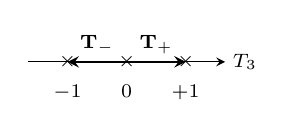
\begin{tikzpicture}[scale=0.5, >=stealth]
    % --- CONFIGURACIÓN ---
    % Eje de coordenadas (Solo existe T3)
    \draw[->, thin] (-2.5,0) -- (2.5,0) node[right] {$T_3$};

    % Coordenadas de las raíces (Valores propios del operador adjunto)
    \coordinate (O) at (0,0);
    \coordinate (Tp) at (1.5, 0);   % T+ (Sube isospín)
    \coordinate (Tm) at (-1.5, 0);  % T- (Baja isospín)

    % --- VECTORES (RAÍCES) ---
    % Mismo estilo: ultra thick
    \draw[->, thick] (O) -- (Tp) node[midway, above] {$\textbf{T}_+$};
    \draw[->,  thick] (O) -- (Tm) node[midway, above] {$\textbf{T}_-$};

    % --- CRUCES EN LOS VÉRTICES ---
    \node at (Tp) [label=below:{ $+1$}] {$\times$};
    \node at (Tm) [label=below:{ $-1$}] {$\times$};
    \node at (O)  [label=below:{ $0$}]  {$\times$}; % El centro (Cartan)

\end{tikzpicture}
\end{minipage}
- Los representantes de los generadores de SU(2) son matrices $(2j+1)\times (2j+1)$.\\
- A partir de dos multipletes $A, B$ con $j_A, j_B$ tal que $A= 2j_A+1, B=2j_B+1$,
se pueden descomponer, empleando coeficientes de C.G., en otros multipletes tal que: $$\mathbf{A} \otimes \mathbf{B} = \bigoplus_{J=|j_A - j_B|}^{j_A + j_B} \mathbf{(2J+1)} \;\;\; \rightarrow \;\;\; \prod \dim_{\otimes} = \sum \dim_{\oplus} \quad \text{e.g.}
\begin{array}{cc}
     \textbf{2} \otimes \textbf{2} = \textbf{3}\oplus \textbf{1}  \\
     \textbf{2}\otimes \textbf{3} = \textbf{4} \oplus \textbf{2}
\end{array}$$\\


\hypertarget{su3}{\section{GRUPO SU(3) - MODELO DE QUARKS}}
$\bullet$ \textbf{Generadores:} $N = 3^2 - 1 = 8$. Relación con matrices de Gell-Mann $\lambda_a$: $F_a = \frac{\lambda_a}{2}$.\\
\begin{align*}
&\lambda_1 = \left(\begin{smallmatrix}0&1&0\\1&0&0\\0&0&0\end{smallmatrix}\right)&\lambda_2 = \left(\begin{smallmatrix}0&-i&0\\i&0&0\\0&0&0\end{smallmatrix}\right)&\qquad\lambda_3 = \left(\begin{smallmatrix}1&0&0\\0&-1&0\\0&0&0\end{smallmatrix}\right)&\lambda_4 = \left(\begin{smallmatrix}0&0&1\\0&0&0\\1&0&0\end{smallmatrix}\right)\\
&\lambda_5 = \left(\begin{smallmatrix}0&0&-i\\0&0&0\\i&0&0\end{smallmatrix}\right)&\lambda_6 = \left(\begin{smallmatrix}0&0&0\\0&0&1\\0&1&0\end{smallmatrix}\right)&\qquad \lambda_7 = \left(\begin{smallmatrix}0&0&0\\0&0&-i\\0&i&0\end{smallmatrix}\right)&\lambda_8 = \frac{1}{\sqrt{3}}\left(\begin{smallmatrix}1&0&0\\0&1&0\\0&0&-2\end{smallmatrix}\right)
\end{align*}


$\bullet$ \textbf{Álgebra SU(3):} $ [F_a, F_b] = i f_{abc} F_c$ \quad $f_{abc}$: Ctes de estructura totalmente antisim.\\
$f_{123}=1$, $f_{147} = f_{246} = f_{257} = f_{345} = \frac{1}{2}$, $f_{156} = f_{367} = -\frac{1}{2}$, $f_{458} = f_{678} = \frac{\sqrt{3}}{2}$.\\
- Asimetría: $f_{abc} = -f_{bac} = -f_{cba} = -f_{acb}$\;\;\; $f_{abc} = f_{bca} = f_{cab}$ \;\;\; resto: nulos.\\

$\bullet$ \textbf{Subálgebra de Cartan (Rango 2):}
Los generadores diagonales conmutan $[F_3, F_8]=0$.
1. Isospín ($T_3$): $T_3=F_3 = \frac{1}{2}\text{diag}(1, -1, 0)$.\\
2. Hipercarga ($Y$): $Y = \frac{2}{\sqrt{3}}F_8 = \text{diag}(\frac{1}{3}, \frac{1}{3}, -\frac{2}{3})$.\\
Los autoestados se etiquetan por $(t_3, y)$ en un plano 2D.\\
$\bullet$ \textbf{Relación de Gell-Mann-Nishijima}:
$ Q = T_3 + \frac{Y}{2} \quad \text{con} \quad T_3 = I_3, \quad Y = B + S $.\\
$Q\equiv$ carga eléctrica (generador de SU(1)$_{\text{EM}}$), $B\equiv$ número bariónico, $S\equiv$ extrañeza
\begin{center}
\begin{tabular}{|c|c|c|c|c|c|c|}
\hline
\hyperlink{quarks_table}{\textbf{q}} & \textbf{$Q$} & \textbf{$T_3$} & \textbf{$Y$} & \textbf{$S$} & \textbf{$B$} & \textbf{spin}\\ \hline
$u$ & $+2/3$ & $+1/2$ & $+1/3$ & $0$ & $1/3$ & $1/2$ \\ \hline
$d$ & $-1/3$ & $-1/2$ & $+1/3$ & $0$ & $1/3$&$1/2$\\ \hline
$s$ & $-1/3$ & $0$ & $-2/3$ & $-1$ & $1/3$ & $1/2$\\ \hline
\end{tabular}\\[2pt]
Antiquarks: todos los números $Q,T_3, Y, S,B$ opuestos.
\end{center}
$\bullet$ \textbf{Operadores Escalera (Raíces):}
Se definen 3 tipos de espín en el plano $(T_3, Y)$:\\

\noindent
% BLOQUE TEXTO (55% del ancho de la columna)
\begin{minipage}[c]{0.58\linewidth}
    \raggedright % Evita espacios feos en líneas cortas
1. \textbf{I-spin ($T_\pm$):} $F_1 \pm iF_2$. $\Delta T_3 = \pm 1, \Delta Y = 0$.\\
2. \textbf{V-spin ($V_\pm$):} $F_4 \pm iF_5$. $\Delta T_3 = \mp 1/2, \Delta Y = \pm 1$.\\
3. \textbf{U-spin ($U_\pm$):} $F_6 \pm iF_7$. $\Delta T_3 = \pm 1/2, \Delta Y = \pm 1$.
\end{minipage}%
\hfill
% BLOQUE GRÁFICO (40% del ancho de la columna)
\begin{minipage}[c]{0.42\linewidth}
    \centering
    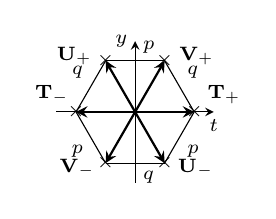
\begin{tikzpicture}[scale=0.5, >=stealth] 
    % Definición de coordenadas (vértices del hexágono)
    \coordinate (O) at (0,0);
    \coordinate (Tp) at (0:1.5);    % T+ (0 grados)
    \coordinate (Vp) at (60:1.5);   % V+ (60 grados)
    \coordinate (Up) at (120:1.5);  % U+ (120 grados)
    \coordinate (Tm) at (180:1.5);  % T- (180 grados)
    \coordinate (Vm) at (240:1.5);  % V- (240 grados)
    \coordinate (Um) at (300:1.5);  % U- (300 grados)

    % Ejes de coordenadas
    \draw[->, thin] (-2,0) -- (2,0) node[below] {$t$};
    \draw[->, thin] (0,-1.8) -- (0,1.8) node[left] {$y$};

    % Lados del hexágono y etiquetas p, q
    % La imagen muestra: 
    % Superior: p, Inferior: q
    % Diagonales superiores: q, Diagonales inferiores: p
    
    \draw (Up) -- node[above right] {$p$} (Vp);           % Superior
    \draw (Vp) -- node[above right] {$q$} (Tp);     % Superior derecha
    \draw (Tp) -- node[below right] {$p$} (Um);     % Inferior derecha
    \draw (Um) -- node[below right] {$q$} (Vm);           % Inferior
    \draw (Vm) -- node[below left] {$p$} (Tm);      % Inferior izquierda
    \draw (Tm) -- node[above left] {$q$} (Up);      % Superior izquierda

    % Vectores (Flechas gruesas desde el origen)
    \draw[->,  thick] (O) -- (Tp) node[pos=0.75, above right] {\;\; $\textbf{T}_+$};
    \draw[->,  thick] (O) -- (Vp) node[pos=0.75, above] {\qquad\quad \;\;$\textbf{V}_+$};
    \draw[->,  thick] (O) -- (Up) node[pos=0.75, above] {$\textbf{U}_{+}$ \qquad \quad \,};
    \draw[->,  thick] (O) -- (Tm) node[pos=0.75, above left] {$\textbf{T}_-$ \; };
    \draw[->,  thick] (O) -- (Vm) node[pos=0.75, below left] {$\textbf{V}_-$\;\,};
    \draw[->,  thick] (O) -- (Um) node[pos=0.75, below right] {\;\;$\textbf{U}_-$};

    % Cruces en los vértices
    \foreach \x in {Tp, Vp, Up, Tm, Vm, Um}
        \node at (\x) {$\times$};

\end{tikzpicture}

\end{minipage}


\section{REPRESENTACIONES IRREDUCIBLES SU(3)}
$\bullet$ \textbf{Diagramas de Peso:} Los estados forman hexágonos o triángulos en el plano $(T_3, Y)$.
\\$\bullet$ \textbf{Etiquetado $(p,q)$:} $p, q$ enteros $\geq 0$. Relacionados con longitud lados polígono en frontera.\\
$\bullet$ \textbf{Dimensión:} $ d(p,q) = \frac{1}{2}(p+1)(q+1)(p+q+2)$

$\bullet$ \textbf{Irreps Importantes:}\\
1. \textbf{Fundamental $\mathbf{3}$:} $(p,q)=(1,0)$.
   Quarks ($u, d, s$):  $u(\frac{1}{2}, \frac{1}{3}), d(-\frac{1}{2}, \frac{1}{3}), s(0, -\frac{2}{3})\quad (\triangle)$\\
2. \textbf{Antifundamental $\bar{\mathbf{3}}$:} $(p,q)=(0,1)$.
   Antiquarks ($\bar{u}, \bar{d}, \bar{s}$). \quad($\bigtriangledown$)\\
3. \textbf{Singlete $\mathbf{1}$:} $(p,q)=(0,0)$.\quad ($\bullet$)\\
4. \textbf{Octete $\mathbf{8}$:} $(p,q)=(1,1)$.
   \hyperlink{Mesones}{Mesones} espín 0, \hyperlink{Bariones}{Bariones} espín 1/2. \hyperlink{Gluones}{Gluones}. Rep. Adjunta.\\
5. \textbf{Decuplete $\mathbf{10}$:} $(p,q)=(3,0)$.
   \hyperlink{Bariones_big}{Bariones} espín 3/2 (Resonancias $\Delta, \Omega^-$).\\
6. \textbf{Sextete $\mathbf{6}$:} $(2,0)$ y $\bar{\mathbf{6}} (0,2)$.\\
$\bullet$ \textbf{Conjugada:} $\textbf{X}\neq\bar{\textbf{X}}$ equivalentemente $(p,q)\neq(q,p)$ (es representación c.c.). Solo: $\textbf{8}=\bar{\textbf{8}}$.\\
$\bullet$ \hyperlink{young}{\textbf{Productos Tensoriales de Irreps}} (ejemplos): $\textbf{8} \otimes {\textbf{8}} = \textbf{1} \oplus {\textbf{8}} \oplus \textbf{8} \oplus \textbf{10}\oplus \overline{\textbf{10}} \oplus {\textbf{27}}$\\
$\textbf{3} \otimes \bar{\textbf{3}} =\textbf{8}\oplus \textbf{1}$\quad$\textbf{3} \otimes {\textbf{3}} = \textbf{6} \oplus \bar{\textbf{3}}$\quad$\textbf{3} \otimes {\textbf{6}} = \textbf{8} \oplus {\textbf{10}}$\quad$\textbf{3} \otimes {\textbf{3}} \otimes \textbf{3} = \textbf{1} \oplus {\textbf{8}} \oplus \textbf{8} \oplus \textbf{10}$


\section{PROPIEDADES ALGEBRAICAS}
$\bullet$ Los productos directos cumplen propiedades distributivas, asociativas y conmutativas respecto a la suma directa.\\
$\bullet$ \textbf{Isospin Agrandado:} $SU(2) \subset SU(3)$. Las interacciones fuertes conservan $SU(3)$ (aproximadamente) y $SU(2)$ (con mayor precisión).


\section{CLASIFICACIÓN DE HADRONES -- SU(3)$_F$ (F$\equiv$ flavour)}
-- Solo podemos observar partículas libres (estados ligados) neutras de color (singletes) --
\textbf{Mesones ($q\bar{q}$)}:
Descomposición en $SU(3)_F$: $ \mathbf{3} \otimes \mathbf{\bar{3}} = \mathbf{1} \oplus \mathbf{8} $\\
\textbf{Bariones ($qqq$)}:
Descomposición en $SU(3)_F$:
$ \mathbf{3} \otimes \mathbf{3} \otimes \mathbf{3} = \mathbf{1} \oplus \mathbf{8} \oplus \mathbf{8} \oplus \mathbf{10} $\\
$\bullet$ SU(2)$_I$ (Isospín): Muy buena simetría ($m_u \approx m_d$).\\
$\bullet$ SU(3)$_F$ (Sabor): Simetría rota ($m_s > m_{u,d}$) $\Rightarrow \Delta m$ dentro de los multipletes.\\
$\bullet$ $\nexists$ SU(4) o superiores como simetrías aproximadas debido a la gran masa de $c, b, t$.



\section{FUNCIONES DE ONDA (MODELO ESTÁTICO)}
Función de onda total de un hadrón:
$\Psi_{\text{tot}} = \Psi_{\text{espacio}} \times \Psi_{\text{sabor}} \times \Psi_{\text{spin}} \times \Psi_{\text{color}} $\\
$\Psi_{\text{tot}}$ \textbf{totalmente antisimétrica} (fermiones), \textbf{totalmente simétrica} (bosones).

\textbf{Construcción del Protón ($p^\uparrow$)}:\\
-- Paridad $\Psi_{\text{espacio}}$: $(-1)^L$. Estado fundamental ($L=0$) $\implies$ 
simétrica.\\
Combinación Flavor-Spin debe ser simétrica (para compensar antisimetría de color).\\
Base de Flavour ($uud$):\\
$\bullet$ Simétrica ($1\leftrightarrow 2$): $\phi_S = \frac{1}{\sqrt{6}}[(ud+du)u - 2uud]$.\\
$\bullet$ Antisimétrica ($1\leftrightarrow 2$): $\phi_A = \frac{1}{\sqrt{2}}(ud-du)u$.\\
Base de Spin ($\uparrow\uparrow\downarrow$):\\
$\bullet$ Simétrica ($1\leftrightarrow 2$): $\chi_S = \frac{1}{\sqrt{6}} [\uparrow\downarrow\uparrow + \downarrow\uparrow\uparrow -2 \uparrow\uparrow\downarrow]$ (Espín 1).\\
$\bullet$ Antisimét ($1\leftrightarrow 2$): $\chi_A = \frac{1}{\sqrt{2}} [\uparrow\downarrow\uparrow-\downarrow\uparrow\uparrow]$ (Espín 0).\\
-- \text{Función Flavour-Spin}: $ \Psi_{F-S}(p^\uparrow) = \frac{1}{\sqrt{2}} (\phi_S \chi_S + \phi_A \chi_A) $ = 
$$= | p \uparrow\rangle   = \frac{1}{\sqrt{18}} [2|u\!\uparrow u\!\uparrow d\!\downarrow\rangle - |u\!\uparrow u\!\downarrow \!d\uparrow\rangle - |u\!\downarrow u\!\uparrow d\!\uparrow\rangle + \text{perms} ] $$
perms: permutaciones \underline{cíclicas} de los pares (quarks-espín)

\section{MOMENTOS MAGNÉTICOS}
Operador: $\vec{\mu} = \sum_i \mu_i \vec{\sigma}_i$.
Donde $\mu_q = Q_q (\frac{e}{2m_q})$.
Valor esperado $\langle p\uparrow | \mu_z | p\uparrow \rangle$:
$$ \mu_p = \frac{1}{3}(4\mu_u - \mu_d) \qquad  \mu_n = \frac{1}{3}(4\mu_d - \mu_u) $$




\section{COLOR SU(3)$_c$}
\textbf{Carga de Color}: $R= \textbf{q}_1,\,G=\textbf{q}_2, \, B = \textbf{q}_3$ (Fundamental $\mathbf{3}$ de $SU(3)_c$).\\
\textbf{Confinamiento}:
Los hadrones observados son \textbf{Singletes de Color} ($\mathbf{1}$).\\
$\Psi_{\text{color}}$ debe ser totalmente antisimétrica e invariante bajo rotaciones en el espacio de color.


\textbf{Singlete Bariónico ($qqq$)}:
$ \mathbf{1} \in \mathbf{3} \otimes \mathbf{3} \otimes \mathbf{3} $
$$ \Psi_{\text{color}} = \frac{1}{\sqrt{6}} \epsilon_{ijk} |q_i q_j q_k\rangle = \frac{1}{\sqrt{6}}(RGB - RBG + BRG - BGR + GBR - GRB) $$

\textbf{Singlete Mesónico ($q\bar{q}$)}:
$ \mathbf{1} \in \mathbf{3} \otimes \mathbf{\bar{3}} $
$$ \Psi_{\text{color}} \!=\! \frac{1}{\sqrt{3}} (R\bar{R} + G\bar{G} + B\bar{B}) \quad \bar{R}= \frac{1}{\sqrt{2}} (GB-BG)\quad \bar{G} =  \frac{1}{\sqrt{2}} (BR-RB)\quad  \bar{B} = \frac{1}{\sqrt{2}} (RG-GR)$$


\section{MODELO DE PARTONES (FEYNMAN 1969)}
\textbf{Composición Hadrones:}\\
$\bullet$ \textbf{Quarks de valencia ($q_v$):} Definen n$^\text{os}$ cuánticos. e.g.: $p$ ($u_v u_v d_v$), $n$ ($d_v d_v u_v$).\\
$\bullet$ \textbf{Partones del mar (Sea Partons):} Pares $q\bar{q}$ (prob< no nula de excitación) y gluones ($g$). Participan en reparto energético, no en números cuánticos globales. \\

\textbf{Cinemática (Infinite Momentum Frame):}\\
$\bullet$ Protón con momento $P$ y energía $E$. Partón $i$ lleva fracción $x$ del momento. \\
$\bullet$ \textbf{Variable de Bjorken:} $x = p_{\text{parton}}/P_{\text{proton}}$, con $0 \le x \le 1$. \\
$\bullet$ Momentos: $p_i^\mu \approx x P^\mu$. Transverso ($\perp$) $P_T \approx 0$, Longitudinal ($\parallel$) $P_L \neq0$ (respecto haz). \\
$\bullet$ Masa hadrón y partones se desprecian a altas energías ($s \gg M^2$).

\section{FUNCIONES DE DISTRIBUCIÓN DE PARTONES (PDFs)}
\textbf{PDF ($f_i(x)$):}
Probabilidad de hallar partón tipo $i$ con fracción de momento $x$ en el hadrón.\\
$\bullet$ \textbf{Regla de suma (Momentum Sum Rule):} Conservación del momento total del protón.
$$ \sum_{i} \int_0^1 x f_i(x) dx = 1 $$
La suma $i$ incluye valencia, sea y gluones. Experimentos: gluones $\sim 50\%$ del momento.

\textbf{Tipos y Nomenclatura:}\\
$\bullet$ Valencia: $u_v, d_v$. Sea: $u_s, d_s, s_s, \dots$ y antiquarks $\bar{u}, \bar{d}, \bar{s}$. \\
$\bullet$ Simetría del mar: $q_s(x) = \bar{q}_s(x)$. \\
$\bullet$ PDFs totales: $u(x) = u_v(x) + u_s(x)$, $\bar{u}(x) = \bar{u}_s(x)$. \\
$\bullet$ Protón tiene $2u$ y $1d$: $\int_0^1 (u(x)-\bar{u}(x))dx = 2$, $\int_0^1 (d(x)-\bar{d}(x))dx = 1$.

\textbf{Comportamiento ``Naive":}\\
$\bullet$ \textbf{Valencia:} Domina en $x \sim 1/3$. \\
$\bullet$ \textbf{Sea/Gluones:} Dominan a bajo $x$ ($x \to 0$). Divergencia infrarroja regularizada.

\section{TEOREMA DE FACTORIZACIÓN}
Separación del proceso hadrónico en:\\
1. \textbf{Soft Physics:} PDFs (No perturbativo, universal).\\
2. \textbf{Hard Physics:} Sección eficaz partónica $\hat{\sigma}$ (Perturbativo, calculable).

\textbf{Fórmula General (Colisión $P_1 + P_2$):}
$$ \sigma_{\text{tot}}(s) = \sum_{i,j} \int_0^1 dx_1 \int_0^1 dx_2 f_i(x_1) f_j(x_2) \hat{\sigma}_{ij}(\hat{s}) $$
$\bullet$ $x_{1,2}$: Fracción momento partones 1 y 2. \\
$\bullet$ $s = (P_1+P_2)^2 \approx 2P_1 P_2$. \\
$\bullet$ $\hat{s} = (x_1 P_1 + x_2 P_2)^2 \approx x_1 x_2 s$. \\
$\bullet$ $\hat{\sigma}_{ij}$: Sección eficaz subproceso elemental $i+j \to \text{final}$.



\section{PROCESOS DE COLISIÓN ESPECÍFICOS}
\textbf{1. Electrón-Protón ($ep \to e^- X$, DIS):}
Sonda: Fotón virtual $\gamma^*$ (o $Z$) con $Q^2 = -q^2$.
$$ \sigma(ep \to eX) = \sum_i \int_0^1 dx f_i(x) \hat{\sigma}(eq_i \to eq_i) $$
$\bullet$ Diagrama: Scattering $e^-$ sobre quark libre $q_i$. \\
$\bullet$ Estado final: $e^-$ saliente + Jet hadrónico (quark) + Remanente protón (dirección haz).

\textbf{2. Protón-Antiprotón ($p\bar{p} \to \ell^+\ell^- X$, Drell-Yan):}
Aniquilación $q_i \bar{q}_i \to \gamma^*/Z \to \ell^+ \ell^-$.
$$ \sigma = \sum_{i} \int dx_1 dx_2 [f_i(x_1) f_{\bar{i}}(x_2) + f_{\bar{i}}(x_1) f_i(x_2)] \hat{\sigma}(q\bar{q} \to \ell\ell) $$
$\bullet$ Requiere un quark de valencia y un antiquark (valencia en $\bar{p}$ o sea en $p$).

\textbf{3. Protón-Protón ($pp \to W^\pm X$):}
Producción bosón $W$ vía interacción débil.
$$ \sigma = \sum_{i,j} \int dx_1 dx_2 f_i(x_1) f_j(x_2) V_{CKM}^2 \hat{\sigma}(q_i \bar{q}_j \to W) $$
$\bullet$ Ejemplo $u \bar{d} \to W^+$. Antiquark debe provenir del mar (sea) en colisiones $pp$.

\section{FUNCIONES DE ESTRUCTURA Y $Q^2$}
\textbf{Función $F_2(x, Q^2)$:}
Relaciona sección eficaz medida con contenido partónico.
$$ F_2(x, Q^2) = \sum_i e_i^2 x f_i(x, Q^2) $$
$\bullet$ $e_i$: Carga eléctrica quark ($u=2/3, d=-1/3$). \\
    $\bullet$ Gluones no contribuyen directamente a $F_2$ en orden más bajo (LO), solo q/$\bar{\text{q}}$ cargados.

\textbf{Scaling de Bjorken:}\\
$\bullet$ Predicción Partones (Naive): $F_2(x, Q^2) \to F_2(x)$. Indep de $Q^2$ si partones puntuales.\\
$\bullet$ \textbf{Violación del Scaling:} Experimentalmente $F_2$ depende de $Q^2$.\\
- $x$ bajos: $F_2$ crece con $Q^2$ (aumenta densidad partones sea/gluones al aumentar resolución).\\
- $x$ altos: $F_2$ decrece con $Q^2$ (quarks valencia radian gluones y pierden momento).

\section{EVOLUCIÓN QCD (DGLAP)}
El modelo de partones estático no predice dependencia en $Q^2$. QCD introduce evolución vía emisión de gluones (splitting).\\
$\bullet$ Escala $Q^2$: Resolución espacial probe $\sim 1/\sqrt{Q^2}$.\\
$\bullet$ \textbf{Ecuaciones DGLAP:} Describen variación de PDFs con $\ln Q^2$.\\

\textbf{Ejemplo (Evolución del Gluón):}
$$ \frac{d g(x,Q^2)}{d \ln Q^2} = \frac{\alpha_s(Q^2)}{2\pi} \int_x^1 \frac{dy}{y} \left[ \sum_q P_{gq}\left(\frac{x}{y}\right) q(y,Q^2) + P_{gg}\left(\frac{x}{y}\right) g(y,Q^2) \right] $$
$\bullet$ $\alpha_s$: Constante acoplamiento fuerte. \\
$\bullet$ $P_{ba}(z)$: Funciones de splitting. Probabilidad proceso $a \to b$ con fracción $z$.\\
- $P_{qq}$: Quark radia gluón (queda quark).\\
- $P_{gq}$: Quark radia gluón (queda gluón).\\
- $P_{gg}$: Gluón se divide en gluones ($g \to gg$).\\
- $P_{qg}$: Gluón crea par $q\bar{q}$.\\




% \hrule

\section{DIAGRAMAS DE FEYNMAN (FD): GENERALIDADES}
Representación gráfica en el \textbf{espacio de momentos}. \\
$\bullet$ \text{Ejes:} Eje temporal de izquierda (IN) a derecha (OUT).\\
$\bullet$ Conservación $P^\mu$ en cada vértice y globalmente.\\
$\bullet$ Líneas Internas: Virtuales (off-shell: $p^2 \neq m^2$).\\
$\bullet$ Líneas externas (patas): Reales (on-shell: $p_i^2 = m_i ^2$).\\
$\bullet$ Amplitud Invariante $(F \text{ o } \mathcal{M})$:
$$T_{fi} = - i (2\pi)^4 \delta^{(4)}(P_{\text{tot}}) F \qquad P_{\text{tot}}= P_{\text{in}} - P_{\text{out}}$$
$$ -iF = (\text{Vértices}) \times (\text{Propagadores}) \times (\text{Patas Ext.}) $$


\section{GUÍA DE TRAZADO LÍNEAS}
\begin{center}
\begin{tabular}{cll}
\textbf{Trazo} & \textbf{Estilo Visual} & \textbf{Partícula} \\
\hline
\tikz[baseline=-3pt]{\draw[fermion] (0,0) -- (1,0);} & Línea cont. + Flecha & \textbf{Fermión} ($e^-, \mu, q,  \nu$) \\
\tikz[baseline=-3pt]{\draw[antifermion] (0,0) -- (1,0);} & Flecha opuesta & \textbf{Antifermión} ($e^+, \bar{q}$) \\
\tikz[baseline=-3pt]{\draw[photon] (0,0) -- (1,0);} & Ondulada (Snake) & \textbf{Fotón} ($\gamma, W, Z$) \\
\tikz[baseline=-3pt]{\draw[scalar] (0,0) -- (1,0);} & Discontinua (Dashed) & \textbf{Escalar} ($\pi, K,$\textit{Higgs}) \\
\tikz[baseline=-3pt]{\draw[gluon] (0,0) -- (1,0);} & Bucle (Coil) & \textbf{Gluón} ($g$) \\
\end{tabular}\\
$\bullet$ \textbf{Flechas}: Indican flujo de carga fermiónica (NO siempre coinciden con el momento).
\end{center}
\section{CANALES DE MANDELSTAM ($1+2 \to 3+4$)}
Amplitud total $F = F_s + F_t + F_u$. \quad\quad $s+t+u = m_A^2+ m_B^2 + m_C^2 + m_D^2$
\begin{center}
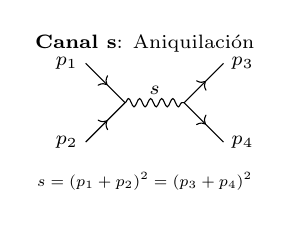
\begin{tikzpicture}[scale=0.5, baseline=(current bounding box.center)]
\node at (1.5,2.5) {\textbf{Canal s}: Aniquilación};
\draw[fermion] (0,2) node[left]{$p_1$} -- (1,1);
\draw[fermion] (0,0) node[left]{$p_2$} -- (1,1);
\draw[photon] (1,1) -- (2.5,1) node[midway, above]{$s$};
\draw[fermion] (2.5,1) -- (3.5,2) node[right]{$p_3$};
\draw[fermion] (2.5,1) -- (3.5,0) node[right]{$p_4$};
\node at (1.5, -1) {\scalebox{0.8}{$s = (p_1+p_2)^2 =(p_3+p_4)^2$}};
\end{tikzpicture}
\hspace{5pt}
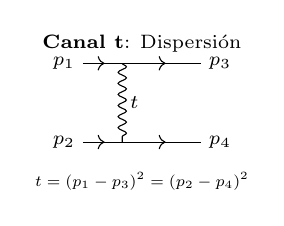
\begin{tikzpicture}[scale=0.5, baseline=(current bounding box.center)]
\node at (1.5,2.5) {\textbf{Canal t}: Dispersión};
\draw[fermion] (0,2) node[left]{$p_1$} -- (1,2);
\draw[fermion] (1,2) -- (3,2) node[right]{$p_3$};
\draw[photon] (1,2) -- (1,0) node[midway, right]{$t$};
\draw[fermion] (0,0) node[left]{$p_2$} -- (1,0);
\draw[fermion] (1,0) -- (3,0) node[right]{$p_4$};
\node at (1.5, -1) {\scalebox{0.8}{$t = (p_1-p_3)^2=(p_2-p_4)^2$}};
\end{tikzpicture}
\hspace{5pt}
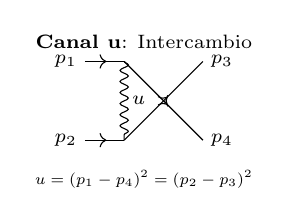
\begin{tikzpicture}[scale=0.5, baseline=(current bounding box.center)]
\node at (1.5,2.5) {\textbf{Canal u}: Intercambio};
\draw[fermion] (0,2) node[left]{$p_1$} -- (1,2);
\draw[fermion] (1,0) -- (3,2) node[right]{$p_3$};
\draw[photon] (1,2) -- (1,0) node[midway, right]{$u$};
\draw[fermion] (0,0) node[left]{$p_2$} -- (1,0);
\draw[fermion] (1,2) -- (3,0) node[right]{$p_4$};
\node at (1.5, -1) {\scalebox{0.8}{$u = (p_1-p_4)^2=(p_2-p_3)^2$}};
\end{tikzpicture}
\end{center}
CM, $m \to 0$:\;\; $s = 4E^2 $\qquad\;\;\qquad\qquad$t= -\frac{s}{2}(1 - \cos\theta)$\qquad\qquad $u= -\frac{s}{2}(1 + \cos\theta)$ 

\section{REGLAS: PROPAGADORES (Internos)}
Inverso de la función de Green de 2 puntos en el espacio de momentos.\\
$\mathcal{FT}$ al espacio de momentos: $i\partial^\mu \rightarrow p^\mu \quad  \square^2 = \partial_\mu \partial^\mu \rightarrow -p^2\quad \frac{1}{\square^2 + m^2} \rightarrow\frac{1}{-p^2 + m^2} $\\
\textbf{1. Escalar} (spin 0, $m$): $\Delta(p) = \frac{i}{p^2 - m^2}$\\
\textbf{2. Fermión} (spin $1/2$, $m$): $S_F(p) = \frac{i(\cancel{p} + m)}{p^2 - m^2}$\\
\textbf{3. Fotón} (spin 1, $m=0$, Feynman): $D_{\mu\nu}(p) = \frac{-i g_{\mu\nu}}{p^2} = \frac{-i g_{\nu \mu}}{k^2}$

\section{REGLAS: VÉRTICES DE INTERACCIÓN -- $V^\mu = FR \equiv$ Feymann Rule}
Multiplica $i$ por $\mathcal{L}_{\text{int}}$ (solamente la parte relevante de $\mathcal{L}_{\text{int}}$ en el espacio de momentos: no normalización y no campos externos: e.g. $A_\mu$, $e^{i(p_{\text{f}}- p_{\text{i}})x}, \dots$).\\

\begin{minipage}{0.49\linewidth}
\textbf{1. Escalar:} Bosón cargado $\phi$ - Fotón $A_\mu$ 
\begin{center}
$\mathcal{L}_{\text{int}} \propto J^\mu A_\mu$\vspace{3pt}
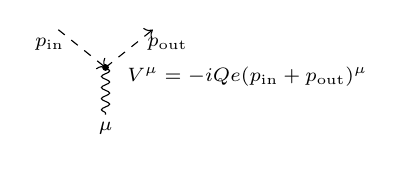
\begin{tikzpicture}[scale=0.6, baseline=(current bounding box.center)]
\draw[scalar, ->] (-1,0.8) -- (0,0) node[near end, above left]{$p_{\text{in}}\quad$};
\draw[scalar, ->] (0,0) -- (1,0.8) node[near start, above right]{$\quad p_{\text{out}}$};
\draw[photon] (0,0) -- (0,-1) node[below]{$\mu$};
\node[vertex] at (0,0) {};
\node at (3,-0.2) {$V^\mu = -i Q e (p_{\text{in}} + p_{\text{out}})^\mu$};
\end{tikzpicture}
\end{center}
\end{minipage}
\begin{minipage}{0.49 \linewidth}
\textbf{2. Fermiónica:} Fermión $\psi$ - Fotón $A_\mu$ 
\begin{center}
$\mathcal{L}_{\text{int}} = -e Q \bar{\psi} \gamma^\mu \psi A_\mu$\vspace{3pt}
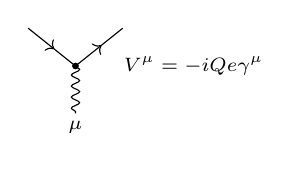
\begin{tikzpicture}[scale=0.6, baseline=(current bounding box.center)]
\draw[fermion] (-1,0.8) -- (0,0);
\draw[fermion] (0,0) -- (1,0.8);
\draw[photon] (0,0) -- (0,-1) node[below]{$\mu$};
\node[vertex] at (0,0) {};
\node at (2.5,0) {$V^\mu = -i Q e \gamma^\mu$};
\end{tikzpicture}
\end{center}    
\end{minipage}



\section{TEOREMAS DE TRAZAS (TRUCO DE CASIMIR)}
$\Gamma$ cualquier producto de matrices de Dirac. $\bar{\Gamma} = \gamma^0 \Gamma^\dagger\gamma^0$\\
$\bullet$ \textbf{Relación}: $[\bar{u}(p',s')\, \Gamma\, u(p,s)]^\dagger = \bar{u}(p,s)\, \bar{\Gamma}\, u(p',s').$ 
\\ $\bullet$ If $\Gamma=\gamma^\mu:$ $[\bar{u}(p',s')\, \gamma^\mu\, u(p,s)]^\dagger = \bar{u}(p,s)\, \gamma^\mu\, u(p',s').$\\
$\bullet$ \textbf{Tip}: $\sum_{s_1, s_3}| \bar{u}_3 \gamma^\mu u_1 |^2 = \sum_{s_1, s_3}(\bar{u}_3 \gamma^\mu u_1)(\bar{u}_1 \gamma^\nu u_3)= \text{Tr}[(\cancel{p}_3 + m_3)\gamma^\mu (\cancel{p}_1 + m_1)\gamma^\nu]$.





\section{CÁLCULO DE SECCIÓN EFICAZ ($\sigma$)}
Relación entre Amplitud Invariante $F$ (o $\mathcal{M}$) y observables.\\
$\bullet$ \textbf{Sección Eficaz Diferencial} ($A+B \to C+D$ en CM):
$$ d\sigma = \frac{1}{2E_{CM} |\vec{v}_A - \vec{v}_B|} |\bar{F}|^2 d\Phi_2= \frac{1}{2\lambda^{1/2} (s, m_A^2, m_B^2)} |\vec{F}|^2 \, dLips(s, p_C, p_D) $$
$$\lambda^{1/2} (s, m_A^2, m_B^2) = 2 \sqrt{(p_A \cdot p_B)^2 - m_A^2 m_B^2}$$
$$ d{Lips}(s, p_C, p_D)  = (2\pi)^4 \delta^4(p_A+p_B- p_C -p_D) \frac{d^3\vec{p}_C}{(2\pi)^3 2E_C} \frac{d^3\vec{p}_D}{(2\pi)^3 2E_D}$$

$$\delta^4 (p_1 +p_2-p_3 -p_4) = \delta (E_1+E_2-E_3-E_4) \delta^3(\vec{p_1}+\vec{p_2}-\vec{p_3}-\vec{p_3})$$

$$ \textbf{Promedio de spin} \text{ (si no son escalares):}\quad|\bar{F}|^2 = \frac{1}{(2S_A+1)(2S_B+1)} \sum_{\text{spins}} |F|^2 $$
$$\text{Si la partícula $i$ es un \textbf{fotón}, no se emplea $(2S_i +1),$ sino que se divide entre 2}$$
$$ \frac{d\sigma}{d\Omega_{CM}} = \frac{1}{64\pi^2 s} \frac{|\vec{p}_f|}{|\vec{p}_i|} |\bar{F}|^2 \qquad \frac{d\sigma}{dt}= \frac{1}{16\pi} \frac{1}{\lambda(s, m_1^2, m_2^2)} |\bar{F}|^2 $$





% \section{EJEMPLO DISPERSIÓN $e^- \mu^- \to e^- \mu^-$ (QED)}
% \textbf{Diagrama (Canal t)}: Único diagrama (partículas distinguibles).
% \begin{center}
% \begin{tikzpicture}[scale=0.6]
% \draw[fermion] (-1,1) node[left]{$e^-(p_1)$} -- (0,0.5);
% \draw[fermion] (0,0.5) -- (1,1) node[right]{$e^-(p_3)$};
% \draw[photon] (0,0.5) -- (0,-0.5) node[midway, right]{$q$};
% \draw[fermion] (-1,-1) node[left]{$\mu^-(p_2)$} -- (0,-0.5);
% \draw[fermion] (0,-0.5) -- (1,-1) node[right]{$\mu^-(p_4)$};
% \node at (0.0, 0.9) {$\mu$};
% \node at (0.0, -0.9) {$\nu$};
% \end{tikzpicture}
% \end{center}
% $$ -iF = \underbrace{\{\bar{u}(p_3) (+ie\gamma^\mu) u(p_1)\}}_{\text{Corriente } e^-} \underbrace{\left(\frac{-ig_{\mu\nu}}{q^2}\right)}_{\text{Prop. Fotón}} \underbrace{\{\bar{u}(p_4) (+ie\gamma^\nu) u(p_2)\}}_{\text{Corriente } \mu^-} $$
% $$ F = -\frac{e^2}{t} [\bar{u}_3 \gamma^\mu u_1] [\bar{u}_4 \gamma_\mu u_2] $$
% $$ |\bar{F}|^2 = \frac{e^4}{4t^2} \text{Tr}[(\cancel{p}_3+m_e)\gamma^\mu(\cancel{p}_1+m_e)\gamma^\nu] \text{Tr}[(\cancel{p}_4+m_\mu)\gamma_\mu(\cancel{p}_2+m_\mu)\gamma_\nu] $$
% \textbf{Resultado (Límite Ultrarelativista $m \to 0$)}:
% Usando Mandelstam ($s, t, u$):
% $$ |\bar{F}|^2 \approx \frac{2e^4}{t^2} (s^2 + u^2) \qquad \frac{d\sigma}{d\Omega} = \frac{\alpha^2}{2s} \frac{s^2+u^2}{t^2} $$

\section{PROCESOS QED (DIAGRAMAS)}

\textbf{1. Aniquilación $e^- e^+ \to \mu^- \mu^+$}:
Solo canal s (carga total 0, muones distinguibles).
\begin{center}
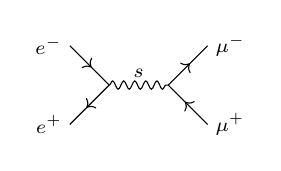
\begin{tikzpicture}[scale=0.5]
\draw[fermion] (-1,1) node[left]{$e^-$} -- (0,0);
\draw[antifermion] (-1,-1) node[left]{$e^+$} -- (0,0);
\draw[photon] (0,0) -- (1.5,0) node[midway, above]{$s$};
\draw[fermion] (1.5,0) -- (2.5,1) node[right]{$\mu^-$};
\draw[antifermion] (1.5,0) -- (2.5,-1) node[right]{$\mu^+$};
\end{tikzpicture}
\end{center}

\textbf{2. Dispersión Møller $e^- e^- \to e^- e^-$}:
Partículas iguales. Interferencia Canal t + Canal u.
\begin{center}
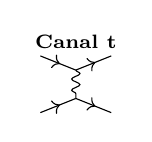
\begin{tikzpicture}[scale=0.45]
\node at (0,1.2) {\textbf{Canal t}};
\draw[fermion] (-1,0.8) -- (0,0.4); \draw[fermion] (0,0.4) -- (1,0.8);
\draw[photon] (0,0.4) -- (0,-0.4);
\draw[fermion] (-1,-0.8) -- (0,-0.4); \draw[fermion] (0,-0.4) -- (1,-0.8);
\end{tikzpicture}
\hspace{0.2cm}

\begin{tikzpicture}[scale=0.45]
\node at (0,1.2) {\textbf{Canal u}};
\draw[fermion] (-1,0.8) -- (0,0.4); 
\draw[fermion] (0,-0.4) -- (1,0.8); % Cruzado
\draw[photon] (0,0.4) -- (0,-0.4);
\draw[fermion] (-1,-0.8) -- (0,-0.4); 
\draw[fermion] (0,0.4) -- (1,-0.8); % Cruzado
\end{tikzpicture}
\end{center}
$$ F = F_t - F_u \quad (\text{Signo relativo - por Fermi}) $$

\textbf{3. Dispersión Bhabha $e^- e^+ \to e^- e^+$}:
Canal s (aniquilación) + Canal t (scattering).
\begin{center}
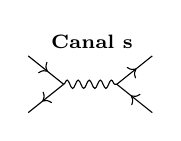
\begin{tikzpicture}[scale=0.45]
\node at (0.8,1.2) {\textbf{Canal s}};
\draw[fermion] (-1,0.8) -- (0,0);
\draw[antifermion] (-1,-0.8) -- (0,0);
\draw[photon] (0,0) -- (1.5,0);
\draw[fermion] (1.5,0) -- (2.5,0.8);
\draw[antifermion] (1.5,0) -- (2.5,-0.8);
\end{tikzpicture}
\hspace{0.2cm}
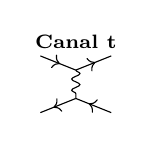
\begin{tikzpicture}[scale=0.45]
\node at (0,1.2) {\textbf{Canal t}};
\draw[fermion] (-1,0.8) -- (0,0.4); \draw[fermion] (0,0.4) -- (1,0.8);
\draw[photon] (0,0.4) -- (0,-0.4);
\draw[antifermion] (-1,-0.8) -- (0,-0.4); \draw[antifermion] (0,-0.4) -- (1,-0.8);
\end{tikzpicture}
\end{center}

\textbf{4. Compton $e^- \gamma \to e^- \gamma$}:
Canal s + Canal u (Diagramas con propagador fermiónico).




\section{LAGRANGIANO DE QED}
Construcción mínima invariante $U(1)_{\text{EM}}$ y Lorentz:
$$\mathcal{L}_{QED} = \mathcal{L}_{\text{Dirac}} + \mathcal{L}_{\text{Maxwell}} + \mathcal{L}_{\text{int}}$$
$$\mathcal{L}_{\text{Dirac}}=  \bar{\psi} (i \cancel{\partial} - m) \psi \qquad \mathcal{L}_{\text{Maxwell}} = -\frac{1}{4} F_{\mu \nu }F^{\mu \nu} \qquad \mathcal{L}_{\text{int}} =-J_\mu^\psi A^\mu \;\;\; J_\mu^\psi = eQ\bar{\psi}\gamma^\mu\psi$$
$$\mathcal{L}_{QED} = \bar{\psi}(i\cancel{D} - m)\psi - \frac{1}{4}F_{\mu\nu}F^{\mu\nu}$$
$\bullet$ \textbf{Ecuaciones de Movimiento}:
Dirac: $(i\cancel{D} - m)\psi = 0$.
Maxwell: $\partial_\nu F^{\nu\mu} = J^\mu$.


\section{INVARIANCIA GAUGE U(1)}
\textbf{Global}: $\psi \to e^{-iQ\theta}\psi$ \;\; $\bar{\psi} \to \bar{\psi}e^{+iQ\theta}$\;\;$\partial_\mu\psi \to e^{-iQ\theta}\partial_\mu\psi$ ($\theta = \text{cte}$). $\mathcal{L}_{\text{Dirac}}$ es invariante.\\
\textbf{Local}: $\psi \to e^{-iQ\theta(x)}\psi$. Requiere introducir campo gauge $A_\mu$.\\
$\bullet$ \textbf{Derivada Covariante}: $ D_\mu = \partial_\mu + ieQA_\mu$
\\Transformación del campo gauge para mantener invarianza:
$A_\mu \to A_\mu + \frac{1}{e}\partial_\mu \theta(x)$\\

$\bullet$ \textbf{Tensor de Campo}: $F_{\mu\nu} = \partial_\mu A_\nu - \partial_\nu A_\mu$. Es invariante gauge ($F'_{\mu\nu} = F_{\mu\nu}$).




\section{VECTORES DE POLARIZACIÓN $\varepsilon^\mu (q)$ \qquad $k = q \equiv$ momento del fotón}

\textbf{Condición Lorentz}: $\partial_\mu A^\mu \!= \!0 \!\Rightarrow \!A^\mu = \varepsilon^\mu (q) \, e^{-iq\cdot x}$\quad$q_\mu \varepsilon^\mu(q)\!=\!0\quad k^2\!=\! 0\Leftrightarrow$ fotón real


$\bullet$ \textbf{Suma de Polarizaciones} (Completitud): $ \sum_{\lambda=1,2} \varepsilon_\mu^{(\lambda)} (q) \varepsilon_\nu^{(\lambda)*}(q) = -g_{\mu\nu} $\\

$\bullet$ dof = 2. \quad Dado $q^\mu = (E, 0,0,|q|) \Rightarrow E = |q|$ y las polarizaciones son: \\$$\varepsilon^{(\lambda=+1)}_\mu(q) = \frac{1}{\sqrt{2}}(0,1,+i,0) \qquad \varepsilon_\mu^{(\lambda=-1)}(q) = -\frac{1}{\sqrt{2}}(0,1,-i,0)$$

Vector de polarización $\epsilon^\mu$: Codifica la orientación espacial del espín de la partícula, describiendo físicamente cómo se proyecta su momento angular intrínseco (helicidad) a lo largo de su trayectoria.

\section{FIJACIÓN DE GAUGE ($R_\xi$)}
Se debe introducir  $ \mathcal{L}_{GF} = -\frac{1}{2\xi}(\partial_\mu A^\mu)^2,\;\ \xi \in \mathbb{R}$
en $\mathcal{L}_{QED}$ para fijar el Gauge.\\

$\bullet$ Modifica las ecuaciones de movimiento pero hace el propagador invertible.\\ 
$\bullet$ \textbf{Observables}: Independientes del parámetro $\xi$.

$\bullet$ \textbf{Propagador del Fotón}: Obtenido invirtiendo el operador cinético cuadrático.
$$i\Delta_{\mu\nu}(k) = \frac{-i}{k^2 + i\epsilon} \left[ g_{\mu\nu} + (\xi - 1)\frac{k_\mu k_\nu}{k^2} \right]$$

$\cdot$ \textbf{Feynman-'t Hooft} ($\xi = 1$):
   $\Delta_{\mu\nu} \propto \frac{g_{\mu\nu}}{k^2} $ \quad $\cdot$ \textbf{Landau} ($\xi = 0$):
   $\Delta_{\mu\nu} \propto \frac{g_{\mu\nu} - k_\mu k_\nu/k^2}{k^2}$



\section{ANÁLISIS DIAGRAMAS DE FEYNMAN}
\textbf{1. Asignar momentos:} A cada partícula se le asigna un momento $p_i$.\\
\textbf{2. Dibujar diagramas:} Se dibujan todos los posibles diagramas (canal $s$, $t$ y $u$). \\
Descarta aquellos diagramas que no conserven las cantidades de la tabla:

{
\centering
\begin{center}
\begin{tabular}{|l|c|c|c|}
\hline
\textbf{Cantidad} & \textbf{Fuerte} & \textbf{Electromagnética} & \textbf{Débil} \\ \hline
Energía/Momento ($p^\mu$) & Sí & Sí & Sí \\ \hline
Momento angular total & Sí & Sí & Sí \\ \hline

Carga Eléctrica ($Q$) & Sí & Sí & Sí \\ \hline
Carga de Color & Sí & --- & --- \\ \hline
Sabor (Quarks) & Sí & Sí & No (vía $W^\pm$) \\ \hline
Paridad ($P$) & Sí & Sí & No \\ \hline
Conjugación de Carga ($C$) & Sí & Sí & No \\ \hline
G-Paridad ($G$) & Sí & No & No \\ \hline
Simetría $CP$ & Sí & Sí & No (violación) \\ \hline
Isospin ($I$) & Sí & No & No \\ \hline
3ª Componente Isospin ($I_3$) & Sí & Sí & No \\ \hline
\end{tabular}
\end{center}

}


\textbf{3. Aplicar Feynman Rules:} Se leen los diagramas de Feynmann aplicando FR. Tips:\\
$\vdash$ Vértices distintos tienen índices distintos.\\
$\vdash$ Partícula \textit{ingoing} con momento $p$ $\;\; \equiv \;\; $ Antipartícula \textit{outgoing} con momento $-p$.\\
$\vdash$ Si dos diagramas son idénticos salvo por el intercambio de dos \underline{fermiones} externos, se multiplica por $(-1)$ una de las dos amplitudes invariantes.\\
$\vdash$ Las líneas \underline{fermiónicas} se leen al revés.

\textbf{4. Cálculo $|F|^2$ y $|\bar{F}|^2$:} Se calcula $|F|^2 = F\cdot F^*$. Nota: $F$ y $F^*$ con distintos 
índices.\\

\textbf{5.} Producto espacio espinorial, relaciones de completitud y expresarlo en términos de trazas.\\

\textbf{6. Cálculo de trazas:} Se calculan trazas, y se contraen con $\eta_{\mu_\mu} \eta ^{\rho \sigma}$.\\

$\bullet$ Crossing: $s\leftrightarrow t \;\;\Leftrightarrow \;\;p_3 \leftrightarrow -p_2 \; \& \; m_3 \leftrightarrow m_2$ (evitas recalcular $|\bar{F}|^2$ si consigues $\textit{isomorfear}$ a un diagrama equivalente). Ídem para $s\leftrightarrow u$ y $t \leftrightarrow u$.


\textbf{7.} Cálculo de la sección eficaz.





\section{PROCESO DE ANIQUILACIÓN ($e^- e^+ \to \mu^- \mu^+$)}

\textbf{Amplitud ($F_s$):}
Lectura del diagrama (recordar sentido opuesto a flechas fermiónicas):
$$ -iF = [\bar{u}(p_3) (ie\gamma^\mu) v(p_4)] \frac{-ig_{\mu\nu}}{s} [\bar{v}(p_2) (ie\gamma^\nu) u(p_1)] $$
Simplificación ($m_e \approx 0$ frente a $m_\mu$ o energías altas):
$$ F = \frac{e^2}{s} [\bar{u}_3 \gamma^\mu v_4] [\bar{v}_2 \gamma_\mu u_1] $$

\textbf{Cuadrado de Amplitud Promediada:}
$$ |\overline{F}|^2 = \frac{e^4}{4s^2} \text{Tr}[(\cancel{p}_3+m_\mu)\gamma^\mu(\cancel{p}_4-m_\mu)\gamma^\nu] \text{Tr}[(\cancel{p}_2-m_e)\gamma_\mu(\cancel{p}_1+m_e)\gamma_\nu] $$
Resultado exacto (con masas):
$$ |\overline{F}|^2 = \frac{2e^4}{s^2} \{ (p_1 \cdot p_3)(p_2 \cdot p_4) + (p_1 \cdot p_4)(p_2 \cdot p_3) + m_\mu^2(p_1 \cdot p_2) \} $$
Límite Ultra-Relativista (UR, $m \to 0$):
$$ |\overline{F}|^2_{UR} = \frac{2e^4}{s^2} [t^2 + u^2] = 2e^4 \left( \frac{t^2+u^2}{s^2} \right) $$

\textbf{Sección Eficaz (CM):}
$$ \frac{d\sigma}{d\Omega}_{CM} = \frac{\alpha^2}{4s} (1 + \cos^2\theta) \qquad \sigma_{tot} = \frac{4\pi\alpha^2}{3s} $$

\textbf{Crossing Symmetry:}
Este proceso está relacionado con $e^- \mu^- \to e^- \mu^-$ (scattering) mediante:
$\bullet$ $p_3 \leftrightarrow -p_2$ (intercambio momento saliente $\mu$ con entrante $e^+$).
$\bullet$ Implica $s \leftrightarrow t$.

\section{MØLLER SCATTERING ($e^- e^- \to e^- e^-$)}

\textbf{Amplitud Total:}
$$ F = F_t - F_u $$
Signo relativo (-) por estadística Fermi (intercambio fermiones idénticos finales $p_3 \leftrightarrow p_4$).
$$ -iF_t = [\bar{u}_3 (ie\gamma^\mu) u_1] \frac{-ig_{\mu\nu}}{t} [\bar{u}_4 (ie\gamma^\nu) u_2] \qquad -iF_u = [\bar{u}_4 (ie\gamma^\mu) u_1] \frac{-ig_{\mu\nu}}{u} [\bar{u}_3 (ie\gamma^\nu) u_2] $$

\textbf{Cuadrado de Amplitud Promediada (con Interferencia):}
$$ |\overline{F}|^2 = \frac{1}{4} \sum |F|^2 = \frac{1}{4} \sum (|F_t|^2 + |F_u|^2 + 2\text{Re}(F_t F_u^*)) $$
Estructura del resultado ($A, B, C$ son funciones de trazas):
$$ |\overline{F}|^2 = \frac{e^4}{4} \left\{ \frac{A}{t^2} + \frac{B}{u^2} + \frac{C}{ut} \right\} $$
Donde los términos cinemáticos (variables de Mandelstam) son:\\
$\bullet$ Término directo $t$ ($A$): $\propto s^2 + u^2 + \dots$\\
$\bullet$ Término cruzado $u$ ($B$): $\propto s^2 + t^2 + \dots$ (obtenido por crossing $t \leftrightarrow u$).\\
$\bullet$ Interferencia ($C$): Término mixto negativo y complejo.

\textbf{Límite No-Relativista (NR):}
Condición: $|\vec{p}| \ll m_e \implies E \approx m_e, s \approx 4m_e^2$.
$$ \text{Fórmula de Mott: }\frac{d\sigma}{d\Omega}_{NR} = \frac{m_e^2 \alpha^2}{16|\vec{p}|^4} \left\{ \frac{1}{\sin^4(\theta/2)} + \frac{1}{\cos^4(\theta/2)} - \frac{1}{\sin^2(\theta/2)\cos^2(\theta/2)} \right\} $$
$\bullet$ El primer término recupera Rutherford. El tercer término es cuántico (interferencia).

\textbf{Límite Ultra-Relativista (UR):}
Condición: $|\vec{p}| \gg m_e \implies m_e \to 0$.
$$ \{A\} \approx 8[s^2+u^2], \quad \{B\} \approx 8[s^2+t^2], \quad \{C\} \approx 16s^2 $$
$$ |\overline{F}|^2_{UR} = 2e^4 \left\{ \frac{s^2+u^2}{t^2} + \frac{s^2+t^2}{u^2} + \frac{2s^2}{ut} \right\} $$
Sección eficaz diferencial (Møller, 1932):
$$ \frac{d\sigma}{d\Omega}_{UR} = \frac{\alpha^2}{4s} \left\{ \frac{1}{\sin^4(\theta/2)} + \frac{1}{\cos^4(\theta/2)} + 1 \right\} $$
$\bullet$ Nota: El término $+1$ proviene de la interferencia y simetría en el límite UR.



\textbf{Interferencia Cuántica:}\\
$\bullet$ Esencial en Møller (partículas idénticas).\\
$\bullet$ $\overline{F_t F_u^*} \neq 0$.\\
$\bullet$ Contribuye significativamente a la sección eficaz, diferenciando QED clásica de cuántica.


\section{BHABHA SCATTERING ($e^- e^+ \to e^- e^+$)}
\textbf{Cuadrado del Promedio de Amplitud (Límite UR):}
Despreciando masas ($m_e \to 0$):\\
$$ |\overline{\mathcal{M}}|^2 = 2e^4 \left\{ \frac{s^2+u^2}{t^2} + \frac{u^2+t^2}{s^2} + \frac{2u^2}{st} \right\} $$

\textbf{Sección Eficaz Diferencial (CM):}\\
En el centro de masas, usando $\alpha = e^2/4\pi$:
$$ \frac{d\sigma}{d\Omega}_{CM} = \frac{\alpha^2}{8s} \left\{ \frac{1+\cos^4(\theta/2)}{\sin^4(\theta/2)} + \frac{1+\cos^2\theta}{2} - \frac{2\cos^4(\theta/2)}{\sin^2(\theta/2)} \right\} $$

\section{COMPTON SCATTERING ($\gamma e^- \to \gamma e^-$)}

\textbf{Amplitudes:}
$$ -i\mathcal{M}_s = \bar{u}(p') (ie\gamma^\nu) \epsilon_\nu^*(k') \frac{i(\cancel{p}+\cancel{k} + m)}{s-m^2} (ie\gamma^\mu) \epsilon_\mu(k) u(p) $$
$$ -i\mathcal{M}_u = \bar{u}(p') (ie\gamma^\mu) \epsilon_\mu(k) \frac{i(\cancel{p}-\cancel{k}' + m)}{u-m^2} (ie\gamma^\nu) \epsilon_\nu^*(k') u(p) $$

\textbf{Simplificación de Propagadores (UR):} En el límite ultrarelativista ($m \to 0$):
$$ \frac{i(\cancel{p}+\cancel{k})}{s}, \quad \frac{i(\cancel{p}-\cancel{k}')}{u} $$

\textbf{Cálculo de la Traza (Canal $s$):}\\
$\bullet$ Promedio sobre polarizaciones iniciales (fotón $\times 2$, electrón $\times 2$) $\to$ factor $1/4$.\\
$$ |\overline{\mathcal{M}_s}|^2 = \frac{e^4}{4s^2} \text{Tr}[\cancel{p}' \gamma^\alpha (\cancel{p}+\cancel{k}) \gamma^\mu \cancel{p} \gamma_\mu (\cancel{p}+\cancel{k}) \gamma_\alpha] $$
$\bullet$ Usando identidades de trazas y $p^2=k^2=0$:
$$ |\overline{\mathcal{M}_s}|^2 = \frac{e^4}{4s^2} 32 [(p'\cdot k)(p\cdot k)] $$
$\bullet$ En variables de Mandelstam UR ($s \approx 2p\cdot k$, $u \approx -2p' \cdot k$):
$$ |\overline{\mathcal{M}_s}|^2 = 2e^4 \left( -\frac{u}{s} \right) $$

\textbf{Resultado Final (Suma de canales):}\\
$\bullet$ Considerando $\mathcal{M}_u$ y términos de interferencia:
$$ |\overline{\mathcal{M}}|^2 = 2e^4 \left( -\frac{u}{s} - \frac{s}{u} \right) $$
$\bullet$ Notar: $-u/s$ y $-s/u$ son positivos en región física ($s>0, u<0$).

\textbf{Sección Eficaz (CM):}
$$ \frac{d\sigma}{d\Omega}_{CM} = \frac{1}{64\pi^2 s} |\overline{\mathcal{M}}|^2 = \frac{e^4}{32\pi^2 s} \left( -\frac{u}{s} - \frac{s}{u} \right) $$

\section{QUARKS EN QED}
\textbf{Proceso $e^- q \to e^- q$:}\\
$\bullet$ Análogo a $e^- \mu^- \to e^- \mu^-$ (t-channel dominante).\\
$\bullet$ \textbf{Vértice Quark:} Se sustituye $ie\gamma^\mu$ por $-ie Q_q \gamma^\mu$ (donde $Q_q$ es la carga fraccionaria).

\textbf{Factor de Color ($F_C$):}\\
$\bullet$ Se debe promediar sobre colores iniciales y sumar sobre finales.
$$ F_C = \frac{1}{3} \sum_{i,j} \delta_{ij} \delta_{ij}^* = \frac{1}{3} \sum_i \delta_{ii} = \frac{3}{3} = 1 $$
$\bullet$ Resultado amplitud $e^- q$:
$$ |\overline{\mathcal{M}}|^2 = 2e^4 Q_q^2 F_C \frac{s^2+u^2}{t^2} $$

\section{CROSSING SYMMETRY \& OTROS PROCESOS}
Aplicación de simetría de cruce para obtener $|\overline{\mathcal{M}}|^2$ de nuevos procesos a partir de previos.

\textbf{1. $e^- e^+ \to q \bar{q}$ (Creación de pares hadrónicos):}\\
$\bullet$ Crossing desde $e^- q \to e^- q$.\\
$\bullet$ Factor de color: No se promedia color inicial (leptones), se suma final.\\
$\bullet$ $F_C = \sum \delta_{ij}\delta_{ij} = 3$.\\
$\bullet$ Resultado: $|\overline{\mathcal{M}}|^2 = \frac{e^4}{s^2} Q_q^2 (3) [t^2+u^2]$.

\textbf{2. $q \bar{q} \to \gamma \gamma$ (Aniquilación):}\\
$\bullet$ Crossing desde Compton ($e^- \gamma \to e^- \gamma$).\\
$\bullet$ Requiere reevaluar factor de color (promedio inicial de quarks).\\
$\bullet$ Resultado: $|\overline{\mathcal{M}}|^2 \propto Q_q^4 F_C (-u/s - s/u)$.

\textbf{3. $q \bar{q} \to g g$ (QCD):}\\
$\bullet$ Análogo a aniquilación en dos fotones pero con vértices de color y gluones.



% \hrule 

\section{CROMODINÁMICA CUÁNTICA (QCD)}
\vspace{-3pt}
$$\mathcal{L}_{QCD} = \sum_{q} \bar{q}(i\cancel{D}-m_q)q - \frac{1}{4}F_{\mu\nu}^a F_a^{\mu\nu}$$
$\bullet$ \textbf{Derivada Covariante:} $D_\mu = \partial_\mu - ig_s \left( \frac{\lambda ^a}{2}\right) A_\mu ^a$ \quad $g_s$ cte acoplamiento strong, \;  $a: 1-8$ \\
$\bullet$ \textbf{Tensor de Campo:} $F_{\mu\nu}^a = \partial_\mu A_\nu^a - \partial_\nu A_\mu^a + g_s f^{abc} A_\mu^b A_\nu^c$. \\
$\bullet$ \textbf{\hyperlink{su3}{Álgebra SU(3)}:}
$\setlength{\fboxsep}{1.5pt} \boxed{T^a=t^a = \tfrac{\lambda^a}{2}}$ \quad $[t^a, t^b] = i f^{abc} t^c$ \quad $f^{abc} = f_{abc}$ \quad $t^{a*} = t^a$.
\\
$\bullet$ \textbf{Invarianza gauge local:} $q(x) \rightarrow \exp{\left\{i\sum_a(\frac{\lambda^a}{2}) \theta_a(x)\right\}} q (x)$, ídem $D_\mu q(x)$.
\vspace{-5pt}
\begin{center}
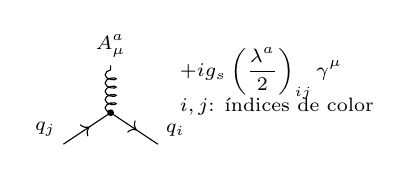
\begin{tikzpicture}[scale=0.4, baseline=(current bounding box.center)]
    % Líneas de Fermiones (Quarks)
    \draw[fermion] (-1.5,-1) node[above left]{$q_j$} -- (0,0);
    \draw[fermion] (0,0) -- (1.5,-1) node[above right]{$q_i$};
    
    % Línea de Bosón (Gluón)
    \draw[gluon] (0,0) -- (0,1.5) node[above]{$A_\mu^a$};
    
    % Punto del Vértice
    \node[vertex] at (0,0) {};
    
    % Factor del Vértice (Etiqueta lateral)
    \node[right] at (1.95, 1.25) {$\displaystyle +ig_s \left( \frac{\lambda^a}{2} \right)_{ij} \gamma^\mu$}; 

    \node[right] at (1.95, 0.20) {$i,j$: índices de color};
\end{tikzpicture}
\end{center}
\vspace{-5pt}
\section{REGLAS DE FEYNMAN}
$\bullet$ \textbf{Propagadores:} Quark: $i\frac{(\cancel{p}+m)}{(p^2-m^2+i\epsilon)} \cdot \delta_{ij}$ \quad  \text{Gluón (Feynman):} $-i\eta_{\mu\nu}\frac{\delta^{ab}}{k^2}$. \\
$\bullet$ \textbf{Vértice Quark-Gluón:} $ig_s  (\frac{\lambda}{2}^a)_{ij}\gamma^\mu$. \\
$\bullet$ \textbf{Vértice 3-Gluones:} $-g_s f^{abc} [\eta_{\mu\nu}(k_1-k_2)_\rho + \eta_{\nu\rho}(k_2-k_3)_\mu + \eta_{\rho\mu}(k_3-k_1)_\nu]$. \\
$\bullet$ \textbf{Vértice 4-Gluones:} $-ig_s^2 [f^{abe}f^{cde}(\eta_{\mu\rho}\eta_{\nu\sigma}-\eta_{\mu\sigma}\eta_{\nu\rho}) + f^{ace}f^{bde}(\eta_{\mu\nu}\eta_{\rho\sigma}-\eta_{\mu\sigma}\eta_{\nu\rho}) + f^{ade}f^{bce}(\eta_{\mu\nu}\eta_{\rho\sigma}-\eta_{\mu\rho}\eta_{\nu\sigma})]$.

\section{CONSTANTES Y SUMAS DE COLOR (SU(3))}

$$C_F\!=\! \frac{N_c^2-1}{2N_c}\!=\!\frac{4}{3}\;\;\;\;C_A\!\!=\! N_c \!=\! 3\;\;\;\;T_F\!=\! \frac{1}{2}$$


$$\delta_{ab}C_A = \sum_{c,c'} f^{acc'}f^{bcc'}\quad \delta_{ij} C_F = \sum_{a,k}\frac{\lambda^a_{ik}}{2}\frac{\lambda^a_{kj}}{2}\quad\delta_{ab}T_F = \sum_{ij} \frac{\lambda^{a}_{ji}}{2} \frac{\lambda^{b}_{ij}}{2}$$



\section{HARD SCATTERING (LÍMITE ULTRARELATIVISTA $m \to 0$)}
Secciones eficaces promediadas ($\sum | \mathcal{M} |^2$) en QCD mediante comparación con QED: \\
$\bullet$ \textbf{$qq' \to qq'$ ($q \neq q'$):} Canal $t$. \quad 
$|\overline{\mathcal{M}}|^2 = \frac{2}{9} [2g_s^4 \frac{s^2+u^2}{t^2}]$. \\
$\bullet$ \textbf{$q\bar{q} \to q'\bar{q}'$ ($q \neq q'$):} Canal $s$.\quad
$|\overline{\mathcal{M}}|^2 = \frac{2}{9} [2g_s^4 \frac{t^2+u^2}{s^2}]$. \\
$\bullet$ \textbf{Bhabha ($q\bar{q} \to q\bar{q}$):} Canales $s$ y $t$. \quad $|\overline{\mathcal{M}}|^2 = 2g_s^4 [\frac{2}{9}\frac{u^2+t^2}{s^2} + \frac{2}{9}\frac{s^2+u^2}{t^2} - \frac{4}{27}\frac{u^2}{st}]$. \\
$\bullet$ \textbf{Compton QCD ($gq \to gq$):} Canales $s, u, t$ \quad
$|\overline{\mathcal{M}}|^2 = g_s^4 [\frac{s^2+u^2}{t^2} - \frac{4}{9}\frac{s^2+u^2}{su}]$. \\
$\bullet$ \textbf{$gg \to gg$:} $|\overline{\mathcal{M}}|^2 = \frac{9}{2} g_s^4 [3 - \frac{ut}{s^2} - \frac{st}{u^2} - \frac{su}{t^2}]$.

\section{CÁLCULO DE FACTORES DE COLOR ($F_c$)}
Procedimiento: extraer tensores de color de $\mathcal{M}$ y $\mathcal{M}^*$, promediar iniciales y sumar finales. \\
$\bullet$ \textbf{Promedio inicial:} $\frac{1}{N_{c1} N_{c2}}$ (Quarks: 3, Gluones: 8). \\
$\bullet$ \textbf{Ejemplo $qq' \to qq'$:} \quad $F_C =  \frac{1}{3 \cdot 3} \sum_{\substack{ijkm \\ a ba'b'}} (t^a_{ij}\delta_{ab}t_{km}^b)(t^{a'*}_{ij}\delta_{a'b'}t_{km}^{b'*})\!=\!\hspace{-5pt}\begin{array}{cc}
     \text{Hermiticidad}\\
      \text{+ props. $\delta_{ab}$}
\end{array} \hspace{-5pt}=$ \\
$= \frac{1}{9} \sum_{ijkm\,ab} (t_{ij}^a t_{km}^a)(t_{ji}^{a'}t_{mk}^{a'}) = \frac{1}{9} \sum_{a a'}\sum_{ij}(t_{ij}^a t_{ji}^{a'})\sum_{km}(t_{km}^a t_{mk}^{a'}) = \begin{array}{cc}
     \text{suma}\\
      \text{de color}
\end{array} = $\\
$=\frac{1}{9} \sum_{a a'}(T_F \delta_{aa'})(T_F \delta_{aa'})=\frac{1}{9} T_F^2 \sum_{a }\delta_{aa}^2 = \frac{1}{9}\cdot 8 \cdot T_F^2 = \frac{2}{9}$
\\
$\bullet$ \textbf{Patas con Quark y/o Fotones:} Incluir delta de color aunque el vértice no sea de QCD. \\
$\bullet$ \textbf{Procesos Mixtos:} $e^+e^- \to q\bar{q}$: $F_c = 3$ \quad  $\gamma q \to \gamma q$: $F_c = 1$ \quad $g q \to \gamma q$: $F_c = \frac{1}{6}$.

\section{QCD EN COLISIONADORES $e^+e^-$ Y COLISIONADORES HADRÓNICOS}
Los partones producidos en el estado final se confinan formando \textbf{jets}. La configuración cinemática típica en colisión frontal cumple $p_{j_1} + p_{j_2} + \dots = 0$.

\textbf{Producción de 2 jets}: $\sigma$($e^-e^+ \to$ 2 jets) $\approx \sum_q \sigma(e^+e^- \to q \bar{q})$. Mediante comparación con $e^+e^- \to \mu^- \mu ^+$, se obtiene para $e^+e^- \to q \bar{q}$:
$$|\overline{F}|^2 = e^4 Q_q^2 N_c \frac{t^2+u^2}{s^2}$$
 $$\sigma(e^-\!e^+\! \to \!q\bar{q}) \!=\! \frac{4\pi\alpha^2}{3s} (Q_q^2 N_c) \!=\! \sigma(e^-\!e^+\! \to\! \mu^-\!\mu^+\!)(Q_q^2 N_c) \quad \frac{\sigma(e^-\!e^+\! \to\! \text{2 jets})}{\sigma(e^-\!e^+\! \to\! \mu^-\!\mu^+)} \!=\! N_c\! \sum_q Q_q^2$$
\\ $\bullet$ $\sum_q$ depende de $\sqrt{s} = 2E$:\;  $\sqrt{s} = [5, 20, 10^3]$ GeV $\to q: [u\,d\,s\,c,\; u\,d\,s\,c\,b, \; u\,d\,s\,c\,b\,t]$


\textbf{Producción de 3 jets:} ($e^-e^+ \to$ 3 jets) $\approx \sum_q \sigma(e^-e^+ \to q\bar{q}g)$. El factor de color es constante para las contribuciones.
$F_c = \sum_{\alpha, i, j} t_{ij}^\alpha t_{ji}^\alpha = C_F \cdot N_c = \frac{4}{3} \cdot 3 = 4$

Definiendo las fracciones de energía del centro de masas para los partones finales $x_i = \frac{2E_i}{\sqrt{s}}$ sujeto a la restricción cinemática $x_1+x_2+x_3=2$, la ratio diferencial es:
$$\frac{\sigma(e^-e^+ \to 3\text{ jets})}{\sigma(e^-e^+ \to 2\text{ jets})} = \frac{2\alpha_s}{3\pi} \iint \frac{x_1^2+x_2^2}{(1-x_1)(1-x_2)} dx_1 dx_2\qquad \alpha_s = \frac{g_s^2}{4\pi}$$

\textbf{Colisón de hadrones ($pp$ o $p\bar{p}$):}  los partones no son elementales. Intervienen \underline{\text{PDFs}} en el estado inicial y \underline{\text{funciones de hadronización}} en el final.

$\bullet$ \text{Teorema de Factorización:}
La sección eficaz hadrónica total es la convolución de las PDFs con la sección eficaz partónica (\textit{hard scattering process}):
$$\sigma(pp \to X) = \sum_{i,j} \int_0^1 dx_1 \int_0^1 dx_2 \, f_i(x_1, Q^2) f_j(x_2, Q^2) \hat{\sigma}_{ij}(\hat{s}) + (x_1 \leftrightarrow x_2)$$
\\ $\bullet$ $f_{i/j}(x, Q^2)$: prob hallar partón $i/j$ con fracción de momento $x$ evaluado a energía $Q^2$.
\\ $\bullet$ $\hat{\sigma}_{ij}$: Sección eficaz a nivel de partones (ej. $q\bar{q} \to q'\bar{q}'$). Dominado por QCD: $\hat{\sigma} \sim \mathcal{O}(\alpha_s^2)$.
\\ $\bullet$ $\hat{s}= x_1 x_2 s$: Invariante de Mandelstam partónico. Se asume típicamente $Q^2 = \hat{s}$.
\\ $\bullet$ Suma contribuciones a nivel de sección eficaz (no de amplitud, $\nexists$ interferencia macro).\\
$\bullet$ \textbf{Aproximación Valencia:} Hadrón $H$ compuesto por $n_v$ quarks de valencia, PDF para quark $i$: 
$q_{v,i}(x, Q^2) = n_i \delta\left(x - \frac{1}{n_v}\right)$, con $n_i$ quarks de valencia de sabor $i$ en $H$.




\section{FAMILIAS DE FERMIONES}

{
\centering
\begin{tabular}{c|c|c}
\textbf{1ª familia} & \textbf{2ª familia} & \textbf{3ª familia} \\
\hline
$\binom{\nu_{eL}}{e_L^-}, e_R^-$ & $\binom{\nu_{\mu L}}{\mu_L^-}, \mu_R^-$ & $\binom{\nu_{\tau L}}{\tau_L^-}, \tau_R^-$ \\
$\binom{u_L}{d_L}, u_R, d_R$ & $\binom{c_L}{s_L}, c_R, s_R$ & $\binom{t_L}{b_L}, t_R, b_R$
\end{tabular}

\vspace{5pt}

\begin{tabular}{c|c|c|c|c|c|c|c}
\hline
& $u_R$ & $u_L$ & $d_R$ & $d_L$ & $\nu_{eL}$ & $e_R$ & $e_L$ \\
\hline
$Y$ & $4/3$ & $1/3$ & $-2/3$ & $1/3$ & $-1$ & $-2$ & $-1$ \\
\hline
$T_3$ & $0$ & $1/2$ & $0$ & $-1/2$ & $1/2$ & $0$ & $-1/2$ \\
\hline
$Q$ & $2/3$ & $2/3$ & $-1/3$ & $-1/3$ & $0$ & $-1$ & $-1$
\end{tabular}

\vspace{3pt}

}

Para la 2ª y 3ª familia es idéntico, con: $[u, \, d,\, e, \, \nu_e] \to [c, \, s, \, \mu, \nu_\mu] \to [t, \, b, \, \tau, \, \nu_\tau] $



\section{SIMETRÍA ELECTRODÉBIL (SM-EW): $SU(2)_L \times U(1)_Y$}
$\bullet$ \textbf{Quiralidad}: $\Psi_{L,R} = P_{L,R}\Psi$, con proyectores $P_{L,R} = \frac{1 \mp \gamma_5}{2}$.
\\ $\bullet$ \textbf{Generadores}: Para $SU(2)_L$, $T_i = \frac{\sigma_i}{2}$ (Isospín débil). Para $U(1)_Y$, hipercarga débil $Y$.
\\ $\bullet$ \textbf{Fermiones}: Agrupados en dobletes levógiros $L$ y singletes dextrógiros $R$.
\\ $\bullet$ \textbf{Carga eléctrica}: Relaciones: $Q = T_3 + \frac{Y}{2} \quad J_{\rm EM }^\mu = J_3 ^\mu + \frac{1}{2} J_{\rm Y}^\mu$.\\


$\bullet$ \textbf{Derivada covariante:} $D_\mu = \partial_\mu - igT_a W_\mu^a - ig'\frac{Y}{2}B_\mu$\\
$\bullet$ $W_\mu^a$ ($a=1,2,3$) bosones de gauge de $SU(2)_L$ con acoplo $g$. 
\\ $\bullet$ $B_\mu$ bosón de gauge de $U(1)_Y$ con acoplo $g'$.
\\ $\bullet$ \textbf{Bosones físicos}: Mezcla de $W_\mu^3$ y $B_\mu$ parametrizada por el ángulo débil $\theta_w$.
$$W_\mu^\pm = \frac{1}{\sqrt{2}}(W_\mu^1 \mp iW_\mu^2) \quad Z_\mu = W_\mu^3\cos\theta_w - B_\mu\sin\theta_w \quad A_\mu = W_\mu^3\sin\theta_w + B_\mu\cos\theta_w$$ 
$\bullet$ \textbf{Unificación}: $e = g \sin\theta_w = g' \cos\theta_w$. Para $Q^2= M_Z^2: e = 0.31, \, g = 0.65, \, g' =0.35$
\\ $\bullet$ \textbf{Masas}: Mecanismo de Higgs $M_Z = \frac{M_W}{\cos\theta_w}$; Constante de Fermi $\frac{G_F}{\sqrt{2}} = \frac{g^2}{8M_W^2}$. 

\section{LAGRANGIANO ELECTRODÉBIL}
\vspace{-2mm}
$$\mathcal{L}_{EW} = \sum_f \bar{\Psi}i\cancel{D}\Psi - \frac{1}{4}W_{\mu\nu}^a W_a^{\mu\nu} - \frac{1}{4}B_{\mu\nu}B^{\mu\nu}\;\;\;\;f \equiv \rm fermiones$$
$$W_{\mu\nu}^a = \partial_\mu W_\nu^a - \partial_\nu W_\mu^a + g\epsilon^{abc}W_\mu^b W_\nu^c \qquad B_{\mu\nu} = \partial_\mu B_\nu - \partial_\nu B_\mu$$ 

\section{REGLAS DE FEYNMAN (VÉRTICES)}
$\bullet$ \textbf{Corriente cargada ($W^\pm$)}: Interacciona solo con fermiones $L$. $W^\pm \rightarrow f \bar{f}': \;\; \frac{ig}{\sqrt{2}}\gamma^\mu P_L$
\\$\bullet$ Vértices con quarks: multiplica por elemento matriz CKM ($U_{ij}$) y tensor de color. 

$U_{\text{CKM}} = 
\begin{pmatrix}
|V_{ud} |& |V_{us}| & |V_{ub}| \\
|V_{cd}| & |V_{cs}| & |V_{cb} |\\
|V_{td}| & |V_{ts}| & |V_{tb}|
\end{pmatrix}
=
\begin{pmatrix}
0.974 & 0.224 & 0.00365 \\
0.224 & 0.973 & 0.0421 \\
0.00896 & 0.0413 & 0.999
\end{pmatrix}
\approx \mathbb{I} + 
\begin{array}{cc}
\text{correcciones}  \\
\text{pequeñas} 
\end{array}
$\\
$\bullet$ \textbf{Corriente neutra ($Z^0$)}: Interacciona con $L$ y $R$. $Z^0 \rightarrow f \bar{f}:\;\; \frac{ig}{\cos\theta_w}\gamma^\mu (g_L P_L + g_R P_R)$\\
$\bullet$ Vértices con neutrinos: multiplica por $\frac{1}{2}$ y sustituye la parte entre paréntesis por $P_L$.
\\$\bullet$ Vértices con quarks: multiplica por el tensor de color.

$\bullet$ \textbf{Acoplos quirales del $Z$}: $g_L = T_3 - Q\sin^2\theta_w$, $g_R = -Q\sin^2\theta_w$. 

\section{PROPAGADORES Y ESTADOS EXTERNOS}
$\bullet$ \textbf{Propagador fermión}: $\frac{i(\cancel{p}+m)}{p^2-m^2}$ (multiplicado por el tensor de color para quakrs). 
\\ $\bullet$ \textbf{Propagador bosón $V$ ($W, Z$)}: $\frac{-i(g_{\mu\nu} - k_\mu k_\nu/M_V^2)}{k^2-M_V^2}$. 
\\ $\bullet$ \textbf{Completitud}: Bosones masivos ($k^2 = M_V^2$) con 3 estados de polarización ($\lambda=\pm 1, 0$):
$$\sum_{\lambda} \epsilon_\mu^{(\lambda)}(k) \epsilon_\nu^{(\lambda)*}(k) = -g_{\mu\nu} + \frac{k_\mu k_\nu}{M_V^2} \epsilon_\mu(k) k^\mu = 0$$

\section{CÁLCULO DE AMPLITUDES (TRAZAS)}
$\bullet$ Amplitud cuadrada promediada: $|\overline{\mathcal{M}}|^2 = \frac{1}{\prod s_{in}} \sum |\mathcal{M}|^2$. 
\\ $\bullet$ \textbf{Propiedades trazas}: $P_L P_R = 0$, $P_L^2 = P_L$, $\gamma^\mu P_L = P_R \gamma^\mu$. 

$$\text{Tr}\{\gamma^\mu \gamma^\nu \gamma^\rho \gamma^\sigma\} = 4(g^{\mu\nu}g^{\rho\sigma} - g^{\mu\rho}g^{\nu\sigma} + g^{\mu\sigma}g^{\nu\rho}) \qquad \text{Tr}\{\gamma^\mu \gamma^\nu \gamma^\rho \gamma^\sigma \gamma_5\} = -4i\epsilon^{\mu\nu\rho\sigma}$$ 

$\bullet$ Contracción de tensores de Levi-Civita: $\epsilon_{\alpha\beta\mu\nu}\epsilon^{\rho\sigma\mu\nu} = -2(\delta_\alpha^\rho\delta_\beta^\sigma - \delta_\alpha^\sigma\delta_\beta^\rho)$ 

\section{CINEMÁTICA Y TASAS DE DESINTEGRACIÓN}
$\bullet$ Anchura parcial para desintegración $1 \rightarrow 2$: $\Gamma = \int \frac{1}{2M_W} |\overline{\mathcal{M}}|^2 d\text{Lips}(M_W; p_1, p_2)$\\
$\int d\text{Lips} = \frac{\sqrt{(M^2 - (m_1+m_2)^2)(M^2 - (m_1-m_2)^2)}}{8\pi M^2}$ \;\;si $m_1, m_2 \rightarrow 0 \Rightarrow \int d\text{Lips} = \frac{1}{8\pi}$.

$$d\text{Lips}_2 = (2\pi)^4 \delta^{(4)}(P - p_1 - p_2) \frac{d^3p_1}{(2\pi)^3 2E_1} \frac{d^3p_2}{(2\pi)^3 2E_2}\qquad d\text{Lips}_2 = \frac{|\mathbf{p}_f|}{16\pi^2 M} d\cos\theta \, d\phi$$

$\bullet$ \textbf{Sección eficaz}: $\frac{d\sigma}{d\Omega_{cm}} = \frac{1}{64\pi^2 s} |\overline{\mathcal{M}}|^2 \frac{|\mathbf{p}_f|}{|\mathbf{p}_i|}$. 


\section{ANCHURAS DE DESINTEGRACIÓN (W y Z)}
\textbf{Decaimiento del Bosón W:}
\\ $\bullet$ $\Gamma(W^- \to d\bar{u}) = 3 |V_{ud}|^2 \Gamma(W^- \to e^- \bar{\nu}_e) = 3 |V_{ud}|^2 ( g^2 M_W / 48\pi ) \;\;\; V_{ud} \overset{U_{CKM\approx 1}}{\approx} 1$
\\ $\bullet$ Factor de color: $F_c = \sum \delta_{ij}\delta_{ij}^* = 3$


\textbf{Decaimiento del Bosón Z:}
\\ $\bullet$ Anchura a neutrinos: $\Gamma(Z \to \nu_e \bar{\nu}_e) = g^2 M_Z/96\pi \cos^2\theta_w$ 
\\ $\bullet$ \textbf{Branching Ratios (BR)} aproximados: 
\\  Invisible ($Z \to \nu\bar{\nu}$): $\sim 20\%$ \;  Hadrónico ($Z \to q\bar{q}$): $\sim 70\%$ \; Leptónico ($Z \to l^+l^-$): $\sim 10\%$ 

\section{NARROW WIDTH APPROXIMATION (NWA)}
\textbf{Modificación del Propagador:} Para partículas inestables en canales $s$.
$$ \frac{1}{k^2 - M^2} \longrightarrow \frac{1}{k^2 - M^2 + i\Gamma M} $$

\textbf{Límite NWA ($\Gamma \ll M$):} Sustitución de la resonancia por la delta de Dirac.
$$ \frac{1}{(s - M^2)^2 + M^2 \Gamma^2} \longrightarrow \frac{\pi}{M\Gamma} \delta(s - M^2) $$ 
\\ $\bullet$ \textbf{Factorización de la Sección Eficaz:} Válido on-shell. $X$ partícula virtual. BR sig. pag. 

$$ \sigma(A+B \to C+D) \approx \sigma(A+B \to X) \cdot \text{BR}(X \to C+D) \quad \text{con } \sigma(A+B\to X) =\frac{\pi}{s}|\bar{F}|^2\delta (s-M_x^2)$$

\section{REGLAS DE FEYNMAN: BOSONES EW}
\textbf{Autointeracciones (Vértices de 3 y 4 puntos):}

% Generados por términos de Yang-Mills $-\frac{1}{4}W_{\mu\nu}W^{\mu\nu} - \frac{1}{4}B_{\mu\nu}B^{\mu\nu}$. % 
$\bullet$ Vértice $W^+ W^- \gamma$ $ -ie \left[ (k_1-k_2)_\lambda g_{\mu\nu} + (k_2-k_3)_\mu g_{\nu\lambda} + (k_3-k_1)_\nu g_{\lambda\mu} \right] $ 
\\ $\bullet$ Estructura tensorial vértices de 4 puntos: $ S_{\mu\nu,\lambda\rho} \equiv 2g_{\mu\nu}g_{\lambda\rho} - g_{\mu\lambda}g_{\nu\rho} - g_{\mu\rho}g_{\nu\lambda} $
\\ $\bullet$ Vértice $W^+ W^- \gamma \gamma$: $-i e^2 S_{\mu\nu,\lambda\rho}$ 

\section{BOSÓN DE HIGGS}
Escalar (Spin = 0), neutro, sin color. Propagador: $\frac{i}{p^2 - M_H^2}$ 

\textbf{Vértices de Interacción:} Los acoplamientos crecen con la masa de la partícula.
\\ $\bullet$ $H W^+ W^-$: $ig M_W g_{\mu\nu}$ \qquad $\bullet$ $H Z Z$: $\frac{ig M_Z}{\cos\theta_w} g_{\mu\nu}$ \qquad $\bullet$ $H f \bar{f}$ (Fermiones): $-i \frac{g}{2} \frac{m_f}{M_W} \delta_{ij}$ 

\textbf{Desintegración a Fermiones ($H \to f\bar{f}$):} 
\\ $\bullet$ Amplitud promediada (ej. $H \to b\bar{b}$): $|\overline{F}|^2 = 3 \frac{g^2 m_b^2}{4 M_W^2} \text{Tr}[(p_1+m_b)(p_2-m_b)]$ 
\\ $\bullet$ Anchura parcial dominante ($H \to b\bar{b}$): 
$$ \Gamma = \frac{3}{32\pi} \frac{g^2 m_b^2 M_H}{M_W^2} \left(1 - \frac{4m_b^2}{M_H^2}\right)^{3/2} $$ 
\\ $\bullet$ Branching Ratio principal: $\text{BR}(H \to b\bar{b}) \approx 60\%$ 



\hrule

\section{CINEMÁTICA Y DISPERSIÓN \normalfont{\quad $E^2 = p^2 + m^2, \quad p^2 = \vec{p}\cdot\vec{p}, \quad p_i^2 = m_i^2$}}
$\bullet$ \textbf{Desintegración $A \rightarrow B+C$ en CM} -- Condición: $m_A \geq m_B + m_C$\\
$|\vec{p}_B|^2\!= \!|\vec{p}_C|^2\! = \!|\vec{p}_f|^2 \!=\! \frac{m_A^2+m_B^2 +m_C^2 - 2m_A^2m_B^2 - 2m_A^2 m_C^2 - 2m_B^2 m_C^2}{4m_A^2}\!\! = \!\!\frac{\lambda(m_A, m_B, m_C)}{4m_A^2}$\\
$\lambda:$ Función de Källén \quad $E_B = \frac{m_A^2 + m_B^2 - m_C^2}{2m_A}$ \quad $E_C = \frac{m_A^2 + m_C^2 - m_B^2}{2m_A}$\\
$$ \textbf{Anchura de Desintegración Diferencial:}  \quad d \Gamma = \frac{1}{2m_A} |\bar{F}|^2 \, d{Lips}(m_A^2, p_B, p_C) $$
$$ d{Lips}(m_A^2, p_B, p_C) = (2\pi)^4 \delta^4(p_A - p_B - p_C) \frac{d^3\vec{p}_B}{(2\pi)^3 2E_B} \frac{d^3\vec{p}_C}{(2\pi)^3 2E_C} = \frac{1}{16\pi^2} \frac{|\vec{p}_f|}{m_A} d\Omega $$
$$ \textbf{Promedio de spin:}\quad|\bar{F}|^2 = \frac{1}{2S_A+1} \sum_{s_A, s_B, s_C} |F|^2 $$
$$ \frac{d\Gamma}{d\Omega} = \frac{1}{32\pi^2} \frac{|\vec{p}_f|}{m_A^2} |\bar{F}|^2 $$
\\
$\cdot$ If {$m_B = m_C = m$} $\rightarrow$ $m_A \eqqcolon M$ \quad $|\vec{p}_f|^2 = \frac{M^2}{4} \left(1-\frac{4m^2}{M^2}\right)$ \quad $E_f = \frac{M}{2}$

$\bullet$ \textbf{Desintegración $1+2 \rightarrow 3+4$ en CM (en canal $s$)} -- Conditions: \hspace{-5pt}$\begin{array}{cc}
     \sqrt{s} \!=\!E_{\rm CM}\!\geq\! m_1 \!+\!m_2 \\
      \sqrt{s} \!=\!E_{\rm CM} \!\geq \!m_3 \!+\! m_4
\end{array}$\\

$$|\vec{p}_i| = \frac{\sqrt{\lambda (s, m_1^2, m_2^2)}}{2\sqrt{s}} \qquad |\vec{p}_f| = \frac{\sqrt{\lambda (s, m_2^3, m_4^2)}}{2\sqrt{s}}  \quad m_1 =m_3 \;\; \& \;\; m_2=m_4 \Rightarrow |\vec{p}_i| = |\vec{p}_f| $$

$$E_1 = \frac{s + m_1^2 - m_2^2}{2\sqrt{s}} \quad  E_2 = \frac{s + m_2^2 - m_1^2}{2\sqrt{s}} \quad E_3= \frac{s + m_3^2 - m_4^2}{2\sqrt{s}} \quad E_4 = \frac{s + m_4^2 - m_3^2}{2\sqrt{s}} \quad $$

 $\bullet$ \textbf{Ataque $1$ contra $2\rightarrow 3+4$}: $s_{\min} = (m_3 +m_4)^2$ \; i.e. salida en reposo\\
$\cdot$ \textbf{LAB}: $E_{\text{lab}} = E_1 = \frac{s-m_1^2 - m_2^2}{2m_2}\quad p_\text{lab} = \frac{\sqrt{\lambda(s,m_1^2, m_2^2)}}{2m_2}$ \\
 $\cdot$ \textbf{CM}:\, \, $E_{1,2} = \frac{m_{1,2}^2+m_2\cdot E_{\text{lab}} }{\sqrt{s}}\quad\; p_{1,2} = p_{\text{lab}}\frac{m_2}{\sqrt{s}}$



\section{PROBABLIDAD DE TRANSICIÓN Y BRANCHING RATIO}
$\bullet$ \textbf{Probabilidad de Transición:} $\mathcal{P}_{i \to f}(t) = \left| \langle \psi_f | \hat{U}(t, 0) | \psi_i \rangle \right|^2$

 $\bullet$ $\hat{U}(t, 0) \equiv$ operador de evolución temporal. Si $\hat{H} \neq \hat{H}(t) \Rightarrow \hat{U}(t, 0) = e^{-i \hat{H} t}$.


$\bullet$ \textbf{Branching Ratio:} Let $A \rightarrow bc$, $BR \,(A\rightarrow bc)= \frac{\Gamma(A\rightarrow bc)}{\Gamma_{\rm tot} (A)}$, $\Gamma\equiv$ anchura desintegración. 

$\bullet$ $BR \,(A\rightarrow bc):$ probabilidad de $A$ de decaer a $bc$.

$\bullet$ En el límite de conservación exacta de I: $\Gamma(A \rightarrow bc) \propto |\langle A|bc \rangle| ^2  = C.G.^2$

\section{ISOSPIN SU(2) EN FORMA MATRICIAL}

\section*{Rep. Fundamental ($I=1/2$) -- \normalfont{Base:  $\{\ket{\frac{1}{2}, \frac{1}{2}} , \ket{\frac{1}{2}, -\frac{1}{2}}\}$. $I_a = \frac{\sigma_a}{2}$ }  = $\{\left(\begin{smallmatrix}
    1\\
    0
\end{smallmatrix}\right), \left(\begin{smallmatrix}
    0\\
    1
\end{smallmatrix}\right)\} $}
$
I_1 = \frac{1}{2} \left(\begin{smallmatrix} 0 & 1 \\ 1 & 0 \end{smallmatrix}\right) \quad
    I_2 = \frac{1}{2} \left(\begin{smallmatrix} 0 & -i \\ i & 0 \end{smallmatrix}\right) \quad
    I_3 = \frac{1}{2} \left(\begin{smallmatrix} 1 & 0 \\ 0 & -1 \end{smallmatrix}\right) \quad
    I_+ = \left(\begin{smallmatrix} 0 & 1 \\ 0 & 0 \end{smallmatrix}\right) \quad
    I_- = \left(\begin{smallmatrix} 0 & 0 \\ 1 & 0 \end{smallmatrix}\right)
$


\section*{Rep. Adjunta ($I=1$) -- \normalfont{Base: $\{\ket{1, 1}, \ket{1, 0}, \ket{1, -1}\}$ = $\{\left(\begin{smallmatrix}
    1\\
    0\\
    0
\end{smallmatrix}\right), \left(\begin{smallmatrix}
    0\\
    1\\
    0
\end{smallmatrix}\right),
\left(\begin{smallmatrix}
    0\\
    0\\
    1
\end{smallmatrix}\right)\}$}}
$
    I_1 \!=\! \frac{1}{\sqrt{2}} \left(\begin{smallmatrix} 0 & 1 & 0 \\ 1 & 0 & 1 \\ 0 & 1 & 0 \end{smallmatrix}\right) \;
    I_2 \!=\! \frac{1}{\sqrt{2}} \left(\begin{smallmatrix} 0 & -i & 0 \\ i & 0 & -i \\ 0 & i & 0 \end{smallmatrix}\right) \;
     I_3 \!=\! \left(\begin{smallmatrix} 1 & 0 & 0 \\ 0 & 0 & 0 \\ 0 & 0 & -1 \end{smallmatrix}\right)  \;
     I_+ \!=\! \sqrt{2} \left(\begin{smallmatrix} 0 & 1 & 0 \\ 0 & 0 & 1 \\ 0 & 0 & 0 \end{smallmatrix}\right) \;
    I_- \!=\! \sqrt{2} \left(\begin{smallmatrix} 0 & 0 & 0 \\ 1 & 0 & 0 \\ 0 & 1 & 0 \end{smallmatrix}\right)
$



\section{ACOPLAMIENTO DE ISOSPINES}
$\bullet$ \underline{Degeneración:} Sistema $N\geq 3$ partículas, $(I, I_3)$ degenerados $\rightarrow$ especifica acoplamientos intermedios (ej. $I_{12}$ para el subsistema $1+2$), y $\langle I_{12}; I, I_3 | I'_{12}; I, I_3 \rangle = \delta_{I_{12} I'_{12}}$ 


$\bullet$ \underline{Regla de Selección si $I_3 = 0$:}
$\langle i_1, 0; i_2, 0 | I, 0 \rangle = 0 \quad \text{si } (i_1 + i_2 - I) \text{  impar.}$

$\therefore$ Si 2 partículas $=$ multiplete ($i_1 = i_2 = i$) $\Rightarrow$ $I \in 2 k, \,\; k \in \mathbb{N}$.

$\therefore$ Si conservación isospín $\Rightarrow$ $I$ inicial impar: prohibido decay en 2 partículas con $I_3 = 0$.

$\bullet$ \underline{Elemento neutro:}  $|0, 0\rangle$: $|j, m\rangle \otimes |0, 0\rangle = |j, m\rangle$ 


\section{CRITERIOS EXTRA CONSERVACIÓN}
$\bullet$ Los sistemas de partículas deben cumplir la antisimetría fermiónica o simetría bosónica iff todas las partículas son idénticas. En caso contrario, no están constreñidas por simetría.

$\bullet$ \textbf{Teorema Landau-Yang}: Partícula vectorial (spin = 1) no puede decaer a 2$\gamma$ o 2 gluones.

$\bullet$ $L \in \mathbb{N} \;\; \forall$ sistema de partículas. 







\hypertarget{quarks_table}{\section{QUARKS (CHARM, BOTTOM, TOP)}}
\begin{center}
\begin{tabular}{|c|c|c|c|c|c|c|c|c|c|}
\hline
\textbf{q} & \textbf{$Q$} & \textbf{$T_3$} & \textbf{$Y$}  & \textbf{$C$} & \textbf{$\scalebox{0.80}{${\tilde{B}}$}$} & \textbf{$T$} & \textbf{$B$} & \textbf{spin}\\ \hline
$c$ & $+2/3$ & $0$ & $+4/3$  & $+1$ & $0$ & $0$ & $1/3$ & $1/2$ \\ \hline
$b$ & $-1/3$ & $0$ & $-2/3$  & $0$ & $-1$ & $0$ & $1/3$ & $1/2$ \\ \hline
$t$ & $+2/3$ & $0$ & $+4/3$  & $0$ & $0$ & $+1$ & $1/3$ & $1/2$ \\ \hline
\end{tabular}\\[2pt]
Antiquarks: todos los números $Q, T_3, Y,  C, \tilde{B}, T, B$ opuestos.
\end{center}


\section{EXPRESIONES ÚTILES y CRITERIOS EN QED}
$dLIPS$ carece de sentido fuera de una integral. La delta de Dirac consume un diferencial para devolver el valor de la función en el punto de la ligadura:$$\int f(\vec{p}_4) \delta^{(3)}(\vec{p}_{\rm total} - \vec{p}_3 - \vec{p}_4) d^3 p_4 = f(\vec{p}_{\rm total} - \vec{p}_3)$$


$\bullet$ Diffs: $d^3 p_k \!=\! d^3 |\vec{p}_k|\!=\!|\vec{p}_k|^2\, d|\vec{p}_k| \, d\Omega\quad d\Omega \!=\! d(\cos\theta)d\varphi\quad \Omega \!=\! \int_{0}^{2\pi} \int_{0}^{\pi} \sin \theta \, d\theta \, d\varphi\! =\! 4\pi$
\vspace{4pt}

En el caso $1+2 \rightarrow 3+4, \;\; \theta \equiv$ ángulo entre 1 y 3. \qquad $dt = 2 |\vec{p}_{\rm in}||\vec{p}_{\rm out}| d(\cos \theta)$

$\bullet$ Källen: $\lambda(x,y,z) = x^2+y^2+z^2-2xy-2xz-2yz \quad \lambda(A,B,B)=A(A-4B^2)$


\textbf{CÁLCULO AMPLITUD (VERSIÓN EXTENDIDA)}

\underline{\textit{1. Patas Externas}}: Líneas externas con cuadrimomento $p$ y espín/helicidad $s$ o $\lambda$.

{

\centering
\begin{tabular}{llcc}
\hline
\textbf{Partícula} & \textbf{Espín} & \textbf{Entrante} & \textbf{Saliente} \\
\hline
Escalar       & 0   & $1$                        & $1$                         \\
Fermión       & 1/2 & $u(p,s)$                   & $\bar{u}(p,s)$              \\
Antifermión   & 1/2 & $\bar{v}(p,s)$             & $v(p,s)$                    \\
Fotón         & 1   & $\epsilon^\mu(p,\lambda)$  & $\epsilon^{*\mu}(p,\lambda)$\\
\hline
\end{tabular}


}

\vspace{2pt}

\underline{\textit{2. Propagadores (Líneas Internas)}}: Líneas que transportan un cuadrimomento $q$. 

\textit{Nota sobre el término $+i\epsilon$:} La prescripción $+i\epsilon$ desplaza los polos fuera del eje real para respetar la causalidad al integrar sobre $d^4q$. En diagramas a nivel árbol, $q$ está unívocamente determinado por la conservación en los vértices, no hay integración, y el término $+i\epsilon$ se puede omitir. En diagramas de lazos, es estrictamente necesario.
\vspace{-0.5mm}
{
$$\begin{array}{ccc}
\hline
\text{Escalar} & \text{Fermión de Dirac} & \text{Fotón (Gauge de Feynmann, } q=k) \\
\hline
\frac{i}{q^2 - m^2 + i\epsilon} & \frac{i(\cancel{q} + m)}{q^2 - m^2 + i\epsilon} & \frac{-ig_{\mu\nu}}{q^2 + i\epsilon} \\
\hline
\end{array}$$

}
\vspace{2pt}
\underline{\textit{3. Vértices de Interacción}}
Cada vértice impone conservación de cuadrimomento y acopla las partículas. Los índices libres del vértice ($\mu, \nu$) deben estar arriba o abajo indistintamente, pero su contracción con el propagador fotónico ($g_{\mu\nu}$) asegurará la invariancia Lorentz final. Cada vértice tiene índices distintos. ($\phi\equiv $ Escalar)

{

\centering
\begin{tabular}{lc}
\hline
\textbf{Interacción} & \textbf{Vértice} \\[2pt]
$l\bar{l}\gamma$ (QED espinorial, leptones) & $-ieQ_l\gamma^\mu$      \\[2pt]
$q\bar{q}\gamma$ (QED, quarks) & $-iQ_q e\gamma^\mu\delta_{ab}$ \\[2pt]
$\phi\phi\gamma$ (QED escalar). $Q_\phi$ carga de partícula $p_{\rm in}$ & $-iQ_\phi(p_{\text{in}} + p_{\text{out}})^\mu $\\[2pt]
$\phi\phi\gamma\gamma$ (QED escalar) & $2iq^2 g^{\mu\nu}$  \\[2pt]
$\phi^4$ (Autointeracción escalar) & $-i\lambda$ \\[2pt]
$\bar{\psi}\psi\phi$ (Interacción de Yukawa) & $-iy$ \\[2pt]
$q\bar{q}g$ (QCD, interacción no abeliana) & $-ig_s \gamma^\mu (t^c)_{ab}$ \\[2pt]
$f\bar{f}Z$ (Electrodébil, corriente neutra leptones) & $\frac{-ig_w}{2\cos\theta_W}\gamma^\mu(c_V - c_A\gamma^5)$ \\[2pt]
$q\bar{q}Z$ (Electrodébil, corriente neutra quarks) & $\frac{-ig_w}{2\cos\theta_W}\gamma^\mu(c_V^q - c_A^q\gamma^5)\delta_{ab}$ \\[2pt]
$f\bar{f}'W^\pm$ (Electrodébil, corriente cargada leptones)& $\frac{-ig_w}{2\sqrt{2}}\gamma^\mu(1 - \gamma^5)$ \\[2pt]
$u_i\bar{d}_jW^\pm$ (Electrodébil, corriente cargada quarks) & $\frac{-i g_w}{2\sqrt{2}} V_{ij} \gamma^\mu (1 - \gamma^5) \delta_{ab}$ \\
\hline
\end{tabular}

}


\underline{\textit{4. Algoritmo Paso a Paso para Construir $-i\mathcal{M}=-iF$}}

\textbf{1. Líneas Fermiónicas (Lectura Inversa):} Recorre las líneas fermiónicas continuas \textbf{en sentido opuesto a las flechas} (el flujo de número fermiónico).

$-$ Inicia con el estado saliente (ej. $\bar{u}$ o $\bar{v}$, vector fila $1 \times 4$).

$-$ Multiplica por los vértices ($\gamma^\mu$) y propagadores ($\cancel{q}+m$) en el orden en que aparecen al ir hacia atrás (matrices $4 \times 4$).

$-$ Termina en el estado entrante (ej. $u$ o $v$, vector columna $4 \times 1$).

\textbf{2. Líneas Bosónicas:}  Las contribuciones de fotones y escalares son escalares tensoriales o números (en sQED todo conmuta). Multiplica los factores correspondientes a estas líneas tras cerrar las cadenas fermiónicas.

\textbf{3. Índices y Conservación:} 
    Asegúrate de que cada propagador fotónico interno contraiga los índices de los vértices que conecta. Impón la conservación del cuadrimomento global ($p_{\text{iniciales}} = p_{\text{finales}}$) si no se ha cancelado previamente por la regla de oro de Fermi.

\underline{\textit{5. Trucos para manipular $-i \mathcal{M}$ (variables de Mandelstam)}}

$$P \!=\! p_1 + p_2 \!=\! p_3 + p_4  \!\Rightarrow\! P^2 \!=\!s \quad Q \!=\! p_1 - p_3 \!=\! p_4 - p_2  \!\Rightarrow\! Q^2 \!=\! t\quad R \!=\! p_1 - p_4 \!=\! p_3 - p_2  \!\Rightarrow\! R^2 \!=\! u$$
\vspace{-0.5mm}
$$(p_1+p_3) \cdot (p_2+p_4) \!=\! (P+R) \cdot (P-R) \!=\! P^2 - R^2 \!=\! s - u$$$$(p_1+p_4) \cdot (p_2+p_3) \!=\! (P+Q) \cdot (P-Q) \!=\! P^2 - Q^2 \!=\! s - t$$$$(p_1-p_2) \cdot (p_4-p_3) \!=\! (Q+R) \cdot (Q-R) \!=\! Q^2 - R^2 \!=\! t - u$$
\vspace{-0.5mm}
$$\text{A saber: }\quad (A+B)_\mu (A-B)^\mu =  (A+B) \cdot (A-B) = A^2 - B^2$$
\vspace{-0.5mm}
\text{El resto de combinaciones, que no son} $(A+B)(A-B),$ \text{ no dan una diferencia pura:}\vspace{1.5mm}
$p_1 \cdot p_2 = \frac{1}{2}(s - m_1^2 - m_2^2) \;\;\; p_1 \cdot p_3 = \frac{1}{2}(m_1^2 + m_3^2 - t)\;\;\; p_1 \cdot p_4 = \frac{1}{2}(m_1^2 + m_4^2 - u)$

$p_3 \cdot p_4 = \frac{1}{2}(s - m_3^2 - m_4^2) \;\;\; p_2 \cdot p_4 = \frac{1}{2}(m_2^2 + m_4^2 - t)\;\;\;  p_2 \cdot p_3 = \frac{1}{2}(m_2^2 + m_3^2 - u)$
\vspace{1.5mm}



\underline{\textit{6. Promedio}} $|\overline{\mathcal{M}}|^2 = \left( \prod_{i \in \text{iniciales}} \frac{1}{g_{\text{espín}, i} \cdot g_{\text{color}, i}} \right) \sum_{\text{all external states}} |\mathcal{M}|^2$

{

\centering
\renewcommand{\arraystretch}{0.5}
\setlength{\tabcolsep}{2pt} 
\begin{tabular}{lcccc}
\toprule
\textbf{Partícula} & \textbf{Espín ($S$)} & \textbf{Estados Espín ($g_{\text{espín}}$)} & \textbf{Estados Color ($g_{\text{color}}$)} \\
\midrule
Escalar (ej. Higgs) & $0$ & $1$ & $1$  \\
Leptón ($e, \mu, \tau$) & $1/2$ & $2$ & $1$  \\
Neutrino ($\nu$)* & $1/2$ & $1$ (levógiro) & $1$  \\
Quark ($u, d, c, s, t, b$) & $1/2$ & $2$ & $3$  \\
Fotón ($\gamma$) & $1$ & $2$ (masa nula) & $1$  \\
Gluón ($g$) & $1$ & $2$ (masa nula) & $8$  \\
Bosones $W^\pm, Z^0$ & $1$ & $3$ (masivos) & $1$ \\
Gravitón ($G$) & $2$ & $2$ (masa nula) & $1$ \\
\bottomrule
\end{tabular}

}

$- $ En vértices E.M., $\gamma$ no transfiere color $\Rightarrow$ suma sobre estados color quarks: $\sum_{i,j} \delta_{ij} = 3$.

$- $ Para desarrollar $|\mathcal{M}|^2$, usa Trucos de Casimir y $\text{Tr}\{\cancel{a} \gamma^\mu \cancel{b} \gamma^\nu\} = a_\alpha b_\beta \text{Tr}\{\gamma^\alpha \gamma^\mu \gamma^\beta \gamma^\nu\}=$ \\
$\quad= 4 (a^\mu b^\nu + a^\nu b^\mu - a\cdot b \, \,\eta^{\mu \nu} )$. Si índices iniciales abajo, resultado índices abajo.

$-$ Cuando multipliques los resultados de las trazas, debes emplear mismo índice.

$- $ Analiza las divergencias (denominador se anula). Busca relación con $\theta$ (Mandelstam).

$ - $ Expresa todo en función de la carga de cada partícula $Q_p$. Útil comparación de procesos.


\newcolumn

\section{REPRESENTACIONES Y REGLAS DE YOUNG}
\hypertarget{young}{En} $SU(3)$, una representación irreducible se etiqueta según sus números de Dynkin $(p,q)$, donde $p$ es el nº de columnas con una sola caja y $q$ es el nº de columnas con dos cajas.

\begin{tabular}{l c c c}
    \textbf{Nombre} & \textbf{Dim} ${(p,q)}$ & \textbf{Diagrama de Young} & \textbf{Índices Tensoriales} \\
    \hline
    Singlete & $\mathbf{1} \ (0,0)$ & $\cdot$ (o columna de 3) & Escalar \\
    Fundamental & $\mathbf{3} \ (1,0)$ & \scalebox{0.6}{$\ydiagram{1}$} & $\psi^i$ (Quark) \\
    Antifundamental & $\bar{\mathbf{3}} \ (0,1)$ & \scalebox{0.6}{$\ydiagram{1,1}$} & $\psi_i \sim \epsilon_{ijk}\psi^{jk}$ (Antiquark) \\
    Simétrica & $\mathbf{6} \ (2,0)$ & \scalebox{0.6}{$\ydiagram{2}$} & $T^{(ij)}$ \\
    Adjunta (Octete) & $\mathbf{8} \ (1,1)$ & \scalebox{0.6}{$\ydiagram{2,1}$} & $A^i_j$ (traceless) \\
    Decuplete & $\mathbf{10} \ (3,0)$ & \scalebox{0.6}{$\ydiagram{3}$} & $T^{(ijk)}$ \\
    \hline
\end{tabular}

\section{Cálculo de Dimensiones}

Para $SU(3)$, la dimensión de una representación $(p,q)$ viene dada por la fórmula:
$$    \text{Dim}(p,q) = \frac{1}{2}(p+1)(q+1)(p+q+2) $$


Alternativamente, usando método de factores sobre el diagrama:
$ \text{Dim} = \prod_{\text{cajas}} \frac{D_N(\text{caja})}{h(\text{caja})} $

$D_N = N + (\text{col} - \text{fila})$ y $h=$ longitud gancho $= 1 + (\text{celdas a la derecha}) + (\text{celdas debajo})
$.

\section{Reglas del Producto Tensorial (Littlewood-Richardson) para computar $A \otimes B$:}
1. Dibuja el diagrama $A$.

2. Llenar las cajas del diagrama $B$ con letras: `a' en la \textit{primera} fila, `b' en la \textit{segunda}, etc.

3. Añadir las cajas de $B$ al diagrama $A$ siguiendo este orden riguroso:

$\bullet$ Añadir todas las `a', luego todas las `b', etc.

$\bullet$ \text{Regla de Simetría:} No puede haber dos letras iguales en la misma \textit{columna}.

$\bullet$ \text{Regla de Forma:} El resultado debe ser siempre un diagrama de Young válido. Sea $\lambda_i$ el número de cajas en la fila $i$, $\lambda_i \ge \lambda_{i+1}$.

$\bullet$ \text{Regla de Permutación de Red (Lattice):} Leyendo las letras añadidas de derecha a izquierda y de arriba a abajo (estilo hebreo), en cualquier punto de la lectura, el número de `a' leídas debe ser $\ge$ número de `b' $\ge$ número de `c'.

4. Eliminar cualquier columna completa de altura $N=3$ (corresponden al singlete antisimétrico $\epsilon_{ijk}$). Eliminar cualquier columna de altura mayor a $N=3$, el diagrama es nulo y se descarta de la suma directa. Si tienes diagramas idénticos (con mismas letras en las mismas cajas) solo se cuenta uno de ellos.


\section*{1. Vértices Elementales del Modelo Estándar}
\begin{tabular}{@{}lll@{}}
\textbf{Sector} & \textbf{Vértice (Interacción)} & \textbf{Mediador(es)} \\
\midrule
\textbf{QED} & $f + \bar{f} \leftrightarrow \gamma$ & Fotón ($\gamma$) \\
\midrule
\textbf{Débil (CC)} & $f_u + \bar{f}_d \leftrightarrow W^+$ & Bosón $W^\pm$  \\
\textbf{Débil (NC)} & $f + \bar{f} \leftrightarrow Z^0$ & Bosón $Z^0$  \\
\midrule
\textbf{QCD} & $q + \bar{q} \leftrightarrow g$ & Gluón ($g$) \\
\textbf{QCD (3-pt)} & $g + g \leftrightarrow g$ & Gluón ($g$)  \\
\textbf{QCD (4-pt)} & $g + g \leftrightarrow g + g$ & Gluón ($g$)  \\
\midrule
 \textbf{EW Gauge (3-pt)} & $W^+ + W^- \leftrightarrow \gamma$ / $W^+ + W^- \leftrightarrow Z^0$ & $\gamma$, $Z^0$ \\
\textbf{EW Gauge (4-pt)} & $W^+ + W^- \leftrightarrow W^+ + W^-$ & $W^\pm$ \\
 & $W^+ + W^- \leftrightarrow Z^0 + Z^0$ / $W^+ + W^- \leftrightarrow \gamma + \gamma$ & $W^\pm$, $Z^0$, $\gamma$  \\
 & $W^+ + W^- \leftrightarrow Z^0 + \gamma$ & $W^\pm$, $Z^0$, $\gamma$ \\
\midrule
\textbf{Yukawa} & $f + \bar{f} \leftrightarrow H$ & Higgs ($H$) \\
\midrule
\textbf{Higgs-Gauge (3-pt)} & $W^+ + W^- \leftrightarrow H$ / $Z^0 + Z^0 \leftrightarrow H$ & $W^\pm$, $Z^0$  \\
\textbf{Higgs-Gauge (4-pt)} & $W^+ + W^- \leftrightarrow H + H$ / $Z^0 + Z^0 \leftrightarrow H + H$ & $W^\pm$, $Z^0$ \\
\midrule
\textbf{Higgs (Auto)} & $H + H \leftrightarrow H$ & Higgs ($H$) \\
\textbf{Higgs (Auto)} & $H + H \leftrightarrow H + H$ & Higgs ($H$) \\
\end{tabular}



\section*{2. Procesos de Dispersión $2 \to 2$ (Canales $s, t, u$ dominantes a nivel árbol)}


{


\centering
\setlength{\tabcolsep}{2pt} 
\begin{tabular}{@{}lllll@{}}
\textbf{Sector / Proceso} & \textbf{Reacción} & \textbf{Fuerza} & \textbf{Mediador} & \textbf{Canales} \\
\midrule
\textbf{Leptónico Puro} \\
Disp de Møller & $e^- + e^- \to e^- + e^-$ & EM, Débil & $\gamma$, $Z^0$ & $t, u$ \\
Disp de Bhabha & $e^+ + e^- \to e^+ + e^-$ & EM, Débil & $\gamma$, $Z^0$ & $s, t$ \\
Aniq. a Leptones & $e^+ + e^- \to \mu^+ + \mu^-$ & EM, Débil & $\gamma$, $Z^0$ & $s$ \\
Disp Compton & $e^- + \gamma \to e^- + \gamma$ & EM & $e^-$ (fermión) & $s, u$ \\
Aniq. a Fotones & $e^+ + e^- \to \gamma + \gamma$ & EM & $e^-$ (fermión) & $t, u$ \\
Disp $\nu_\mu$-$e$ & $\nu_\mu + e^- \to \nu_\mu + e^-$ & Débil (NC) & $Z^0$ & $t$ \\
Disp $\nu_e$-$e$ & $\nu_e + e^- \to \nu_e + e^-$ & Débil & $Z^0$, $W^\pm$ & $t$ ($Z$), $u$ ($W$) \\
\midrule
\textbf{Semileptónico} \\
Disp Inelástica & $e^- + q \to e^- + q$ & EM, Débil & $\gamma$, $Z^0$ & $t$ \\
Drell-Yan & $q + \bar{q} \to l^+ + l^-$ & EM, Débil & $\gamma$, $Z^0$ & $s$ \\
Decay Inverso & $\mu^- + \nu_e \to e^- + \nu_\mu$ & Débil (CC) & $W^\pm$ & $u$ \\
\midrule
\textbf{Fuertes (QCD)} \\
Disp ($\neq$ sabor) & $q + q' \to q + q'$ & Fuerte & $g$ & $t$ \\
Disp ($=$ sabor) & $q + q \to q + q$ & Fuerte & $g$ & $t, u$ \\
Aniq. ($\neq$ sabor) & $q + \bar{q} \to q' + \bar{q}'$ & Fuerte & $g$ & $s$ \\
Disp Bhabha QCD & $q + \bar{q} \to q + \bar{q}$ & Fuerte & $g$ & $s, t$ \\
Aniq. a Gluones & $q + \bar{q} \to g + g$ & Fuerte & $q$ (fermión) & $t, u$ \\
Producción de pares & $g + g \to q + \bar{q}$ & Fuerte & $q$ ($t, u$), $g$ ($s$) & $s, t, u$ \\
Disp Compton QCD & $q + g \to q + g$ & Fuerte & $q$ ($s, u$), $g$ ($t$) & $s, t, u$ \\
Auto-Disp Gluónica & $g + g \to g + g$ & Fuerte & $g$, contacto $4g$ & $s, t, u$ \\
\midrule
\textbf{Sector de Higgs} \\
Higgsstrahlung & $f + \bar{f} \to V + H$ & Débil & $V$ ($W^\pm, Z^0$) & $s$ \\
Fus. de Bosones & $q + q' \to q + q' + H$ & Débil & $V$ ($W^\pm, Z^0$) & $t, u$ ($V \to H$) \\
Fus. de Gluones & $g + g \to H$ & Fuerte, Yukawa & Quarks Top & Efectivo $s$ \\
\end{tabular}


}



\hrule
~\\
Author: \href{https://www.linkedin.com/in/jorge-acebes-hern%C3%A1ndez/}{Jorge Acebes Hernández}. Code: \href{https://github.com/JorgeAcebes/physics-cheat-sheets/tree/main/Altas%20Energ%C3%ADas}{GitHub}. Last revised: \today \hfill\scalebox{0.8}{
\href{https://creativecommons.org/licenses/by-nc/4.0/}{CC BY-NC 4.0}} 
\vfill


\clearpage

\section*{Integrals%
\normalfont\scriptsize{ $(n\in\mathbb{N}_0,m\in\mathbb{Z},\alpha,\beta,\gamma,\delta,\mu,\nu,\sigma,r\in\mathbb{R},x\in\mathbb{R}\cap\mathrm{Dom}_f,\;a,b,z\in\mathbb{C})$}}
\underline{Basic}\\[0pt]
    \hspace*{0.2cm}
    \scalebox{0.785}{$\int (x+\alpha)^rdx \!=\!\frac{(x+\alpha)^{r+1}}{r+1}$\;\;\;\;\;$ \int x(x+\alpha)^rdx \!=\!\frac{(x+\alpha)^{r+1}(rx{+}x{-}\alpha)}{(r{+}1)(r{+}2)}$\;\;\;\;\;$\int a^xdx \!=\!\frac{a^x}{\ln a}$\;\;\;\;\;$\int u\,dv =uv{-}\int v\,du$}\\
\underline{Rational}
    \\[3pt]\hspace*{0.2cm}
        \scalebox{0.785}{$\int \frac{dx}{\alpha x+\beta} =\frac{1}{\alpha}\ln|\alpha x+\beta|$\;\;\;\; \;$\int \frac{dx}{x^2+\alpha^2} =\frac{1}{\alpha}\arctan\frac{x}{\alpha}$\;\;\;\;\;$\int \frac{dx}{x^2-\alpha^2}=\frac{1}{2\alpha}\ln |\frac{x-\alpha}{x+\alpha}|$\;\;\;\;\;$\int \frac{dx}{\alpha^2-x^2} =\frac{1}{2\alpha}\ln|\frac{\alpha{+}x}{\alpha{-}x}|$}\\[3pt]\hspace*{0.2cm}
        \scalebox{0.785}{$\int \frac{dx}{\alpha x^2+\beta x+\gamma} =\frac{2}{\surd({4\alpha\gamma{-}\beta^2})}\arctan\frac{2\alpha x{+}\beta}{\surd({4\alpha\gamma{-}\beta^2)}}$\;\;\;\;\;$\int \frac{dx}{(x{+}\alpha)(x{+}\beta)} =\frac{1}{\beta{-}\alpha}\ln|\frac{\alpha{+}x}{\beta{+}x}|$}\\[2pt]
    \underline{Roots}
    \\[3pt]\hspace*{0.2cm}
        \scalebox{0.785}{$\int\surd(x^2+\alpha^2)=\frac{1}{2}\big[x\surd(x^2+\alpha^2)+\alpha^2\operatorname{arsinh}\frac{x}{|\alpha|}\big]$\;\;\;\;\;$\int\surd(x^2-\alpha^2)=\frac{1}{2}\big[x\surd(x^2-\alpha^2)-\alpha^2\ln|\surd(x^2-\alpha^2)+x|\big]$}
    \\[3pt]\hspace*{0.2cm}
        \scalebox{0.785}{$\int \frac{dx}{\surd{(x^2+\alpha^2)}} ={\operatorname{arsinh}}\frac{x}{|\alpha|}$\;\;\;\;\;$\int \frac{dx}{\surd{(-x^2+\alpha^2)}} ={\arcsin}\frac{x}{|\alpha|}$\;\;\;\;\;$\int\frac{dx}{\surd(x^2-\alpha^2)}=\ln |\surd(x^2-\alpha^2)+x|$}
    \\[3pt]\hspace*{0.2cm}
        \scalebox{0.785}{$\int\!\frac{dx}{x\surd(x^2+\alpha^2)}\!=\!-\!\frac{1}{\alpha}\operatorname{arsinh}\frac{\alpha}{|x|} $\;\;\;\;$\int\!\frac{dx}{x\surd(-x^2+\alpha^2)}\!=\!-\frac{1}{\alpha}\!\ln\frac{|\surd (-x^2+\alpha^2) +\alpha|}{|x|}$\;\;\;\;$\int\!\frac{dx}{x\surd(x^2-\alpha^2)}\!=\! \frac{1}{\alpha}\!\arctan\frac{\surd(x^2-\alpha^2)}{\alpha}$}
    \\[3pt]\hspace*{0.2cm}
        \scalebox{0.785}{$\int \frac{x}{\surd(x^2\pm\alpha^2 )}dx=\surd(x^2\pm \alpha^2)$\;\;\;\;$\int\frac{x}{\surd(-x^2 +\alpha^2)}dx=-\surd(-x^2+\alpha^2)$}
    \\[3pt]\hspace*{0.2cm}
        \scalebox{0.785}{$\int\frac{dx}{(x^2\pm\alpha^2)^{3/2}}=\frac{\pm x}{\alpha^2 \surd(x^2\pm\alpha^2)}$\;\;\;\;$\int\frac{dx}{(-x^2+\alpha^2)^{3/2}}=\frac{x}{\alpha \surd(-x^2+\alpha^2)}$}
    \\[3pt]\hspace*{0.2cm}
        \scalebox{0.785}{$\int\frac{x}{(x^2\pm\alpha^2)^{3/2}}=\frac{-1}{\surd(x^2\pm\alpha^2)}$\;\;\;\;$\int\frac{x}{(x^2\pm\alpha^2)^{3/2}}=\frac{-1}{\surd(x^2\pm\alpha^2)}$}\\[2pt]
\underline{Trigonometric}\;\;\scalebox{0.8}{$(\mu,\nu>0, \; \chi\equiv x\alpha , \; \gamma\equiv \alpha+\beta, \; \delta \equiv \alpha-\beta)$}
     \\[3pt]\hspace*{0.2cm}
        \scalebox{0.785}{$\int \sin x\,dx = -\cos x $\;\;\;\:$\int  \cos x \, dx = \sin  x$\;\;\;\;\;\;\;\;$\int   \frac{dx}{\sin^2 x} = -\cot x $\;\;\;\;\;\;\;$\int   \frac{dx}{\cos^2 x} = \tan x $\;\;\;\;\:\;\;\:$\int \frac{dx}{\tan ^2 x} = -\cot x-x$}
    \\[3pt]\hspace*{0.2cm}
        \scalebox{0.785}{$\int \sinh x\,dx\! =\! \cosh x $\;\;\;\;\:$\int  \cosh x \, dx\!=\! \sinh x$\;\;\;\;\:$\int   \frac{dx}{\sinh^2 x}\! =\! -\coth x $\;\;\;\;\:$\int   \frac{dx}{\cosh^2 x} \!=\! \tanh x $\;\;\;\;\:$\int\frac{dx}{\tanh^2 x}\!=\!-\coth x\!+x$}
    \\[3pt]\hspace*{0.2cm}
        \scalebox{0.785}{$\int \tan x \, dx= -\ln |\cos x|$\;\;\;\;\:$\int \tan^2x\,dx =\tan x{-}x$\;\;\;\;\:$\int\tanh x\, dx=\ln \cosh x$\;\;\;\;\:$\int\tanh ^2 x\, dx=-\tanh x+x$}
    \\[5pt]\hspace*{0.2cm}
        \scalebox{0.785}{$\int \frac{dx}{\sin x} ={-}\ln|\frac{1}{\sin x}{+}\frac{1}{\tan x}|$\;\;\;\;\:\;\;\:$\int \frac{dx}{\cos x} =\ln|\frac{1}{\cos x}{+}\tan x|$\;\;\;\;\:\;\;\:$\int \frac{dx}{\tan x}=\ln|\sin x|$}
    \\[5pt]\hspace*{0.2cm}
        \scalebox{0.785}{$\int \sin^n\alpha x\,dx \!=\!{-}\frac{\sin^{n-1}\chi\,\cos\chi}{n\alpha}{+}\frac{n-1}{n}\int \sin^{n-2}\alpha x\,dx$\;\;\;\;\:$\int \cos^n\alpha x\,dx \!=\!{+}\frac{\cos^{n-1}\chi\,\sin\chi}{n\alpha}{+}\frac{n-1}{n}\int \cos^{n-2}\alpha x\,dx$}
    \\[5pt]\hspace*{0.2cm}
        \scalebox{0.785}{$\int \sin\alpha x\sin\beta x\,dx \!=\!{-}\frac{\sin \gamma x }{2\gamma}{+}\frac{\sin \delta x}{2\delta}$\;\;\;\;\:$\int \cos\alpha x\cos\beta x\,dx \!=\!{+}\frac{\sin \gamma x}{2\gamma }{+}\frac{\sin\delta x}{2\delta}$\;\;\;\;\:$\int \sin\alpha x\cos\beta x\,dx \!=\!{-}\frac{\cos\gamma x}{2\gamma}{-}\frac{\cos\delta x}{2\delta}$}
    \\[4pt]\hspace*{0.2cm}
        \scalebox{0.785}{$\int x\sin\alpha x\,dx =\frac{\sin\chi }{\alpha^2}{-}\frac{x\cos\chi}{\alpha}$\;\;\;\;\:$\int x\cos\alpha x\,dx =\frac{\cos\chi }{\alpha^2}{+}\frac{x\sin\chi}{\alpha}$\;\;\;\;\:$\int x\genfrac{}{}{0pt}{}{\sin^2}{\cos^2}\alpha x\,dx =\mp\frac{2\chi\,\sin 2\chi \, {+}\cos 2\chi \, \mp\, 2\chi^2}{8\alpha^2}$}
    \\[5pt]\hspace*{0.2cm}
        \scalebox{0.77}{$\int \!x\genfrac{}{}{0pt}{}{\sin\alpha x\sin\beta x}{\cos\alpha x\cos\beta x}dx {=}\!\mp\!\frac{x\sin \gamma x}{2\gamma}\!\mp\!\frac{\cos\gamma x}{2\gamma^2}{+}\frac{x\sin \delta x}{2\delta}{+}\frac{\cos\delta x}{2\delta^2}$\;\;\,\,$\int \!x\sin \alpha x \cos \beta x\,dx {=}{-}\frac{x\cos\gamma x}{2\gamma}{+}\frac{\sin \delta x}{2\delta^2}{-}\frac{x\cos\delta x}{2\delta}\!{+}\frac{\sin\gamma x}{2\gamma^2}$}
    \\[5pt]\hspace*{0.2cm}\scalebox{0.8}{\underline{Definite integrals} ($m!! =m(m{-}2)(m{-}4)...$, \; ${-}1!! =0!! =1!! =1$)}
    \\[2pt]\hspace*{0.2cm}
        \scalebox{0.785}{$\int_0^{\pi/2}\! \sin^\mu x\,dx {=}\int_0^{\pi/2}\! \cos^\mu x\,dx\!=\!\frac{1}{2}\!\operatorname{B}(\frac{\mu+1}{2},\frac{1}{2}) {=}\frac{(n-1)!!}{n!!}\!\cdot\!\begin{cases}\frac{\pi}{2}&\hspace{-3pt}\text{if }\mu{=}n\text{ even}\\\;1&\hspace{-3pt}\text{if }\mu {=}n\text{ odd}\end{cases}$\;\;\;\;\;\;$\int_{-1}^{+1} \genfrac{}{}{0pt}{}{\sin(m\pi x)\sin(\tilde{m}\pi x)}{\cos(m\pi x)\cos(\tilde{m}\pi x)}dx \!=\!\delta_{m,\tilde{m}}$}
    \\[5pt]\hspace*{0.2cm}
        \scalebox{0.785}
{$\left.\hspace{-5pt}
\begin{array}{c}
\int_0^\alpha\!\!\genfrac{}{}{0pt}{}{\sin(\frac{m\pi x}{\alpha})\sin(\frac{\tilde{m} \pi x}{\alpha})}{\cos(\frac{m \pi x}{\alpha})\cos(\frac{\tilde{m}\pi x}{\alpha})}dx \!=\!\frac{\alpha}{2}\delta_{m,\tilde{m}}
\vspace{3pt}\\
\text{also valid $m=1/2$}
\end{array}
\right.$\;\;\;$\int_0^\alpha \!\sin(\frac{m \pi x}{\alpha})\cos(\frac{\tilde{m}\pi x}{\alpha})dx\!=\!\begin{cases}\;\;\;\;\;0&\!\!\text{if }m{+}\tilde{m}\text{ even}\vspace{3pt}\\\frac{2m\alpha}{m^2-\tilde{m}^2}\frac{1}{\pi}&\!\!\text{if }m{+}\tilde{m}\text{ odd}\end{cases}$\;\;\;\;$\int_0^\pi\! \genfrac{}{}{0pt}{}{\sin x\,dx =2}{\cos x\,dx =0}$}
    \\[5pt]\hspace*{0.2cm}
        \scalebox{0.785}{$\int_0^\pi \sin^nx\cos^{\tilde{n}}x\,dx =0\ \forall\, \tilde{n}\text{ odd}$\;\;\;\;\;\;$\int_0^{\pi\mu} \genfrac{}{}{0pt}{}{\sin^2\alpha x}{\cos^2\alpha x}dx =\frac{1}{4\alpha}\left[2\pi\alpha\mu\mp\sin(2\pi\alpha\mu)\right]\stackrel{\text{if }\mu =n} =\frac{\pi n}{\alpha}$\;\;\;\;\;$\int_0^\pi \genfrac{}{}{0pt}{}{\sin^3x\,dx =\frac{4}{3}}{\cos^3x\,dx =0}$}
    \\[5pt]\hspace{0.2cm}
        \scalebox{0.785}{$\int_0^{2\pi} \genfrac{}{}{0pt}{}{\sin x}{\cos x}dx =0$\;\;\;\;\;\;$\int_0^{2\pi} \sin x\cos x\,dx =0$\;\;\;\;\;\;$\int_0^{2\pi} \sin^nx\cos^{\tilde{n}} x\,dx =0\text{ if }n,\tilde{n}\text{ not both even}$\;\;\;\;\;\;$\int_0^{2\pi} \genfrac{}{}{0pt}{}{\sin^3x}{\cos^3x}dx =0$}
    \\[5pt]\hspace{0.2cm}
        \scalebox{0.785}{$\int_0^{2\pi} (1{-}\cos x)^n\sin nx\,dx =0$\;\;\;\;\;\;$\int_0^{2\pi} (1{-}\cos x)^n\cos nx\,dx =(-1)^n\frac{\pi}{2^{n-1}}$}\\[5pt]
\underline{Parity}\;\;\;\;\;\;\;\scalebox{0.8}{$\text{ \textit{Even}}: f_e(-x) = f_e(x)$\;\; 
 \scalebox{0.785}{$\int_{-\alpha}^{+\alpha} f_e(x)\,dx =2\int_{0}^{\alpha}f_e(x)\,dx$\hspace{0.15cm}}\;\;\;$\text{ \textit{Odd}}: f_o(-x) = -f_o(x)$ \;\;\scalebox{0.785}{$\int_{-\alpha}^{+\alpha} f_o(x)\,dx =0$}}
    \\[5pt]\hspace{0.2cm}
        \scalebox{0.785}{$f_e  :   \cos x,\;  \cosh x,\;  x^{2n},\;  e^{-x^2} ,\;  |x|,\;  \delta_{ij},\;  \delta(x),\;  \mathbb{R}, \;  1/f_e, \;  f'_o, \; f_e\pm f_e, \;  f_e\cdot f_e, \; f_o\cdot f_o, \; \mathcal{F}\{f_e(x)\} (\xi),...$}
    \\[5pt]\hspace{0.2cm}
    \scalebox{0.785}{$f_o :  \sin x,\; \sinh x,\; x^{2n+1},\; \tan x,\; \operatorname{erf}x,\; \operatorname{sign}x,\;\ln \big(\frac{1+x}{1-x}\big),\; 1/f_o, \; f'_e,\; f_o\pm f_o, \; f_e \cdot f_o, \;\mathcal{F}\{f_o(x)\} (\xi) ,...$}\\[2pt]
\underline{Log/Exp} \; \scalebox{0.75}{$(r\neq-1)$} 
    \\[2pt]\hspace*{0.2cm}
        \scalebox{0.785}{$\int x^r\ln x\,dx =x^{r+1}\left(\frac{\ln x}{r+1}{-}\frac{1}{(r+1)^2}\right)$\;\;\;\;\;\;$\int(\ln x)^n \, dx= (-1)^n \, n!\, x \displaystyle \sum_{k=0}^n \frac{(-\ln x)^k}{k!}$\;\;\;\;\;$\int \frac{dx}{(e^{-x/\alpha}{+}1)} =\alpha\ln(e^{x/\alpha}{+}1)$}
    \\[5pt]\hspace*{0.2cm}
        \scalebox{0.785}{$\int xe^{\alpha x^2}dx =\frac{e^{\alpha x^2}}{2\alpha}$\;\;\;\;\;\;\;\;$\int x^n  e^{\alpha x}dx=e^{\alpha x}\displaystyle\sum_{k=0}^n  \frac{n!\, (-1)^k}{(n-k)!}\frac{x^{n-k}}{\alpha ^{k+1}}$\;\;\;\;\;\;\;\;$\int \frac{e^{\alpha x}}{x^n}dx =\frac{1}{n{-}1}\left({-}\frac{e^{\alpha x}}{x^{n-1}}{+}\alpha\int \frac{e^{\alpha x}}{x^{n-1}}dx\right)$}
    \\[5pt]\hspace*{0.2cm}\scalebox{0.8}{\underline{Definite integrals} ($r-1,\,\alpha>0$\;\;\;$\gamma\equiv$Euler-Mascheroni constant)}
    \\[3pt]\hspace*{0.2cm}
        \scalebox{0.785}{$\int_0^\infty x^re^{-\alpha x^2}dx =\frac{\Gamma\left(\frac{r+1}{2}\right)}{2\alpha^{\frac{r+1}{2}}} =\begin{cases}\frac{(2n{-}1)!!}{2^{n+1}\;\alpha^n}\sqrt{\frac{\pi}{\alpha}} & \text{if }r =2n \vspace{3pt}\\\frac{n!}{2\;\alpha^{n+1}} & \text{if }r =2n{+}1\end{cases}$\;\;\;\;\;}\scalebox{0.785}{\[\begin{array}{ll}&\int_0^\infty e^{-\alpha x^2}dx =\frac{1}{2}\sqrt{\frac{\pi}{\alpha}}\vspace{5pt}\\&\int_0^\infty x^2e^{-\alpha x^2}dx=\frac{1}{4}\sqrt{\frac{\pi}{\alpha^3}}\end{array}\]}
    \\[6pt]\hspace*{0.2cm}
        \scalebox{0.785}{$\int_0^\infty x^re^{-ax}dx =\frac{\Gamma(r{+}1)}{a^{r+1}}\stackrel{\text{if }r =n} =\frac{n!}{a^{n+1}}$ \ {\scriptsize$(r{>}{-}1,\Re(a){>}0)$}\;\;\;\;\;\;\;\;$\int_0^\infty \sqrt{x}e^{-x}dx =\frac{\sqrt{\pi}}{2}$\;\;\;\;\;\;\;\;$\int_0^\infty \frac{x}{e^x{-}1}dx =\frac{\pi^2}{6}$}
    \\[5pt]\hspace*{0.2cm}
        \scalebox{0.785}{$\int_0^\infty e^{-ax^b}dx =a^{-1/b}\Gamma\left(\frac{1}{b}{+}1\right)$ \;\;\;\;\;\;\;\;$\int_{-\infty}^{+\infty} e^{-\alpha x^2{+}\beta x}dx =\sqrt{\frac{\pi}{\alpha }}e^{\frac{\beta^2}{4\alpha }}$\;\;\;\;\;\;\;\;$\int_0^{2\pi} e^{i(m-\tilde{m})\phi}d\phi =2\pi\delta_{m,\tilde{m}}$}
    \\[5pt]\hspace*{0.2cm}
        \scalebox{0.8}{$\int_0^\infty e^{-\alpha x}\sin(\beta x)dx =\frac{\beta}{\alpha^2{+}b^2}$\;\;\;\;\;\;$\int_0^\infty e^{-\alpha x}\cos(\beta x)dx =\frac{\alpha }{\alpha^2{+}\beta^2}$\;\;\;\;\;\;$\int_0^\infty \frac{\ln x}{e^x}dx =\int_1^\infty \left(\frac{1}{x}{-}\frac{1}{\lfloor x\rfloor}\right)dx ={-}\gamma$}
      \\[5pt]\hspace*{0.2cm}
      \scalebox{0.8}{$\int_{0}^{\infty} x e^{-\alpha x} \sin (\beta x)
     dx = \frac{2\alpha
     \beta }{(\alpha^2 + \beta^2)^2 }$\;\;\;\;\;\;$\int_{0}^{\infty} x e^{-\alpha x} \cos (\beta x)
     dx = \frac{\alpha^2-
     \beta^2 }{(\alpha^2 + \beta^2)^2 }$\;\;\;\;\;\;$\int_{\Omega} e^{iqr \cos \theta}d\Omega = 4\pi\frac{\sin(qr)}{qr}$}
      \\[5pt]
      \hspace*{0.2cm}\scalebox{0.8}{\underline{Error function integrals} ($\varphi =\frac{1}{\sigma\sqrt{2\pi}}e^{-\frac{(x-\mu)^2}{2\sigma^2}}\!,$ \;\;$\mu{\equiv}$mean, $\sigma^2{\equiv}$variance)\;\;\;\;$\operatorname{erf}(\pm \infty) =\pm1$\;\;\;\;$i\operatorname{erfi}(z) =\operatorname{erf}(iz)$}
    \\[3pt]\hspace{0.2cm}
        \scalebox{0.785}{$\frac{2}{\sqrt{\pi}}\int_0^ze^{-t^2}dt =\operatorname{erf}(z)$\;\;\;\;\;\;$\int \varphi dx =\frac{1}{2}\operatorname{erf}\left(\frac{x{-}\mu}{\sqrt{2}\,\sigma}\right)$\;\;\;\;\;\;$\int \sqrt{x}\,e^{ax}dx =\frac{\sqrt{x}\,e^{ax}}{a}{-}\frac{\sqrt{\pi}\,\operatorname{erfi}(\sqrt{a}\sqrt{x})}{2a^{3/2}}$}\\[3pt]\hspace*{0.2cm}\scalebox{0.785}{\underline{Miscellaneous}}\\\hspace*{0.2cm}
        \scalebox{0.785}{$\tfrac{d|x|}{dx} = \mathrm{sgn}(x)$\;\;\; $\tfrac{d^2 |x|}{d^2x}=\delta (x)$\;\;\;$\langle \sin x\rangle = \langle \cos x\rangle=\sqrt{2}/2\;\;\; \langle \sin^2 x\rangle = \langle\cos ^2 x \rangle = 1/2$ }


\newcolumn  

\section{Integrales típicas en QED}

$$\int_{-1}^{1} \left( 1 + \cos^2\theta \right) d(\cos\theta) = \frac{8}{3}  \quad 
\quad \int_{-1}^{1} \frac{d(\cos\theta)}{(1 - \beta\cos\theta)^2} = \frac{2}{1-\beta^2}$$



$$\int \frac{A + B\cos\theta + C\cos^2\theta}{(1 + \cos\theta)^2} d(\cos\theta)\! =\!  [x\! =\! \cos \theta, u \!=\! 1+x ] \!=\! \int \left( C + \frac{B - 2C}{u} + \frac{A - B + C}{u^2} \right) du $$\\
$$= Cu + (B - 2C)\log|u| - \frac{A - B + C}{u} + K \Rightarrow C(1+x) + (B - 2C)\log|1+x| - \frac{A - B + C}{1+x} + K$$\\
$$[K' = K + C]  \Rightarrow  I = C\cos\theta + (B - 2C)\log|1+\cos\theta| - \frac{A - B + C}{1+\cos\theta} + K'$$


Para salvar la divergencia en $\cos \theta =-1$, se integra de $-1 + \epsilon $ a $1- \epsilon$. La retrodivergencia indica que la partícula rebota exactamente en la dirección opuesta a su trayectoria incidente en el sistema centro de masas. Señala una resonancia cinemática: la probabilidad del proceso se dispara porque la partícula virtual intercambiada se acerca a su capa de masas ($p^2 \to 0$), volviéndose ``casi real''.





$$\int \frac{A + B\cos\theta + C\cos^2\theta}{(1 - \cos\theta)^2} d(\cos\theta)\! =\! [x\! =\! \cos \theta, u \!=\! x-1 ] \!=\! \int \left( C + \frac{B + 2C}{u} + \frac{A + B + C}{u^2} \right) du $$

$$= Cu + (B + 2C)\log|u| - \frac{A + B + C}{u} + K \Rightarrow C(x-1) + (B + 2C)\log|x-1| - \frac{A + B + C}{x-1} + K$$

$$[K' = K - C] \Rightarrow I = C\cos\theta + (B + 2C)\log|1-\cos\theta| + \frac{A + B + C}{1-\cos\theta} + K'$$


Para salvar la divergencia en $\cos \theta = 1$, se integra de $-1 + \epsilon$ a $1 - \epsilon$. La dispersión hacia adelante (forward scattering) indica que la partícula apenas se desvía de su trayectoria incidente en el sistema centro de masas. Señala una resonancia cinemática en el canal $t$: la probabilidad del proceso se dispara porque la partícula virtual intercambiada se acerca a su capa de masas ($t \to 0$), volviéndose ``casi real''. Se puede entender, desde el punto de vista clásico, como que las partículas interactúan a una distancia infinita sin desviarse de su trayectoria original. Ocurre aún cuando $m\neq 0$. 

\color{cyan} ¡Estás integrando con $d(\cos\theta) \Rightarrow$ variable a sustituir según $\lim$s integración es $\cos\theta$, no $\theta$! \color{black}

$$\int(\frac{1+x}{1-x} + \frac{1-x}{1+x}) \, dx = \int \frac{1+x^2}{1-x^2}\, dx = -x+2 \,\mathrm{ arctanh} (x) \quad [\text{Integrando par y } \rm arctanh(0)=0]$$  



$$\int \frac{(1+x)^2}{(1-x)^2}dx= x - \frac{4}{x - 1} + 4 \ln\left(\left|x - 1\right|\right)\qquad \int \frac{\left( 1 - x\right)^{2}}{\left( x + 1\right)^{2}} dx = -4 \ln\left(\left| x + 1 \right|\right) - \frac{4}{x + 1} + x$$\\ $$ \int \frac{1}{(1-x)^2}dx=\frac{1}{1 - x}\;\;\; \int \frac{1}{\left(x + 1\right)^{2}}dx = -\frac{1}{x + 1}$$


\hrule



\section*{Desintegraciones Exactas con Masas Finitas}

\textbf{Quark Top a Bosón W Real ($t \to qW^+$)}


La anchura de desintegración exacta a nivel árbol (sin límite $m_q \to 0$):
$$\Gamma(t \to qW^+) = \frac{G_F m_t^3}{8\pi\sqrt{2}} |V_{tq}|^2 \lambda^{1/2}(1, x_W, x_q) \left[ (1-x_q)^2 + x_W(1+x_q) - 2x_W^2 \right]$$

Donde:

  - $x_i = m_i^2/m_t^2$ son las fracciones de masa al cuadrado.
  
- $\lambda(a,b,c) = a^2 + b^2 + c^2 - 2ab - 2ac - 2bc$ es la función cinemática de Källén.


\textbf{Bosón de Higgs a Bosones Vectoriales ($H \to VV$)}

Para bosones vectoriales masivos ($V = W^\pm, Z^0$) con masa $m_V < m_H/2$ y $x_V = m_V^2/m_H^2$:
$$\Gamma(H \to W^+W^-) = \frac{G_F m_H^3}{8\pi\sqrt{2}} \sqrt{1 - 4x_W} (1 - 4x_W + 12x_W^2)$$
$$\Gamma(H \to ZZ) = \frac{G_F m_H^3}{16\pi\sqrt{2}} \sqrt{1 - 4x_Z} (1 - 4x_Z + 12x_Z^2)$$

\textit{Nota:} El factor diferencial $1/2$ en el canal $ZZ$ proviene de los bosones finales idénticos.


\section*{Fenomenología de Interacciones Fuertes y Simetrías}

\textbf{Escalado del Espacio de Fases (Branching Ratios)}

Para calcular la relación entre anchuras parciales $\Gamma_i$ asumiendo simetría de isospín exacta, la dependencia cinemática está dominada por el momento en el centro de masas $p_c$ y el momento angular orbital relativo $L$ del estado final:
$$\Gamma \propto |\mathcal{M}|^2 \, p_c^{2L+1}$$

- \textbf{Onda S ($L=0$):} Típico en $0^+ \to 0^- + 0^-$. Escala linealmente: $\Gamma \propto p_c$.
  
    - \textbf{Onda P ($L=1$):} Típico en $1^- \to 0^- + 0^-$. Escala al cubo: $\Gamma \propto p_c^3$.


Cálculo de $p_c$ para $M \to m_1 + m_2$: $p_c = \frac{\lambda^{1/2}(M^2, m_1^2, m_2^2)}{2M}$.



\textbf{Estadística de Bose-Einstein (Estados Finales Idénticos)}

Un estado final de dos bosones idénticos (e.g., $\pi^0\pi^0$) requiere una función de onda total \textbf{estrictamente simétrica} ante el intercambio de las partículas.

  
  - Simetría Espacial: Dictada por $(-1)^L$.
 
  
  - Simetría de Isospín: Acoplo de dos isospines idénticos $I_1 \otimes I_1 = I_{tot}$. 


- \textbf{Regla Crítica:} Para un estado $\pi\pi$ ($1 \otimes 1 \to 0 \oplus 1 \oplus 2$), los subestados con $I_{tot} = 0, 2$ son simétricos, mientras que $I_{tot} = 1$ es antisimétrico. Si una resonancia con $I=1$ y paridad tal que $L$ es par decae a dos piones neutros, \textbf{está rigurosamente prohibida}.


\section*{Física de Colisionadores Hadrónicos}

\textbf{Topologías Tevatron ($p\bar{p}$) vs LHC ($pp$)}

Diferencia fundamental en la composición de los Partones (PDFs) incidentes:

    
    - \textbf{Tevatron ($p\bar{p}$):} Interacciones como $u\bar{d} \to \dots$ o $q\bar{q} \to \dots$ proceden dominantemente mediante \textbf{quarks de valencia}. Ambos partones tienen fracciones de momento de Bjorken altas ($x \sim 1/3$).
    
    
    - \textbf{LHC ($pp$):} Cualquier proceso de dispersión aniquilación que requiera un antiquark ($\bar{q}$) inicial, exige que éste provenga del \textbf{mar de quarks (sea quarks)}. La PDF asociada $f_{\bar{q}/p}(x)$ cae exponencialmente con $x$, suprimiendo fuertemente la sección eficaz a altas transferencias de momento en comparación con procesos inducidos por gluones ($gg \to \dots$).


% \section*{Extra}

% \textbf{Supresión de Helicidad en el Pion ($\pi^- \to \ell^- \bar{\nu}_\ell$)}

% Aunque cinemáticamente el decaimiento al electrón ($m_e \approx 0.5$ MeV) posee mucho más espacio de fases que al muón ($m_\mu \approx 105.7$ MeV), el pion decae al muón el $99.99\%$ de las veces.

    
%     - \textbf{Causa:} El pion tiene espín 0. Por conservación de momento angular, el leptón y el antineutrino (helicidad $+\frac{1}{2}$ estricta) deben emitirse con la misma quiralidad.
    
%      - El acoplo V-A de la interacción débil fuerza al fermión masivo a adoptar la quiralidad "equivocada" (diestra). Esta penalización es proporcional a $m_\ell^2$. Como $m_\mu \gg m_e$, el canal muónico es el dominante.
    
%     - $\frac{\Gamma(\pi \to e\nu)}{\Gamma(\pi \to \mu\nu)} = \left(\frac{m_e}{m_\mu}\right)^2 \left( \frac{m_\pi^2 - m_e^2}{m_\pi^2 - m_\mu^2} \right)^2 \approx 1.2 \times 10^{-4}$.


% \textbf{Paridad G en Sistemas Multipion}


% La Paridad G ($G = C e^{i\pi I_2}$) es una simetría conservada estrictamente por la fuerza fuerte.
% Para un sistema de $n$ piones, la paridad G es \textbf{multiplicativa}:
% $$G(n\pi) = (-1)^n$$
% \textbf{Aplicación directa:} 

% - Mesón $\rho$ ($I^G = 1^+$): Decae a $2\pi$ (permitido, $(-1)^2 = +1$), pero no a $3\pi$ (prohibido, $(-1)^3 = -1$).
 
% - Mesón $\omega$ ($I^G = 0^-$): Decae a $3\pi$ (permitido), pero no a $2\pi$ (prohibido).


% \textbf{Narrow Width Approximation en el Pico de Resonancia}

% Para un scattering partónico $ab \to X \to cd$ a energías de centro de masas exactamente en el polo de la resonancia ($\sqrt{s} = m_X$), la sección eficaz se simplifica analíticamente sin integración usando Branching Ratios:
% $$\sigma_{peak}(ab \to cd) \approx \frac{16\pi}{m_X^2} \, \frac{(2J_X + 1)}{(2S_a + 1)(2S_b + 1)} \, \frac{C_X}{C_a C_b} \, \text{BR}(X \to ab) \, \text{BR}(X \to cd)$$
% Donde $S_i$ son los espines y $C_i$ son los grados de libertad de color de las partículas.

\newcolumn


\section*{Coordinate Systems}
\underline{Spherical} $(\theta \in [0, \pi], \phi \in [0, 2\pi))$
\begin{align*}
&\begin{cases} 
x = r \sin\theta\cos\phi \\ 
y = r \sin\theta\sin\phi \\ 
z = r \cos\theta 
\end{cases}
&
\begin{cases} 
\mathbf{\hat{x}} = \sin\theta\cos\phi\,\mathbf{\hat{r}} + \cos\theta\cos\phi\,\bm{\hat{\theta}} - \sin\phi\,\bm{\hat{\phi}} \\
\mathbf{\hat{y}} = \sin\theta\sin\phi\,\mathbf{\hat{r}} + \cos\theta\sin\phi\,\bm{\hat{\theta}} + \cos\phi\,\bm{\hat{\phi}} \\
\mathbf{\hat{z}} = \cos\theta\,\mathbf{\hat{r}} - \sin\theta\,\bm{\hat{\theta}} 
\end{cases}
\\[0pt]
&\begin{cases} 
r = \sqrt{x^2+y^2+z^2} \\ 
\theta = \arctan(\sqrt{x^2+y^2}/z) \\ 
\phi = \arctan(y/x) 
\end{cases}
&
\begin{cases} 
\mathbf{\hat{r}} = \sin\theta\cos\phi\,\mathbf{\hat{x}} + \sin\theta\sin\phi\,\mathbf{\hat{y}} + \cos\theta\,\mathbf{\hat{z}} \\ 
\bm{\hat{\theta}} = \cos\theta\cos\phi\,\mathbf{\hat{x}} + \cos\theta\sin\phi\,\mathbf{\hat{y}} - \sin\theta\,\mathbf{\hat{z}} \\ 
\bm{\hat{\phi}} = -\sin\phi\,\mathbf{\hat{x}} + \cos\phi\,\mathbf{\hat{y}} 
\end{cases}
\end{align*}

\underline{Cylindrical}  $(\rho \in [0, \infty), \phi \in [0, 2\pi))$
\begin{align*}
&\begin{cases} 
x = \rho\cos\phi \\ 
y = \rho\sin\phi \\ 
z = z 
\end{cases} & 
\begin{cases} 
\mathbf{\hat{x}} = \cos\phi\,\bm{\hat{\rho}} - \sin\phi\,\bm{\hat{\phi}} \\ 
\mathbf{\hat{y}} = \sin\phi\,\bm{\hat{\rho}} + \cos\phi\,\bm{\hat{\phi}} \ \ \
\\ 
\mathbf{\hat{z}} = \mathbf{\hat{z}} 
\end{cases}
\\[0pt]
&\begin{cases} 
\rho = \sqrt{x^2+y^2} \\ 
\phi = \arctan(y/x) \\ 
z = z 
\end{cases}
&
\begin{cases} 
\bm{\hat{\rho}} = \cos\phi\,\mathbf{\hat{x}} + \sin\phi\,\mathbf{\hat{y}} \\ 
\bm{\hat{\phi}} = -\sin\phi\,\mathbf{\hat{x}} + \cos\phi\,\mathbf{\hat{y}} \\ 
\mathbf{\hat{z}} = \mathbf{\hat{z}} 
\end{cases}
\end{align*}



\hrule

{

\centering

\centering
\renewcommand{\arraystretch}{1.2}
\begin{tabular}{ll}
\toprule
\textbf{Mesón (Masa en MeV)} & $\mathbf{I^G(J^{PC})}$ \\ 
\midrule
\multicolumn{2}{c}{\textbf{Ligeros sin sabor neto} ($u, d, s$)} \\
\midrule
$\pi(140)$ & $1^-(0^{-+})$ \\
$\eta(548), \eta'(958)$ & $0^+(0^{-+})$ \\
$\rho(770)$ & $1^+(1^{--})$ \\
$\omega(782), \phi(1020)$ & $0^-(1^{--})$ \\
$a_0(980)$ & $1^-(0^{++})$ \\
$f_0(980)$ & $0^+(0^{++})$ \\
$a_1(1260)$ & $1^-(1^{++})$ \\
$f_1(1285)$ & $0^+(1^{++})$ \\
$b_1(1235)$ & $1^+(1^{+-})$ \\
$h_1(1170)$ & $0^-(1^{+-})$ \\
$a_2(1320)$ & $1^-(2^{++})$ \\
$f_2(1270), f_2'(1525)$ & $0^+(2^{++})$ \\
$\pi_2(1670)$ & $1^-(2^{-+})$ \\
$\eta_2(1645)$ & $0^+(2^{-+})$ \\
$\rho_3(1690)$ & $1^+(3^{--})$ \\
$\omega_3(1670), \phi_3(1850)$ & $0^-(3^{--})$ \\
$a_4(2040)$ & $1^-(4^{++})$ \\
$f_4(2050)$ & $0^+(4^{++})$ \\
\midrule
\multicolumn{2}{c}{\textbf{Charmonium} ($c\bar{c}$)} \\
\midrule
$\eta_c(2984)$ & $0^+(0^{-+})$ \\
$J/\psi(3097), \psi(3686)$ & $0^-(1^{--})$ \\
$\chi_{c0}(3415)$ & $0^+(0^{++})$ \\
$\chi_{c1}(3510)$ & $0^+(1^{++})$ \\
$h_c(3525)$ & $0^-(1^{+-})$ \\
$\chi_{c2}(3556)$ & $0^+(2^{++})$ \\
\midrule
\multicolumn{2}{c}{\textbf{Bottomonium} ($b\bar{b}$)} \\
\midrule
$\eta_b(9399)$ & $0^+(0^{-+})$ \\
$\Upsilon(9460)$ & $0^-(1^{--})$ \\
$\chi_{b0}(9859)$ & $0^+(0^{++})$ \\
$\chi_{b1}(9893)$ & $0^+(1^{++})$ \\
$h_b(9899)$ & $0^-(1^{+-})$ \\
$\chi_{b2}(9912)$ & $0^+(2^{++})$ \\
\midrule
\multicolumn{2}{c}{\textbf{Sabor abierto} ($K, D, B$) -- Solo $\mathbf{I(J^P)}$} \\
\midrule
$K(494), D(1865), B(5279)$ & $1/2(0^-)$ \\
$K^*(892), D^*(2010), B^*(5325)$ & $1/2(1^-)$ \\
$D_s(1968), B_s(5367)$ & $0(0^-)$ \\
$D_s^*(2112), B_s^*(5415)$ & $0(1^-)$ \\
\bottomrule
\end{tabular}

}


% =====================================================================
% DERIVACIÓN GENERAL DE PDFs TIPO DELTA (MODELO ESTÁTICO DE QUARKS)
% =====================================================================
\section*{Derivación General de PDFs de Valencia}

Sea un hadrón $H$ definido exclusivamente por su contenido de valencia, compuesto por un número total de $N$ quarks constituyentes. Definimos $n_q$ como el número neto de quarks de un sabor específico $q$ presentes en el hadrón ($\sum_{q} n_q = N$).

La función de distribución: 
$$f_q(x) = n_q \delta\left(x - \frac{1}{N}\right)$$


\section*{LIPS para calcular Anchuras $\Gamma$}

Para el caso general de dos partículas finales con masas distintas $m_1 \neq m_2$ en el sistema de referencia del centro de masas (donde la energía total es $E_{\text{CM}} = M$), el módulo del trimomento final $|\mathbf{p}_f|$ viene determinado por la función de Källén:$|\mathbf{p}_f| = \frac{\sqrt{\lambda(M^2, m_1^2, m_2^2)}}{2M}$

Así, integrando sobre $d\Omega$: 
$$\int d\text{LIPS}_2 = \frac{1}{8\pi} \sqrt{1 - 2\frac{m_1^2 + m_2^2}{M^2} + \frac{(m_1^2 - m_2^2)^2}{M^4}}$$

Ojo, asegura siempre que $M > m_1 + m_2$

% =====================================================================

\clearpage


    
ÚLTIMAS PINCELADAS: 

Al calcular $|\mathcal{M}|^2$ (o $F_C$), aplica $\dagger$ y luego \underline{debes} cambiar los índices correspondientes a índices mudos (todo lo que no sea índices de las patas externas). Los índices asociados a patas externas deben mantenerse fijos.

$$\text{Tip Casimir}: \quad  \sum_{s_1, s_2} \left[ \bar{v}_1 \Gamma_1 u_2 \right] \left[ \bar{u}_2 \Gamma_2 v_1 \right] = \text{Tr} \left[ \cancel{p}_1 \Gamma_1 \cancel{p}_2  \Gamma_2 \right]$$


Para un producto: 

$$\sum_{\text{spin}}
\underbrace{[\bar{u}_1 \,\Gamma_1\, u_2]}_{\text{escalar}}
\underbrace{[\bar{u}_3 \,\Gamma_2\, u_4]}_{\text{escalar}}
\underbrace{[\bar{u}_2 \,\bar{\Gamma}_1\, u_1]}_{\text{escalar}}
\underbrace{[\bar{u}_4 \,\bar{\Gamma}_2\, u_3]}_{\text{escalar}} =$$


$$ = \sum_{\text{spin}}
[\bar{u}_1 \,\Gamma_1\, u_2][\bar{u}_2 \,\bar{\Gamma}_1\, u_1]
\times
[\bar{u}_3 \,\Gamma_2\, u_4][\bar{u}_4 \,\bar{\Gamma}_2\, u_3]=$$
$$ =\text{Tr}\!\left[\Gamma_1\,(\not{p}_2 + m_2)\,\bar{\Gamma}_1\,(\not{p}_1 + m_1)\right]
\times
\text{Tr}\!\left[\Gamma_2\,(\not{p}_4 + m_4)\,\bar{\Gamma}_2\,(\not{p}_3 + m_3)\right]$$






\vspace{2pt}
En caso U.R., en el CM siempre se cumple $|\vec{p}_i| = |\vec{p}_f|$


\vspace{2pt}

Al calcular la sección eficaz, si las dos partículas finales son indistinguibles (la misma), se multiplica por $1/2$ para no doblecontar.

\vspace{2pt}


Calcula cada peso de color (el $F_C$ de un canal particular o interferencia de ellos): 

$$F_{ab} = \frac{1}{N_{in}} \sum C_a C_b^{*}$$
$\bullet$ No se suman los distintos ``pesos'' de color entre sí! 

$\bullet$ No necesariamente igual interferencia a-b que b-a

$\bullet$ Si la estructura del factor de color es igual en varios canales $\rightarrow$ Mismo $F_C$ para ellos (incluso sus interferencias)





\vspace{2pt}

$$(a^\mu b^\nu)(c_\mu d_\nu) = (a\cdot c) (b\cdot d ) \qquad g_{\mu \nu} a^\mu b^\nu = a\cdot b$$
$$(a g^{\mu\nu})(bg_{\mu\nu}) =ab g^{\mu \nu}g_{\mu \nu} =a b \cdot D\quad \text{D}\equiv\text{dim espacio}$$ 


\begin{center}
    
\boxed{
$$S^{\mu\nu}(k_1, k_2) = k_1^\mu k_2^\nu + k_1^\nu k_2^\mu - g^{\mu\nu}(k_1 \cdot k_2)$$
}

\boxed{
$$S^{\mu\nu}(p_1, p_2) S_{\mu\nu}(p_3, p_4) = 2 \left[ (p_1 \cdot p_3)(p_2 \cdot p_4) + (p_1 \cdot p_4)(p_2 \cdot p_3) \right]$$
}


 \boxed{$$\varepsilon^{\mu\nu\rho\sigma} p_{i\rho} p_{j\sigma} \varepsilon_{\mu\nu\alpha\beta} p_k^\alpha p_l^\beta = -2 \left[ (p_i \cdot p_k)(p_j \cdot p_l) - (p_i \cdot p_l)(p_j \cdot p_k) \right]$$}
\end{center}

\vfill

\vspace{2pt}



$$\renewcommand{\arraystretch}{1.75}
\begin{array}{|l|}
\hline
\multicolumn{1}{|c|}{\textbf{EW: Álgebra Quiral y Proyectores}} \\
\hline
P_{L,R} = \tfrac{1\mp\gamma^5}{2},\quad P_{L,R}^2 = P_{L,R},\quad P_L P_R = 0 \\
P_L + P_R = 1,\quad \text{Tr}[P_{L,R}] = 2 \\
\gamma^\mu P_{L,R} = P_{R,L}\gamma^\mu,\quad P_{L,R}\cancel{a} = \cancel{a}P_{R,L} \\
\hline
\multicolumn{1}{|c|}{\textbf{EW: Identidades de Contracción}} \\
\hline
\gamma^\mu \gamma^5 \gamma_\mu = -4\gamma^5 \\
\gamma^\mu(1\mp\gamma^5)\gamma_\mu = 4(1\pm\gamma^5) \\
\gamma^\mu(1\mp\gamma^5)\cancel{a}\gamma_\mu = -2\cancel{a}(1\mp\gamma^5) \\
\gamma^\mu(1\mp\gamma^5)\cancel{a}\cancel{b}\gamma_\mu = 4(a\cdot b)(1\pm\gamma^5) \\
\gamma^\mu(1\mp\gamma^5)\cancel{a}\cancel{b}\cancel{c}\gamma_\mu = -2\cancel{c}\cancel{b}\cancel{a}(1\mp\gamma^5) \\
\hline
\multicolumn{1}{|c|}{\textbf{EW: Trazas de Dirac}} \\
\hline
\text{Tr}\big[\gamma^\mu\gamma^\nu\gamma^\rho\gamma^\sigma\big] = 4(g^{\mu\nu}g^{\rho\sigma} - g^{\mu\rho}g^{\nu\sigma} + g^{\mu\sigma}g^{\nu\rho}) \\
\text{Tr}\big[\gamma^\mu\gamma^\nu\gamma^\rho\gamma^\sigma\gamma^5\big] = 4i\varepsilon^{\mu\nu\rho\sigma} \\
\hline
\text{Tr}\big[\gamma^\mu(1\mp\gamma^5)\cancel{p}_1\gamma^\nu(1\mp\gamma^5)\cancel{p}_2\big] = \\
\quad 8\big[p_1^\mu p_2^\nu + p_2^\mu p_1^\nu - g^{\mu\nu}(p_1{\cdot}p_2) \mp i\varepsilon^{\mu\alpha\nu\beta}p_{1\alpha}p_{2\beta}\big] \\
\hline
\text{Tr}\big[\gamma^\mu(1\mp\gamma^5)\cancel{a}\gamma^\nu(1\pm\gamma^5)\cancel{b}\big] = \\
\quad 8\big[a^\mu b^\nu + b^\mu a^\nu - g^{\mu\nu}(a{\cdot}b) \pm i\varepsilon^{\mu\alpha\nu\beta}a_{\alpha}b_{\beta}\big] \\
\hline
\text{Tr}\big[\gamma^\mu(1-\gamma^5)\cancel{p}_1\gamma^\nu(1+\gamma^5)\cancel{p}_2\big] = 0 \quad (\text{ortog.}) \\
\hline
\text{Tr}\big[\gamma^\mu(1-\gamma^5)\cancel{p}_1 (1+\gamma^5)\gamma^\nu\cancel{p}_2\big] = 8\big[p_1^\mu p_2^\nu + p_2^\mu p_1^\nu - g^{\mu\nu}(p_1{\cdot}p_2) + i\varepsilon^{\mu\alpha\nu\beta}(p_1)_{\alpha}(p_2)_{\beta}\big] \\
\hline
\text{Tr}\big[\gamma^\mu(1-\gamma^5)\cancel{p}_1 (1-\gamma^5)\gamma^\nu\cancel{p}_2\big] = 0 \\
\hline
\text{Tr}\big[\cancel{p}_1\gamma_\mu(g_L P_L + g_R P_R)\cancel{p}_2(g_L P_R + g_R P_L)\gamma_\nu\big] =\\
\quad \text{Tr}\big[\cancel{p}_1\gamma_\mu \cancel{p}_2(g_L P_L + g_R P_R)^2\gamma_\nu\big] =\\
\quad 2(g_L^2+g_R^2)\big[p_{1\mu}p_{2\nu}+p_{2\mu}p_{1\nu}-g_{\mu\nu}(p_1{\cdot}p_2)\big] +\\
\quad 2i(g_R^2-g_L^2)\varepsilon^{\rho\mu\sigma\nu}p_{1\rho}p_{2\sigma} \\
\hline
\text{Tr}\big[\gamma^\mu(g_V - g_A\gamma^5)\cancel{p}_1\gamma^\nu(g_V-g_A\gamma^5)\cancel{p}_2\big] = \\
\quad 4(g_V^2+g_A^2)\big[p_1^\mu p_2^\nu+p_2^\mu p_1^\nu-g^{\mu\nu}(p_1{\cdot}p_2)\big] \\
\quad - 8ig_V g_A\varepsilon^{\mu\alpha\nu\beta}p_{1\alpha}p_{2\beta} \\
\hline
\text{Tr}\big[\gamma^\mu(g_V-g_A\gamma^5)\gamma^\nu(g_V-g_A\gamma^5)\big] = 4(g_V^2-g_A^2)g^{\mu\nu} \\
\hline
\text{Tr}\big[(\cancel{p}_1+m_1)\gamma^\mu(g_V-g_A\gamma^5)(\cancel{p}_2-m_2)\gamma^\nu(g_V-g_A\gamma^5)\big] = \\
\quad 4(g_V^2+g_A^2)\big[p_1^\mu p_2^\nu+p_2^\mu p_1^\nu-g^{\mu\nu}(p_1{\cdot}p_2)\big] \\
\quad - 8ig_Vg_A\varepsilon^{\mu\alpha\nu\beta}p_{1\alpha}p_{2\beta} - 4m_1m_2(g_V^2-g_A^2)g^{\mu\nu} \\
\hline
\end{array}$$

\newcolumn



\begin{center}
    PROPIEDAD CÍCLICA TRAZA: $\operatorname{Tr}\{\cancel{a}\gamma^\mu\cancel{b}\gamma^\nu\} = \operatorname{Tr}\{\gamma^\nu \cancel{a}\gamma^\mu\cancel{b}\}$
\end{center}

$$\renewcommand{\arraystretch}{1.5}
\begin{array}{|l|l|}
\hline
\textbf{Expresión / Traza} & \textbf{Resultado} \\
\hline
\multicolumn{2}{|c|}{\textbf{QED: Identidades de Contracción}} \\
\hline
\gamma^\mu \gamma_\mu & 4 \\
\gamma^\mu \cancel{a} \gamma_\mu & -2\cancel{a} \\
\gamma^\mu \cancel{a} \cancel{b} \gamma_\mu & 4(a \cdot b) \\
\gamma^\mu \cancel{a} \cancel{b} \cancel{c} \gamma_\mu & -2\cancel{c}\cancel{b}\cancel{a} \\
\hline
\multicolumn{2}{|c|}{\textbf{QED: Trazas de Dirac}} \\
\hline
\text{Tr}[\mathbf{1}] & 4 \\
\text{Tr}[\gamma^{\mu_1} \dots \gamma^{\mu_{2n+1}}] & 0 \\
\text{Tr}[\cancel{a}\cancel{b}] & 4(a \cdot b) \\
\text{Tr}[\cancel{a}\cancel{b}\cancel{c}\cancel{d}] & 4[(a \cdot b)(c \cdot d) - (a \cdot c)(b \cdot d) + (a \cdot d)(b \cdot c)] \\
\text{Tr}[\gamma^5] & 0 \\
\text{Tr}[\gamma^5 \cancel{a}\cancel{b}] & 0 \\
\text{Tr}[\gamma^5 \cancel{a}\cancel{b}\cancel{c}\cancel{d}] & -4i\epsilon_{\mu\nu\rho\sigma} a^\mu b^\nu c^\rho d^\sigma \\
\text{Tr}[\gamma_\mu \cancel{a} \gamma^\mu \cancel{b}] & -8(a \cdot b) \\
\text{Tr}[\gamma_\mu \cancel{a} \cancel{b} \gamma^\mu \cancel{c} \cancel{d}] & 16(a \cdot b)(c \cdot d) \\
\text{Tr}[\gamma_\mu (\cancel{a} - \cancel{b}) \cancel{a} (\cancel{a} - \cancel{b}) \gamma^\mu \cancel{c}] & -16(a \cdot b)(b \cdot c) \quad (a^2=b^2=0) \\
\text{Tr}[\cancel{c} \gamma^\mu (\cancel{a} - \cancel{b}) \gamma^\nu \cancel{a} \gamma_{\color{magenta}\nu \color{black}}(\cancel{a} - \cancel{\color{magenta}b\color{black}}) \gamma_{\color{magenta}\mu\color{black}}] & 32(a \cdot b)(b \cdot c) \quad (a^2=b^2=0) \\
\text{Tr}[\cancel{c} \gamma^\mu (\cancel{a} - \cancel{b}) \gamma^\nu \cancel{a} \gamma_{\color{magenta}\nu\color{black}} (\cancel{a} - \cancel{\color{magenta}d\color{black}}) \gamma_{\color{magenta}\mu\color{black}}] & 16 [ (a \cdot b)(c \cdot d) - (a \cdot c)(b \cdot d) + (a \cdot d)(b \cdot c)] \\\text{Tr}[\cancel{c} \gamma^\mu (\cancel{a} - \cancel{b}) \gamma^\nu \cancel{a} \gamma_{\color{magenta}\mu\color{black}} (\cancel{a} - \cancel{\color{magenta}b\color{black}}) \gamma_{\color{magenta}\nu\color{black}}] &  64(a \cdot b)(a \cdot c) \quad (a^2=b^2=0)\\
\text{Tr}[\cancel{c} \gamma^\mu (\cancel{a} - \cancel{b}) \gamma^\nu \cancel{a} \gamma_{\color{magenta}\mu\color{black}} (\cancel{a} - \cancel{\color{magenta}d\color{black}}) \gamma_{\color{magenta}\nu\color{black}}] &   32(a \cdot c)(a \cdot b + a \cdot d - b \cdot d)\quad (a^2=b^2=0)\\

\hline
\multicolumn{2}{|c|}{\textbf{QCD: Álgebra de Color } SU(3) \textbf{ } (t^a = \lambda^a/2)} \\
\hline
\text{Tr}[t^a] & 0 \\
\text{Tr}[t^a t^b] & T_R \delta^{ab} \quad (T_R = 1/2) \\
\text{Tr}[t^a t^b t^c] & \frac{1}{4} (d^{abc} + i f^{abc}) \\
\text{Tr}[t^a t^b t^a t^c] & -\frac{1}{12} \delta^{bc} \\
t^a t^a & C_F \mathbf{1}_{3\times3} \quad (C_F = 4/3) \\
f^{acd} f^{bcd} & C_A \delta^{ab} \quad (C_A = 3) \\
\text{Tr}[t^a t^b] \text{Tr}[t^a t^c] & \frac{1}{4} \delta^{bc} \\
\text{Tr}[t^a t^b t^c] \text{Tr}[t^a t^b t^d] & \frac{2}{3} \delta^{cd} \\
\hline
\end{array}$$




\begin{center}
    $$(\bar{\psi}_1 \Gamma \psi_2)^\dagger = \bar{\psi}_2 \overline{\Gamma} \psi_1\qquad \bar{\bar{\Gamma}} =\Gamma$$
\end{center}


$$\renewcommand{\arraystretch}{1.8}
\begin{array}{|l|l|l|}
\hline
\textbf{Operador } \Gamma & \textbf{Estructura / Corriente} & \textbf{Adjunto } \bar{\Gamma} \\
\hline
I & \text{Escalar } (S) & I \\
\hline
\gamma^\mu & \text{Vectorial } (V) & \gamma^\mu \\
\hline
\sigma^{\mu\nu} = \frac{i}{2}[\gamma^\mu, \gamma^\nu] & \text{Tensorial } (T) & \sigma^{\mu\nu} \\
\hline
\gamma^\mu \gamma^5 & \text{Axial } (A) & \gamma^\mu \gamma^5 \\
\hline
\gamma^5 & \text{Pseudoescalar } (P) & -\gamma^5 \\
\hline
\cancel{p} = p_\mu \gamma^\mu & \text{Momento (con } p_\mu \in \mathbb{R} \text{)} & \cancel{p} \\
\hline
P_R = \frac{1 + \gamma^5}{2} & \text{Proyector Quiralidad Right} & P_L = \frac{1 - \gamma^5}{2} \\
\hline
P_L = \frac{1 - \gamma^5}{2} & \text{Proyector Quiralidad Left} & P_R = \frac{1 + \gamma^5}{2} \\
\hline
\gamma^\mu (g_L^e P_L + g^e_R P_R)&\text{Comb. lineal de proyectores}& (g_L^e P_R + g^e_R P_L)\gamma^\mu\\
\hline
\gamma^\mu (1 \mp \gamma^5) & \text{Vértice V$\mp$A (Corriente Débil)} & \gamma^\mu (1 \mp \gamma^5) \\
\hline
\cancel{a}\cancel{b} & \text{Producto par de momentos} & \cancel{b}\cancel{a} \\
\hline
\cancel{a}\cancel{b}\cancel{c} & \text{Producto impar de momentos} & \cancel{c}\cancel{b}\cancel{a} \\
\hline
\gamma^\mu \cancel{a} \gamma^\nu & \text{Vértice generalizado} & \gamma^\nu \cancel{a} \gamma^\mu \\
\hline
\gamma^\mu (\cancel{p}_1 + m) \gamma^\nu & \text{Propagador flanqueado} & \gamma^\nu (\cancel{p}_1 + m) \gamma^\mu \\
\hline
c \Gamma & \text{Operador con constante } c \in \mathbb{C} & c^* \bar{\Gamma} \\
\hline
\Gamma_1 \Gamma_2 \dots \Gamma_n & \text{Cadena general} & \bar{\Gamma}_n \dots \bar{\Gamma}_2 \bar{\Gamma}_1 \\
\hline
\end{array}$$


\begin{center}
    
ÍNDICES DE COLOR EN QCD:
\setlength{\tabcolsep}{3pt}
\renewcommand{\arraystretch}{1.}
\begin{tabular}{|p{0.9cm}|p{1.3cm}|p{2cm}|p{3.5cm}|}
\hline
\textbf{Elem.} & \textbf{Cuándo} & \textbf{Dónde} & \textbf{Índice y Criterio} \\ \hline
\textbf{Ext.} & Reales (in/out) & Extremo libre & $q$: Fund. ($i \in \{1,2,3\}$) \newline $g$: Adj. ($a \in \{1,\dots,8\}$) \\ \hline
\textbf{Int.} & Virtuales (prop.) & Ambos extremos & $q$: Fundamentales ($i, j$) \newline $g$: Adjuntos ($a, b$) \\ \hline
\textbf{Nodo} & Vértices QCD & Hereda de líneas (No olvidar índices griegos de vértice) & $q$: $T^a_{ij}$ (Saliente $\rightarrow$ Entrante) \newline $g$: $f^{abc}$ (Antihorario) \\ \hline
\end{tabular}

\end{center}

 \newcolumn


{
\centering


\begin{tabular}{cccc}
\toprule
\textbf{Partícula} & \textbf{Símbolo} & \textbf{Tipo de campo} & \textbf{Propagador Explícito} \\ \midrule
Fotón & $\gamma$ & Vectorial ($M=0$) & $\displaystyle \frac{-i g_{\mu\nu}}{k^2 + i\epsilon}$ \\ \addlinespace[0.3cm]
Bosón $Z$ & $Z^0$ & Vectorial masivo & $\displaystyle \frac{-i \left(g_{\mu\nu} - \frac{k_\mu k_\nu}{M_Z^2}\right)}{k^2 - M_Z^2 + iM_Z\Gamma_Z}$ \\ \addlinespace[0.3cm]
Bosón $W$ & $W^\pm$ & Vectorial masivo & $\displaystyle \frac{-i \left(g_{\mu\nu} - \frac{k_\mu k_\nu}{M_W^2}\right)}{k^2 - M_W^2 + iM_W\Gamma_W}$ \\ \addlinespace[0.3cm]
Bosón de Higgs & $h^0$ & Escalar masivo & $\displaystyle \frac{i}{k^2 - M_h^2 + iM_h\Gamma_h}$ \\ \bottomrule
\end{tabular}

}



\begin{itemize}
    \item \textbf{\color{red}Desaparición de la anchura en el propagador SI EN CANAL $t$ Y $u$ ($\Gamma_V \to 0$):} 
    \[ \frac{1}{t - M_V^2} \quad \text{ó} \quad \frac{1}{u - M_V^2} \]

    \item \textbf{Si término $W$ o $Z$ como pata externa, introduces $\epsilon$. Relación importante:}
    $$\sum_{\lambda=1}^3 \varepsilon_Z^\mu(p, \lambda) \varepsilon_Z^{*\nu}(p, \lambda) = -g^{\mu\nu} + \frac{p_Z^\mu p_Z^\nu}{M_Z^2}$$


    \item \textbf{Límite de bajas energías (Teoría de Fermi):} A energías muy inferiores a la masa del bosón ($|t|, |u| \ll M_V^2$), el momento de la partícula virtual es despreciable frente a su masa. El propagador pierde su dependencia dinámica con el momento y colapsa en una interacción de contacto constante:
    \[ \frac{-i g_{\mu\nu}}{t - M_V^2} \xrightarrow{|t| \ll M_V^2} \frac{i g_{\mu\nu}}{M_V^2} \]
    Este es el fundamento del acoplamiento efectivo de la teoría de Fermi para corrientes cargadas, donde se define $\frac{G_F}{\sqrt{2}} = \frac{g_w^2}{8M_W^2}$.

    \item \textbf{Límite ultrarelativista ($m_f \to 0$):} Al contraer los propagadores vectoriales masivos con corrientes fermiónicas conservadas, el término quiral $\propto k_\mu k_\nu / M_V^2$ es proporcional a la masa del fermión externo por la ecuación de Dirac ($k_\mu J^\mu \propto m_f$). En el límite de altas energías ($E \gg m_f$), este término se anula estrictamente, reduciendo el numerador a $-i g_{\mu\nu}$.
    \item \textbf{Prescripción de Feynman vs. Anchura de Breit-Wigner:} El término $+i\epsilon$ en el fotón desplaza analíticamente los polos fuera del contorno de integración real. Para los bosones masivos, la sustitución $M^2 \to M^2 - iM\Gamma$ (obtenida mediante la resumación Dyson de la auto-energía a todos los órdenes) es obligatoria únicamente en procesos de tipo canal $s$ donde la energía en el centro de masas $\sqrt{s}$ se aproxima a la masa de la resonancia. En canales $t$ y $u$, dado que $k^2 < 0$, el polo físico nunca se alcanza y se puede aproximar $\Gamma \to 0$ manteniendo la prescripción $+i\epsilon$.
\end{itemize}

Si tengo neutrinos...

\begin{itemize}
    \item \textbf{Anulación de $k_\mu k_\nu$ (Exacta):} Dado que $m_\nu \to 0$, el término $\frac{k_\mu k_\nu}{M_V^2} \to 0$ de forma exacta. El numerador del propagador masivo se reduce a $-ig_{\mu\nu}$.

    \item \textbf{Acoplamientos quirales ($Z^0\nu\bar{\nu}$):} Al ser el neutrino neutro ($Q=0$) y con isospín $T^3 = \frac{1}{2}$:
    \[ g_R = -Q \sin^2\theta_W = 0, \quad g_L = T^3 - Q \sin^2\theta_W = \frac{1}{2} \]
    El vértice de corriente neutra se reduce a una estructura puramente levógira (left-handed):
    \[ \frac{-ig_w}{2\cos\theta_W} \gamma^\mu P_L \]
    
    \item \textbf{Base V-A pura:} Por la ausencia de carga ($Q=0$), los acoplamientos vectorial y axial se igualan:
    \[ c_V = T^3 - 2Q\sin^2\theta_W = \frac{1}{2}, \quad c_A = T^3 = \frac{1}{2} \]
    La corriente neutra toma la forma operacional $\gamma^\mu(1-\gamma^5)$, idéntica a la interacción cargada del $W^\pm$, maximizando la simplificación del álgebra de trazas de Dirac.


    $$\text{\textbf{Contracción Trazas}: }$$
    
    $$(\text{Sim} + \text{Antisim}) \times (\text{Sim} + \text{Antisim}) \longrightarrow (\text{Sim} \times \text{Sim}) + (\text{Antisim} \times \text{Antisim})$$


$$\varepsilon^{\mu\nu\alpha\beta} \varepsilon_{\mu\nu\rho\sigma} = -2(g^\alpha_\rho g^\beta_\sigma - g^\alpha_\sigma g^\beta_\rho)$$
% \item \textbf{Acoplamientos quirales ($Z^0\nu\bar{\nu}$):} Al ser el neutrino neutro ($Q=0$) y con isospín $T^3 = \frac{1}{2}$:
    % \[ g_R = -Q \sin^2\theta_W = 0, \quad g_L = T^3 - Q \sin^2\theta_W = \frac{1}{2} \]
    % El vértice de corriente neutra se reduce a una estructura puramente levógira (left-handed):
    % \[ \frac{-ig_w}{2\cos\theta_W} \gamma^\mu P_L \]
    
    % \item \textbf{Base V-A pura:} Por la ausencia de carga ($Q=0$), los acoplamientos vectorial y axial se igualan:
    % \[ c_V = T^3 - 2Q\sin^2\theta_W = \frac{1}{2}, \quad c_A = T^3 = \frac{1}{2} \]
    % La corriente neutra toma la forma operacional $\gamma^\mu(1-\gamma^5)$, idéntica a la interacción cargada del $W^\pm$, maximizando la simplificación del álgebra de trazas de Dirac.
\end{itemize}







\clearpage



\vspace*{0.05cm}
\begin{adjustbox}{rotate=90, center, width=0.99\linewidth} 
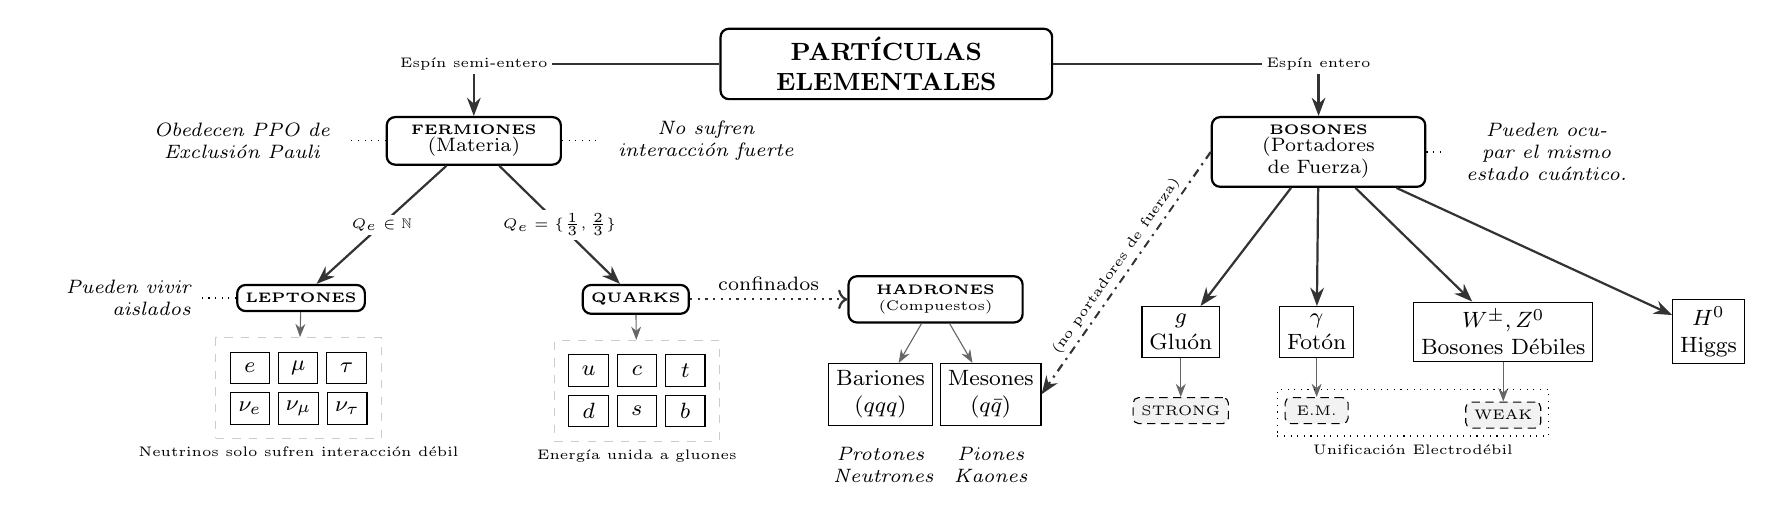
\begin{tikzpicture}[ 
% --- CONFIGURACIÓN DE ESTILOS --- 
node distance=1.5cm and 1.0cm, 
% Fuente base
% font=\rmfamily,
% Cajas principales 
box/.style={ draw=black, thick, fill=white, rounded corners=3pt, align=center, inner sep=3pt, font=\rmfamily\tiny\bfseries }, 
% Cajas de partículas específicas
particle/.style={ draw=black, thin, fill=white, minimum width=0.5cm, minimum height=0.4cm, align=center, font=\rmfamily\footnotesize }, 
% Notas y propiedades (texto lateral) 
note/.style={ draw=none, fill=none, align=left, font=\rmfamily\scriptsize\itshape, text width=2.5cm, inner sep=2pt }, 
% Estilo para las interacciones (fuerzas) 
force/.style={ draw=black, densely dashed, fill=white!95!black, rounded corners=2pt, align=center, font=\rmfamily\tiny, minimum width=0.8cm, inner sep=3pt },
% Conectores 
line/.style={-Stealth, thick, draw=black!80}, connector/.style={-Stealth, thin, draw=black!60}, labelline/.style={midway, fill=white, font=\rmfamily\tiny, inner sep=1.5pt} ]

% =============================================
% NIVEL 0: RAÍZ
% =============================================

\node[box, text width=4cm, font=\rmfamily\small\bfseries] (root) {PARTÍCULAS ELEMENTALES};

% =============================================
% NIVEL 1: CLASIFICACIÓN POR ESPÍN
% =============================================
\node[box, below left=0.2cm and 2.0cm of root, text width=2cm] (fermiones) {FERMIONES\\ \normalfont\scriptsize(Materia)};
\node[box, below right=0.2cm and 2.0cm of root, text width=2.5cm] (bosones) {BOSONES\\ \normalfont\scriptsize(Portadores de Fuerza)};

\draw[line] (root) -| node[labelline] {Espín semi-entero} (fermiones);
\draw[line] (root) -| node[labelline] {Espín entero} (bosones);

% --- Notas de Estadística ---
\node[note, left=0.5cm of fermiones, align=center] (stat_fermi) {Obedecen PPO de\\Exclusión Pauli};
\node[note, right=0.5cm of fermiones, align=center] (stat_fermi_2) {No sufren\\interacción fuerte};
\node[note, right=0.2cm of bosones, align=center] (stat_bose) {Pueden ocupar el mismo estado cuántico.};

\draw[dotted, thin] (fermiones) -- (stat_fermi);
\draw[dotted, thin] (fermiones) -- (stat_fermi_2);
\draw[dotted, thin] (bosones) -- (stat_bose);


% =============================================
% NIVEL 2: FAMILIAS DE FERMIONES
% =============================================
\node[box, below left=1.5cm and 0.25cm of fermiones] (leptones) {LEPTONES};
\node[box, below right=1.5cm and 0.25cm of fermiones] (quarks) {QUARKS};

\draw[line] (fermiones) -- node[labelline] {$Q_e \in \mathbb{N}$} (leptones);
\draw[line] (fermiones) -- node[labelline] {$Q_e =\{\frac{1}{3}, \tfrac{2}{3}\}$} (quarks);

% --- Notas Leptones/Quarks ---
\node[note, left=0.5cm of leptones, align=right, text width=2cm] (prop_lept) {Pueden vivir aislados};

\draw[dotted, thin] (leptones) -- (prop_lept);

% =============================================
% NIVEL 3: GENERACIONES (Matrices de Partículas)
% =============================================

% --- MATRIZ LEPTONES ---
% Generación 1, 2, 3
\node[particle, below=0.5cm of leptones, xshift=-0.65cm] 
(e) {$e$};
\node[particle, right=0.1 of e] (mu) {$\mu$};
\node[particle, right=0.1cm of mu] (tau) {$\tau$};

\node[particle, below=0.1cm of e] (nue) {$\nu_e$};
\node[particle, right=0.1cm of nue] (numu) {$\nu_\mu$};
\node[particle, right=0.1cm of numu] (nutau) {$\nu_\tau$};

\node[fit=(e)(nutau), draw=black!20, dashed, inner sep=5pt, label={[font=\tiny]below:Neutrinos solo sufren interacción débil}] (box_lept) {};
\draw[connector] (leptones) -- (box_lept);

% --- MATRIZ QUARKS ---
\node[particle, below=0.5cm of quarks, xshift=-0.60cm] (u) {$u$};
\node[particle, right=0.1cm of u] (c) {$c$};
\node[particle, right=0.1cm of c] (t) {$t$};

\node[particle, below=0.1cm of u] (d) {$d$};
\node[particle, right=0.1cm of d] (s) {$s$};
\node[particle, right=0.1cm of s] (b) {$b$};

\node[fit=(u)(b), draw=black!20, dashed, inner sep=5pt, label={[font=\tiny]below:Energía unida a gluones}] (box_quark) {};
\draw[connector] (quarks) -- (box_quark);

% =============================================
% NIVEL 2.5: HADRONES (Derivado de Quarks)
% =============================================
% 1. Definimos el nodo Hadrones a la derecha
\node[box, right=2cm of quarks, text width=2cm, scale=1] (hadrones) {HADRONES\\ \normalfont\tiny(Compuestos)};
\draw[line, dotted, ->] (quarks.east) -- (hadrones.west) 
    node[midway, above, font=\scriptsize] {confinados};

\node[particle, below=0.5cm of hadrones, xshift=-0.7cm, minimum width=1.2cm] (bariones) {Bariones\\($qqq$)};
\node[particle, below=0.5cm of hadrones, xshift=0.7cm, minimum width=1.2cm] (mesones) {Mesones\\($q\bar{q}$)};

\draw[connector] (hadrones) -- (bariones);
\draw[connector] (hadrones) -- (mesones);
\node[note, below=0.2cm of bariones, text width=1.2cm, align=center] {Protones\\Neutrones};
\node[note, below=0.2cm of mesones, text width=1.2cm, align=center] {Piones\\Kaones};

% =============================================
% NIVEL 3: BOSONES GAUGE (Fuerzas)
% =============================================

% Dividimos bosones en Gauge y Escalar
\node[particle, below=1.5cm of bosones, xshift=-1.75cm] (gluon) {$g$\\Gluón};
\node[particle, right=0.75cm of gluon] (photon) {$\gamma$\\Fotón};
\node[particle, right=0.75cm of photon] (wz) {$W^\pm, Z^0$\\Bosones Débiles};

% Bosón de Higgs aparte
\node[particle, right=1cm of wz] (higgs) {$H^0$\\Higgs};

\draw[line] (bosones) -- (gluon);
\draw[line] (bosones) -- (photon);
\draw[line] (bosones) -- (wz);
\draw[line] (bosones) -- (higgs);

% =============================================
% NIVEL 4: INTERACCIONES FUNDAMENTALES
% =============================================
\node[force, below=0.5cm of gluon] (f_fuerte) {STRONG};
\node[force, below=0.5cm of photon] (f_em) {E.M.};
\node[force, below=0.5cm of wz] (f_debil) {WEAK};

\draw[connector] (gluon) -- (f_fuerte);
\draw[connector] (photon) -- (f_em);
\draw[connector] (wz) -- (f_debil);

% Unificación Electrodébil
\node[draw, dotted, fit=(f_em)(f_debil), label={[font=\tiny]below:Unificación Electrodébil}] {};

% =============================================
% CONEXIONES CRUZADAS (Física Rigurosa)
% =============================================
\draw[line, dash dot] (bosones.west) to node[labelline, rotate=55, anchor=south] {(no portadores de fuerza)} (mesones.east);

\end{tikzpicture}
\end{adjustbox}



\section{PROPIEDADES DE MESONES (ESTADOS LIGADOS)}

{
\centering
\begin{tabular}{|l|c|c|c|c|l|l|l|}
\hline
\textbf{Mesón} & $I$ & $S$ & $J^\pi$ & $I_3$ & \textbf{m (MeV)} & $\tau$ \textbf{(s)} & \textbf{Decays} \\ \hline
$\pi^+$ & 1 & 0 & $0^-$ & +1 & 139.57039 & $2.6033 \cdot 10^{-8}$ & $\mu^+\nu_\mu$ \\ \hline
$\pi^0$ & 1 & 0 & $0^-$ & 0 & 134.9768 & $8.43 \cdot 10^{-17}$ & $2\gamma$ \\ \hline
$\pi^-$ & 1 & 0 & $0^-$ & -1 & 139.57039 & $2.6033 \cdot 10^{-8}$ & $\mu^-\bar{\nu}_\mu$ \\ \hline
$\eta$ & 0 & 0 & $0^-$ & 0 & 547.862 & $\Gamma = 1.31$ keV & $2\gamma$ \\ \hline
$K^+$ & 1/2 & 1 & $0^-$ & 1/2 & 493.677 & $1.2380 \cdot 10^{-8}$ & $\pi^+\pi^0, \mu^+\nu_\mu$ \\ \hline
$K^0$ & 1/2 & 1 & $0^-$ & -1/2 & 497.611 & $0.8954 \cdot 10^{-10} $ & $2\pi, 3\pi$ \\ \hline
$\bar{K}^0$ & 1/2 & -1 & $0^-$ & 1/2 & 497.611 & $5.116 \cdot 10^{-8}$ & $2\pi, 3\pi$ \\ \hline
$K^-$ & 1/2 & -1 & $0^-$ & -1/2 & 493.677& $1.2380\cdot 10^{-8}$ & $\pi^-\pi^0, \mu^-\bar{\nu}_\mu$ \\ \hline
\end{tabular}

}

\section{RESONANCIAS MESÓNICAS}

{
\centering
\begin{tabular}{|l|c|c|c|c|l|l|l|}
\hline
\textbf{Mesón} & $I$ & $S$ & $J^\pi$ & $I_3$ & \textbf{Masa (MeV)} & $\Gamma$ \textbf{(MeV)} & \textbf{Deca.} \\ \hline
$\rho^+(770)$ & 1 & 0 & $1^-$ & 1 & 775.26(23) & 149.1(8) & $2\pi$ \\ \hline
$\rho^0(770)$ & 1 & 0 & $1^-$ & 0 & 775.26(23) & 149.1(8) & $2\pi$ \\ \hline
$\rho^-(770)$ & 1 & 0 & $1^-$ & -1 & 775.26(23) & 149.1(8) & $2\pi$ \\ \hline
$\omega(783)$ & 0 & 0 & $1^-$ & 0 & 782.66(13)5 & 8.68(13) & $3\pi$ \\ \hline
$\eta'(958)$ & 0 & 0 & $0^-$ & 0 & 957.78(6) & 0.188(6) & $\eta 2\pi$ \\ \hline
$\phi(1020)$ & 0 & 0 & $1^-$ & 0 & 1019.461(16) & 4.249(13) & $K\bar{K}$ \\ \hline
$K^+(892)$ & 1/2 & 1 & $1^-$ & 1/2 & 891.67(26) & 51.4(8) & $K\pi$ \\ \hline
$K^0(892)$ & 1/2 & 1 & $1^-$ & -1/2 & 895.55(20) & 47.3(5) & $K\pi$ \\ \hline
$\bar{K}^0(892)$ & 1/2 & -1 & $1^-$ & 1/2 & 895.55(20) & 47.3(5) & $K\pi$ \\ \hline
$K^-(892)$ & 1/2 & -1 & $1^-$ & -1/2 & 891.67(26) & 51.4(8) & $K\pi$ \\ \hline
\end{tabular}

}


\section{PROPIEDADES DE BARIONES (ESTADOS FUNDAMENTALES)}

{
\centering
\begin{tabular}{|l|c|c|c|c|l|l|l|}
\hline
\textbf{Barión} & $I$ & $S$ & $J^\pi$ & $I_3$ & \textbf{m (MeV)} & $\tau$ \textbf{(s)} & \textbf{Decays} \\ \hline
p & 1/2 & 0 & $1/2^+$ & 1/2 & 938.27208816 & $> 9 \cdot 10^{29}$ y & - \\ \hline
n & 1/2 & 0 & $1/2^+$ & -1/2 & 939.5654205 & 878.4 & $p e \bar{\nu}_e$ \\ \hline
$\Lambda$ & 0 & -1 & $1/2^+$ & 0 & 1115.683 & $2.632 \cdot 10^{-10}$ & $N\pi$ \\ \hline
$\Sigma^+$ & 1 & -1 & $1/2^+$ & 1 & 1189.37 & $0.8018 \cdot 10^{-10}$ & $N\pi$ \\ \hline
$\Sigma^0$ & 1 & -1 & $1/2^+$ & 0 & 1192.642 & $7.4 \cdot 10^{-20}$ & $\Lambda\gamma$ \\ \hline
$\Sigma^-$ & 1 & -1 & $1/2^+$ & -1 & 1197.449 & $1.479 \cdot 10^{-10}$ & $N\pi$ \\ \hline
$\Xi^0$ & 1/2 & -2 & $1/2^+$ & 1/2 & 1314.86(20) & $2.90 \cdot 10^{-10}$ & $\Lambda\pi$ \\ \hline
$\Xi^-$ & 1/2 & -2 & $1/2^+$ & -1/2 & 1321.71 & $1.639 \cdot 10^{-10}$ & $\Lambda\pi$ \\ \hline
$\Omega^-$ & 0 & -3 & $3/2^+$ & 0 & 1672.45 & $0.821 \cdot 10^{-10}$ & $\Lambda K$ \\ \hline
\end{tabular}

}

\section{RESONANCIAS BARIÓNICAS}

{
\centering
\begin{tabular}{|l|c|c|c|c|l|l|l|}
\hline
\textbf{Barión} & $I$ & $S$ & $J^\pi$ & $I_3$ & \textbf{m (MeV)} & $\Gamma$ \textbf{(MeV)} & \textbf{Decays} \\ \hline
$\Delta^{++}(1232)$ & 3/2 & 0 & $3/2^+$ & +3/2 & 1232 & 117 & $N\pi$ \\ \hline
$\Delta^+(1232)$ & 3/2 & 0 & $3/2^+$ & +1/2 & 1232 & 117 & $N\pi$ \\ \hline
$\Delta^0(1232)$ & 3/2 & 0 & $3/2^+$ & -1/2 & 1232 & 117 & $N\pi$ \\ \hline
$\Delta^-(1232)$ & 3/2 & 0 & $3/2^+$ & -3/2 & 1232 & 117 & $N\pi$ \\ \hline
$N^+(1440)$ & 1/2 & 0 & $1/2^+$ & +1/2 & 1440 & 350 & $N\pi$ \\ \hline
$N^0(1440)$ & 1/2 & 0 & $1/2^+$ & -1/2 & 1440 & 350 & $N\pi$ \\ \hline
$\Lambda(1405)$ & 0 & -1 & $1/2^-$ & 0 & 1405.1 & 50.5 & $\Sigma\pi$ \\ \hline
$\Sigma^+(1385)$ & 1 & -1 & $3/2^+$ & 1 & 1382.83 & 36.2 & $\Lambda\pi$ \\ \hline
$\Sigma^0(1385)$ & 1 & -1 & $3/2^+$ & 0 & 1383.7 & 36 & $\Lambda\pi$ \\ \hline
$\Sigma^-(1385)$ & 1 & -1 & $3/2^+$ & -1 & 1387.2 & 39.4 & $\Lambda\pi$ \\ \hline
$\Xi^0(1530)$ & 1/2 & -2 & $3/2^+$ & 1/2 & 1531.80 & 9.1 & $\Xi\pi$ \\ \hline
$\Xi^-(1530)$ & 1/2 & -2 & $3/2^+$ & -1/2 & 1535.0 & 9.9 & $\Xi\pi$ \\ \hline
\end{tabular}

}


\section{HADRONES PESADOS: ESPECTROSCOPIA DE QUARKS $c$ Y $b$}
\vspace{0.1cm}

\begin{minipage}{0.48\linewidth}
    \centering
    \textbf{ENCANTO ($c$)}
    \begin{tabular}{|l|l|c|}
        \hline
        \textbf{Hadrón} & \textbf{Masa} & \textbf{Comp.} \\ \hline
        $J/\Psi$ & $3096.900$ & $c\bar{c}$ \\ \hline
        $D^+$ & $1869.66$ & $c\bar{d}$ \\ \hline
        $D^-$ & $1869.66$ & $d\bar{c}$ \\ \hline
        $D^0$ & $1864.84$ & $c\bar{u}$ \\ \hline
        $\bar{D}^0$ & $1864.84$ & $u\bar{c}$ \\ \hline
        $\Lambda_c^+$ & $2286.46$ & $cdu$ \\ \hline
    \end{tabular}
\end{minipage}
\hfill
\begin{minipage}{0.48\linewidth}
    \centering
    \textbf{BELLEZA ($b$)}
    \begin{tabular}{|l|l|c|}
        \hline
        \textbf{Hadrón} & \textbf{Masa} & \textbf{Comp.} \\ \hline
        $\Upsilon$ & $9460.40$ & $b\bar{b}$ \\ \hline
        $B^+$ & $5279.34$ & $u\bar{b}$ \\ \hline
        $B^-$ & $5279.34$ & $b\bar{u}$ \\ \hline
        $B^0$ & $5279.66$ & $d\bar{b}$ \\ \hline
        $\bar{B}^0$ & $5279.66$ & $b\bar{d}$ \\ \hline
        $\Lambda_b^0$ & $5619.69$ & $bdu$ \\ \hline
    \end{tabular}
\end{minipage}

\vspace{0.2cm}






\section{ESTRUCTURA DE VALENCIA DE HADRONES (QUARKS)}

{
\centering
\begin{tabular}{|l|l|l|l||l|l|l|l|}
\hline
\textbf{Mesón} & \textbf{qq} & \textbf{Mesón} & \textbf{qq} & \textbf{Barión} & \textbf{qqq} & \textbf{Barión} & \textbf{qqq} \\ \hline
$\pi^+$ & $u\bar{d}$ & $K^+$ & $u\bar{s}$ & $p$ & $uud$ & $\Sigma^-$ & $dds$ \\ \hline
$\pi^0$ & $u\bar{u}, d\bar{d}$ & $K^0$ & $d\bar{s}$ & $n$ & $udd$ & $\Lambda$ & $uds$ \\ \hline
$\pi^-$ & $d\bar{u}$ & $\bar{K}^0$ & $s\bar{d}$ & $\Sigma^+$ & $uus$ & $\Xi^0$ & $uss$ \\ \hline
$\eta$ & $u\bar{u}, d\bar{d}, s\bar{s}$ & $K^-$ & $s\bar{u}$ & $\Sigma^0$ & $uds$ & $\Xi^-$ & $dss$ \\ \hline
\hline
\textbf{Reson.} & \textbf{qq} & \textbf{Reson.} & \textbf{qq} & \textbf{Reson.} & \textbf{qqq} & \textbf{Reson.} & \textbf{qqq} \\ \hline
$\rho^+$ & $u\bar{d}$ & $\phi$ & $s\bar{s}$ & $\Delta^{++}$ & $uuu$ & $\Delta^-$ & $ddd$ \\ \hline
$\rho^0$ & $u\bar{u}, d\bar{d}$ & $K^{*+}$ & $u\bar{s}$ & $\Delta^+$ & $uud$ & $\Omega^-$ & $sss$ \\ \hline
$\omega$ & $u\bar{u}, d\bar{d}$ & & & $\Delta^0$ & $udd$ & & \\ \hline
\end{tabular}

}


\section{TABLA DE CONFIGURACIONES DE COLOR}
{
\centering
\begin{center}
\begin{tabular}{|l|c|c|}
\hline
\textbf{Sistema} & \textbf{Estado de color} & \textbf{Interacción} \\ \hline
$q - q$ & $(|rv\rangle - |vr\rangle)/\sqrt{2}$ & \textbf{Atractiva} \\ \hline
$q - q$ & $(|rv\rangle + |vr\rangle)/\sqrt{2}$ & \textbf{Repulsiva} \\ \hline
$q - \bar{q}$ & $(|r\bar{r}\rangle + |v\bar{v}\rangle + |a\bar{a}\rangle)/\sqrt{3}$ & \textbf{Atractiva} \\ \hline
$q - \bar{q}$ & $|r\bar{v}\rangle$ & \textbf{Repulsiva} \\ \hline
$q - q - q$ & $A_{123}|rva\rangle$ & \textbf{Atractiva} \\ \hline
$q - q - q$ & $(|rva\rangle + |rav\rangle)/\sqrt{2}$ & \textbf{Repulsiva} \\ \hline
\end{tabular}
\end{center}

}


% Estilos TikZ para partículas y líneas
\tikzset{
    particle/.style={circle, fill=black, inner sep=1.5pt, outer sep=2pt},
    label_node/.style={font=\bfseries\small},
    charge_line/.style={blue!60, thick},      % Líneas diagonales (Carga Q)
    strange_line/.style={red!60, thick, dashed}, % Líneas horizontales (Extrañeza S)
    axis_label/.style={font=\tiny\itshape}
}


\hypertarget{Mesones}{\section*{Octete de Mesones ($J^P=0^-$)}}


{
\centering
% --- DIAGRAMA 1: OCTETE DE MESONES (J^P = 0^-) ---
\begin{tikzpicture}[scale=0.75]
    % Coordenadas (Eje X = I3 * 2, Eje Y = S * 1.5)
    \coordinate (K0) at (-1, 1.5);   % S=1, I3=-1/2
    \coordinate (Kp) at (1, 1.5);    % S=1, I3=1/2
    \coordinate (pim) at (-2, 0);    % S=0, I3=-1
    \coordinate (pi0) at (0, 0);     % S=0, I3=0
    \coordinate (pip) at (2, 0);     % S=0, I3=1
    \coordinate (Km) at (-1, -1.5);  % S=-1, I3=-1/2
    \coordinate (K0b) at (1, -1.5);  % S=-1, I3=1/2

    % Líneas de Estructura (Hexágono)
    \draw[thick] (K0) -- (Kp) -- (pip) -- (K0b) -- (Km) -- (pim) -- cycle;

    % Líneas de Carga Q (Azul)
    \draw[charge_line] ($(pim)+(-0.5,0.75)$) -- ($(Km)+(0.5,-0.75)$) node[below] {\tiny $Q=-1$};
    \draw[charge_line] ($(K0)+(-0.5,0.75)$) -- ($(K0b)+(0.5,-0.75)$) node[below] {\tiny $Q=0$};
    \draw[charge_line] ($(Kp)+(-0.5,0.75)$) -- ($(pip)+(0.5,-0.75)$) node[below] {\tiny $Q=+1$};

    % Líneas de Extrañeza S (Rojo)
    \draw[strange_line] (-2.2, 1.5) node[left] {\color{red} $S=+1$} -- (2.2, 1.5);
    \draw[strange_line] (-2.75, 0) node[left] {\color{red} $S=0$} -- (2.5, 0);
    \draw[strange_line] (-2.2, -1.5) node[left] {\color{red} $S=-1$} -- (2.2, -1.5);

    % Partículas
    \node[particle] at (K0) {}; \node[above right] at (K0) {$K^0$};
    \node[particle] at (Kp) {}; \node[above right] at (Kp) {$K^+$};
    \node[particle] at (pim) {}; \node[above left] at (pim) {$\pi^-$};
    \node[particle] at (pi0) {}; \node[above right] at (pi0) {$\pi^0$};
    \node[particle] at (0, -0.3) {}; \node[below left] at (0, -0.3) {$\eta^0$};
    \node[particle] at (pip) {}; \node[above right] at (pip) {$\pi^+$};
    \node[particle] at (Km) {}; \node[below left] at (Km) {$K^-$};
    \node[particle] at (K0b) {}; \node[below left] at (K0b) {$\overline{K}^0$};

\end{tikzpicture}

}

{\section*{Octete de Mesones ($J^P=1^-$)}}

{
\centering
% --- DIAGRAMA 1: OCTETE DE MESONES (J^P = 1^-) ---
\begin{tikzpicture}[scale=0.75]
    % Coordenadas (Eje X = I3 * 2, Eje Y = S * 1.5)
    \coordinate (K0) at (-1, 1.5);   % S=1, I3=-1/2
    \coordinate (Kp) at (1, 1.5);    % S=1, I3=1/2
    \coordinate (pim) at (-2, 0);    % S=0, I3=-1
    \coordinate (pi0) at (0, 0);     % S=0, I3=0
    \coordinate (pip) at (2, 0);     % S=0, I3=1
    \coordinate (Km) at (-1, -1.5);  % S=-1, I3=-1/2
    \coordinate (K0b) at (1, -1.5);  % S=-1, I3=1/2

    % Líneas de Estructura (Hexágono)
    \draw[thick] (K0) -- (Kp) -- (pip) -- (K0b) -- (Km) -- (pim) -- cycle;

    % Líneas de Carga Q (Azul)
    \draw[charge_line] ($(pim)+(-0.5,0.75)$) -- ($(Km)+(0.5,-0.75)$) node[below] {\tiny $Q=-1$};
    \draw[charge_line] ($(K0)+(-0.5,0.75)$) -- ($(K0b)+(0.5,-0.75)$) node[below] {\tiny $Q=0$};
    \draw[charge_line] ($(Kp)+(-0.5,0.75)$) -- ($(pip)+(0.5,-0.75)$) node[below] {\tiny $Q=+1$};

    % Líneas de Extrañeza S (Rojo)
    \draw[strange_line] (-2.2, 1.5) node[left] {\color{red} $S=+1$} -- (2.2, 1.5);
    \draw[strange_line] (-2.75, 0) node[left] {\color{red} $S=0$} -- (2.5, 0);
    \draw[strange_line] (-2.2, -1.5) node[left] {\color{red} $S=-1$} -- (2.2, -1.5);

    % Partículas
    \node[particle] at (K0) {}; \node[above right] at (K0) {$K^{*0}$};
    \node[particle] at (Kp) {}; \node[above right] at (Kp) {$K^{*+}$};
    \node[particle] at (pim) {}; \node[above left] at (pim) {$\rho^-$};
    \node[particle] at (pi0) {}; \node[above right] at (pi0) {$\rho^0$};
    \node[particle] at (0, -0.3) {}; \node[below left] at (0, -0.3) {$\omega^0$};
    \node[particle] at (pip) {}; \node[above right] at (pip) {$\rho^+$};
    \node[particle] at (Km) {}; \node[below left] at (Km) {$K^{*-}$};
    \node[particle] at (K0b) {}; \node[below left] at (K0b) {$\overline{K}^{*0}$};

\end{tikzpicture}

}

% --- DIAGRAMA 2: OCTETE DE BARIONES (J^P = 1/2^+) ---
\hypertarget{Bariones}{\section*{Octete de Bariones ($J^P=1/2^+$)}}

{
\centering
\begin{tikzpicture}[scale=0.75]
    % Coordenadas
    \coordinate (n) at (-1, 1.5);    % S=0, I3=-1/2
    \coordinate (p) at (1, 1.5);     % S=0, I3=1/2
    \coordinate (Sm) at (-2, 0);     % S=-1, I3=-1
    \coordinate (S0) at (0, 0);      % S=-1, I3=0
    \coordinate (Sp) at (2, 0);      % S=-1, I3=1
    \coordinate (Xm) at (-1, -1.5);  % S=-2, I3=-1/2
    \coordinate (X0) at (1, -1.5);   % S=-2, I3=1/2

    % Hexágono
    \draw[thick] (n) -- (p) -- (Sp) -- (X0) -- (Xm) -- (Sm) -- cycle;

    % Líneas Q
    \draw[charge_line] ($(Sm)+(-0.5,0.75)$) -- ($(Xm)+(0.5,-0.75)$) node[below] {\tiny $Q=-1$};
    \draw[charge_line] ($(n)+(-0.5,0.75)$) -- ($(X0)+(0.5,-0.75)$) node[below] {\tiny $Q=0$};
    \draw[charge_line] ($(p)+(-0.5,0.75)$) -- ($(Sp)+(0.5,-0.75)$) node[below] {\tiny $Q=+1$};

    % Líneas S
    \draw[strange_line] (-2.2, 1.5) node[left] {\color{red} $S=0$} -- (2.2, 1.5);
    \draw[strange_line] (-2.75, 0) node[left] {\color{red} $S=-1$} -- (2.5, 0);
    \draw[strange_line] (-2.2, -1.5) node[left] {\color{red} $S=-2$} -- (2.2, -1.5);

    % Partículas
    \node[particle] at (n) {}; \node[above right] at (n) {$n$};
    \node[particle] at (p) {}; \node[above right] at (p) {$p$};
    \node[particle] at (Sm) {}; \node[above left] at (Sm) {$\Sigma^-$};
    \node[particle] at (S0) {}; \node[above right] at (S0) {$\Sigma^0$};
    \node[particle] at (0, -0.3) {}; \node[below left] at (0, -0.3) {$\Lambda$};
    \node[particle] at (Sp) {}; \node[above right] at (Sp) {$\Sigma^+$};
    \node[particle] at (Xm) {}; \node[below left] at (Xm) {$\Xi^-$};
    \node[particle] at (X0) {}; \node[below left] at (X0) {$\Xi^0$};

\end{tikzpicture}

}

% --- DIAGRAMA 3: DECUPLETE DE BARIONES (J^P = 3/2^+) ---
\hypertarget{Bariones_big}{\section*{Decuplete de Bariones ($J^P=3/2^+$)}}

{
\centering
\begin{tikzpicture}[scale=0.6]
    % Coordenadas (Triángulo Invertido)
    % Fila S=0 (Deltas)
    \coordinate (Dmm) at (-3, 2.25); % I3=-3/2
    \coordinate (Dm) at (-1, 2.25);  % I3=-1/2
    \coordinate (D0) at (1, 2.25);   % I3=1/2
    \coordinate (Dp) at (3, 2.25);   % I3=3/2
    
    % Fila S=-1 (Sigmas*)
    \coordinate (Sms) at (-2, 0.75); % I3=-1
    \coordinate (S0s) at (0, 0.75);  % I3=0
    \coordinate (Sps) at (2, 0.75);  % I3=1
    
    % Fila S=-2 (Xi*)
    \coordinate (Xms) at (-1, -0.75);% I3=-1/2
    \coordinate (X0s) at (1, -0.75); % I3=1/2
    
    % Fila S=-3 (Omega)
    \coordinate (Om) at (0, -2.25);  % I3=0

    % Estructura
    \draw[thick] (Dmm) -- (Dp) -- (Om) -- cycle;

    % Definición del vector director base
    \coordinate (Start_Q_minus1) at ($(Dmm)+(-0.60,0.95)$);
    \path let \p1 = ($(Om)-(Start_Q_minus1)$) in coordinate (vec) at (\x1,\y1);
    
    % --- Q = -1 ---
    % Escalar 1.1 ANTES del vector
    \draw[charge_line] (Start_Q_minus1) -- ++($ 1.1*(vec) $) 
        node[right] {\tiny $Q=-1$};
    
    % --- Q = 0 ---
    \draw[charge_line] ($(Dm)+(-0.5,0.75)$) -- ++($ 0.8*(vec) $) 
        node[right, xshift=5pt] {\tiny $Q=0$};
    
    % --- Q = 1 ---
    \draw[charge_line] (0.55,3) -- ++($ 0.50*(vec) $) 
        node[right, xshift=5pt] {\tiny $Q=1$};
    
    % --- Q = 2 ---
    \draw[charge_line] (2.5,3) -- ++($ 0.3*(vec) $) 
        node[right, xshift=5pt] {\tiny $Q=2$};
    
    % Líneas S
    \draw[strange_line] (-3.5, 2.25) node[left] {\color{red} $S=0$} -- (3.5, 2.25);
    \draw[strange_line] (-2.95, 0.75) node[left] {\color{red} $S=-1$} -- (2.5, 0.75);
    \draw[strange_line] (-1.95, -0.75) node[left] {\color{red} $S=-2$} -- (1.5, -0.75);
    \draw[strange_line] (-0.5, -2.25) node[left] {\color{red} $S=-3$} -- (0.5, -2.25);

    % Partículas
    \node[particle] at (Dmm) {}; \node[above right] at (Dmm) {$\Delta^-$};
    \node[particle] at (Dm) {}; \node[above right] at (Dm) {$\Delta^0$};
    \node[particle] at (D0) {}; \node[above right] at (D0) {$\Delta^+$};
    \node[particle] at (Dp) {}; \node[above right] at (Dp) {$\Delta^{++}$};
    
    \node[particle] at (Sms) {}; \node[above left] at (Sms) {$\Sigma^{*-}$};
    \node[particle] at (S0s) {}; \node[above right] at (S0s) {$\Sigma^{*0}$};
    \node[particle] at (Sps) {}; \node[above right] at (Sps) {$\Sigma^{*+}$};
    
    \node[particle] at (Xms) {}; \node[above left] at (Xms) {$\Xi^{*-}$};
    \node[particle] at (X0s) {}; \node[above right] at (X0s) {$\Xi^{*0}$};
    
    \node[particle] at (Om) {}; \node[below left] at (Om) {$\Omega^-$};

\end{tikzpicture}

}

\hypertarget{Gluones}{\section*{Octuplete de Gluones}}


{
\centering
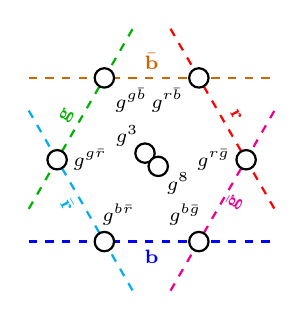
\begin{tikzpicture}[scale=1.2, >=latex]
    % Definición de coordenadas
    \coordinate (Center) at (0,0);
    \coordinate (Gr) at (-1, 0);       % g^{g \bar{r}}
    \coordinate (Rg) at (1, 0);        % g^{r \bar{g}}
    \coordinate (Gb) at (-0.5, 0.866); % g^{g \bar{b}}
    \coordinate (Rb) at (0.5, 0.866);  % g^{r \bar{b}}
    \coordinate (Br) at (-0.5, -0.866);% g^{b \bar{r}}
    \coordinate (Bg) at (0.5, -0.866); % g^{b \bar{g}}

    % --- LÍNEAS DE FLUJO DE COLOR (Ejes Discontinuos) ---
    % Los colores se han ajustado para coincidir con la imagen proporcionada

    % 1. Ejes Horizontales
    % Anti-blue (Naranja)
    \draw[dashed, color=orange!80!black, thick] (-1.3, 0.866) -- (1.3, 0.866) 
        node[midway, above, font=\bfseries] {$\bar{\textbf{b}}$};
    % Blue (Azul)
    \draw[dashed, color=blue, thick] (-1.3, -0.866) -- (1.3, -0.866) 
        node[midway, below, font=\bfseries] {b};

    % 2. Ejes Diagonales \ (Verde / Magenta)
    % Green (Verde)
    \draw[dashed, color=green!70!black, thick] (-1.3, -0.52) -- (-0.2, 1.386) 
        node[pos=0.75, left, rotate=60, font=\bfseries, xshift = -15pt, yshift=5pt] {g};
    % Anti-green (Magenta)
    \draw[dashed, color=magenta, thick] (0.2, -1.386) -- (1.3, 0.52) 
        node[pos=0.25, right, rotate=60, font=\bfseries, xshift=15pt, yshift=-4pt] {$\bar{\textbf{g}}$};

    % 3. Ejes Diagonales / (Cian / Rojo)
    % Anti-red (Cian)
    \draw[dashed, color=cyan, thick] (-1.3, 0.52) -- (-0.2, -1.386) 
        node[pos=0.75, left, rotate=-60, font=\bfseries, xshift=-15pt,yshift=-5pt] {$\bar{\textbf{r}}$};
    % Red (Rojo)
    \draw[dashed, color=red, thick] (0.2, 1.386) -- (1.3, -0.52) 
        node[pos=0.25, right, rotate=-60, font=\bfseries, xshift=15, yshift=5pt] {r};

    % --- NODOS (Partículas) ---
    % Círculos más grandes con borde grueso
    \tikzset{gluon/.style={fill=white, draw=black, thick, circle, minimum size=7pt, inner sep=0pt}}

    \node[gluon] at (Gr) {};
    \node[gluon] at (Rg) {};
    \node[gluon] at (Gb) {};
    \node[gluon] at (Rb) {};
    \node[gluon] at (Br) {};
    \node[gluon] at (Bg) {};

    % Nodo central doble
    \node[gluon] at (-0.07, 0.07) {};
    \node[gluon] at (0.07, -0.07) {};

    % --- ETIQUETAS (Estados de los gluones) ---
    % Posiciones ajustadas para coincidir con la imagen
    \node[right, xshift=1pt, yshift = -8pt] at (Gb) {$g^{g\bar{b}}$};
    \node[left, xshift=-3pt, yshift = -8pt] at (Rb) {$g^{r\bar{b}}$};
    \node[right, xshift=3pt] at (Gr) {$g^{g\bar{r}}$};
    \node[left, xshift=-3pt] at (Rg) {$g^{r\bar{g}}$};
    \node[above, xshift = 5pt, yshift=3pt] at (Br) {$g^{b\bar{r}}$};
    \node[above, xshift=-5pt, yshift=3pt] at (Bg) {$g^{b\bar{g}}$};

    % Etiquetas centrales
    \node[left, xshift=-2pt] at (0, 0.25) {$g^3$};
    \node[right, xshift=2pt] at (0.02, -0.25) {$g^8$};

\end{tikzpicture}


}




\clearpage
    
\end{multicols}

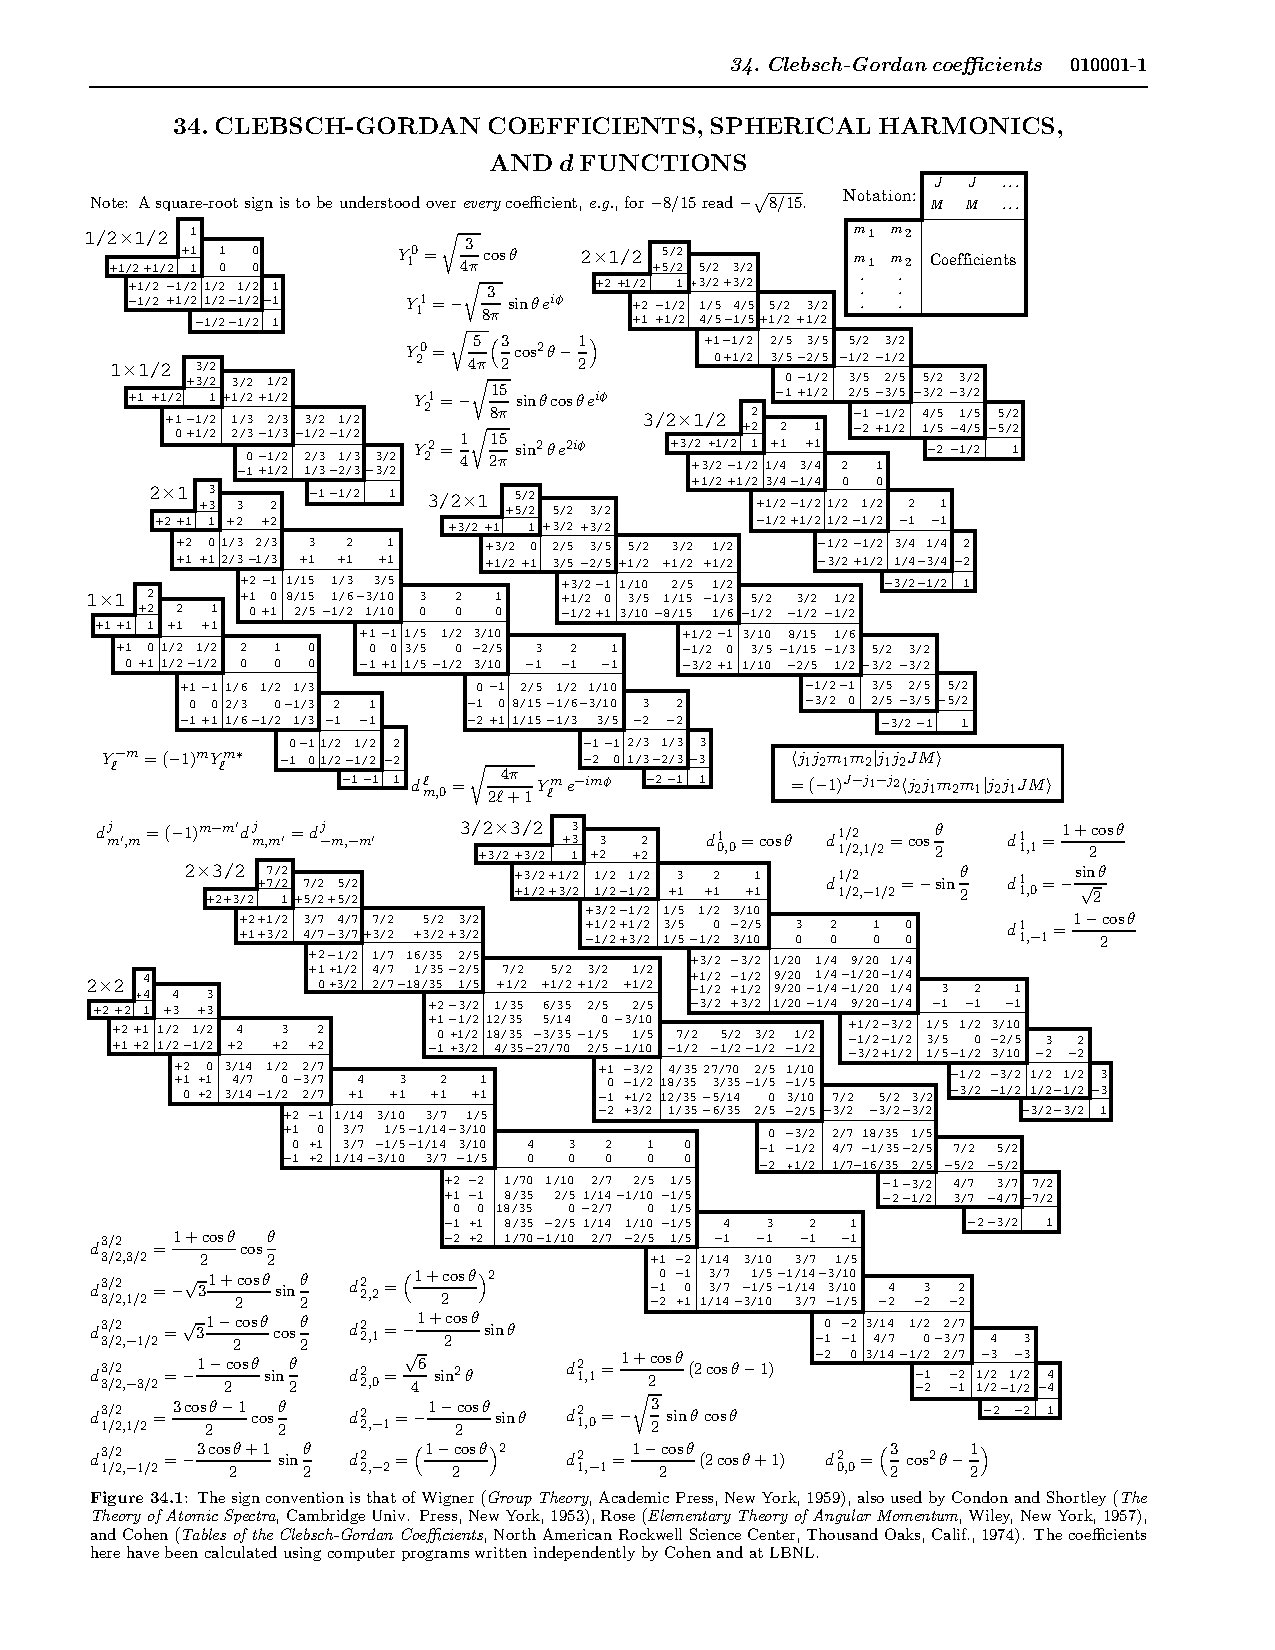
\includepdf[pages=1, angle=90]{pdfs/clebrpp.pdf}   

\end{document}